\documentclass[12pt]{report}
% English hyphenation
\usepackage[british]{babel}
% Links
\usepackage[breaklinks=true]{hyperref}
% Images
\usepackage{graphicx}
\graphicspath{ {./images/} }

\usepackage[noabbrev]{cleveref}

\crefname{appsec}{Appendix}{Appendices}

\usepackage[utf8]{inputenc}
\usepackage{csquotes}
\usepackage{booktabs} % 加在导言区，只需要引入一次
\usepackage{booktabs}
\usepackage{array}
\usepackage{colortbl}
\usepackage{esdiff}
\usepackage{multirow}
\usepackage{booktabs}
\usepackage{caption}
\usepackage{subcaption}
\usepackage[a4paper, headheight=15pt]{geometry}
\usepackage{algorithm}
\usepackage[load-configurations=abbreviations, binary-units=true]{siunitx}
\usepackage{algpseudocode}

\usepackage{fancyhdr}
\pagestyle{fancy}
\fancyhead{}
\fancyhead[L]{\leftmark}
\fancyhead[R]{\rightmark}
\fancyfoot{}
\fancyfoot[C]{\thepage}
\renewcommand{\headrulewidth}{0.4pt}
\renewcommand{\footrulewidth}{0.4pt}
\renewcommand{\chaptermark}[1]{ \markboth{#1}{} }
\renewcommand{\sectionmark}[1]{ \markright{#1}{} }

% Source images
\newcommand{\imagesource}[1] {\caption*{\begin{footnotesize} Source: \url{#1} \end{footnotesize}}}

% Appendix
\usepackage[toc,page]{appendix}
% Change name of toc
\renewcommand*\contentsname{Table of Contents}

\usepackage[style=numeric,sorting=none]{biblatex}
\addbibresource{bibliography.bib}

\title{}
\author{}
\date{April 2023}


\begin{document}

\begin{titlepage}
	\newcommand{\HRule}{\rule{\linewidth}{0.5mm}} % Defines a new command for horizontal lines, change thickness here
	
	\center % Centre everything on the page
	
	%------------------------------------------------
	%	Headings
	%------------------------------------------------
	
	\textsc{\LARGE University of Manchester}\\[0.75cm] % Main heading such as the name of your university/college
	
	\textsc{\Large School of Computer Science}\\[0.75cm] % Major heading such as course name
	
    
	% \textsc{\large BSc Artificial Intelligence\\
	% with Industrial Experience}\\[1.25cm] % Minor heading such as course title
	
	%------------------------------------------------
	%	Title
	%------------------------------------------------
	
	\HRule\\[0.4cm]
	
	{\huge\bfseries Perturbation is All You Need\\}\\[0.4cm] % Title of your document
	
	\HRule\\[1.5cm]
	
	%------------------------------------------------
	%	Author(s)
	%------------------------------------------------
	
	\begin{minipage}{0.4\textwidth}
		\begin{flushleft}
                \centering
			\large
			\textit{Author}\\
			Yongjiang \textsc{Liu} % Your name
		\end{flushleft}
	\end{minipage}
	~
	\begin{minipage}{0.4\textwidth}
		\begin{flushright}
			\large
			\textit{Supervisor}\\
			Dr. Francisco  \textsc{Lobo} % Supervisor's name
		\end{flushright}
	\end{minipage}
	
	\vfill
	
	
\includegraphics[width=0.3\textwidth]{crest.jpg}

    \vfill
    
	{\large April 2025} % Date, change the \today to a set date if you want to be precise

\end{titlepage}
\newpage
\section*{Abstract}
This study addresses the Electric Vehicle Routing Problem (EVRP), an important extension of the classical Vehicle Routing Problem that incorporates energy and load constraints. To tackle the challenges of ensuring route feasibility under limited battery capacities while achieving high-quality solutions, three advanced metaheuristic frameworks are developed: a Genetic Algorithm (GA), a Simulated Annealing (SA) approach, and an optimized Ant Colony Optimization (ACO) method. Each framework systematically integrates perturbation-driven diversification, adaptive local search mechanisms, and problem-specific repair strategies to enhance solution quality and robustness.

Comprehensive experiments were conducted on standard EVRP benchmark sets, covering both small- and large-scale instances. The proposed algorithms were evaluated against a Greedy Search baseline under unified experimental settings, measuring total travel distance, solution feasibility, computational efficiency, and robustness over multiple independent runs.

Results demonstrate that all three metaheuristics significantly outperform the baseline, with GA consistently achieving the best performance in terms of solution quality and stability. Systematic parameter sensitivity analyses further validate the critical roles of perturbation strategies, adaptive control mechanisms, and multi-stage local search in improving search effectiveness.

Overall, this work highlights the effectiveness and scalability of perturbation-driven metaheuristic optimization for solving complex, energy-constrained routing problems and points toward promising future directions for dynamic and multi-objective EVRP scenarios.


\newpage
\section*{Acknowledgements}

First and foremost, I would like to express my heartfelt gratitude to my supervisor, Dr. Francisco Lobo. His unwavering guidance, encouragement, and profound knowledge have been a source of inspiration throughout this journey. His patience, insightful advice, and continuous support have not only shaped this project but have also deeply influenced my growth as a scholar.

I am equally indebted to my beloved family. Their unconditional love, steadfast support, and unshakeable belief in me have been the foundation upon which I have built this achievement. Through every challenge and every moment of doubt, they stood by me, offering strength, hope, and endless encouragement. This accomplishment is as much theirs as it is mine.

To all those who have walked this path with me — thank you from the depths of my heart.

\newpage
\section*{List of Abbreviations}

\begin{tabular}{ll}
ACO & Ant Colony Optimization \\
EV & Electric Vehicle \\
EVRP & Electric Vehicle Routing Problem \\
GA & Genetic Algorithm \\
GHG & Greenhouse Gas \\
ICE & Internal Combustion Engine \\
MIP & Mixed Integer Programming \\
SA & Simulated Annealing \\
VRP & Vehicle Routing Problem \\
VRPTW & Vehicle Routing Problem with Time Windows \\
\end{tabular}


\pagenumbering{roman}

\tableofcontents

\listoffigures

\listoftables



\chapter{Introduction}
\pagenumbering{arabic}
\setcounter{page}{1}
\newpage
\section{Broad Overview}
\label{sec:broad_overview}
Since the Industrial Revolution, transportation has been a major contributor to greenhouse gas (GHG) emissions, largely due to the extensive use of fossil fuels. Recent reports indicate that the transportation sector consumes a substantial portion of global oil production and accounts for approximately 20\% of total GHG emissions~\cite{edenhofer2015climate}. Consequently, many governments have introduced ambitious environmental policies, such as the establishment of low-emission zones, the imposition of carbon taxes, and incentives for vehicle electrification, to reduce fossil fuel dependence and mitigate climate change~\cite{peng2022review}.

Historically, fossil fuels have been central to human development. However, with the rapid advancements in electrochemical technologies, electric vehicles (EVs) have emerged as a mainstream transportation choice. EVs, as the most widely adopted type of new energy vehicles, offer high energy efficiency, produce no tailpipe emissions, significantly reduce transportation costs, and contribute to environmental protection and cleaner air~\cite{conrad2011recharging}. Additionally, EVs are not affected by fluctuations in gasoline prices. Despite these advantages, EV deployment faces operational challenges due to limited driving range, prolonged charging times, and sparse charging infrastructure, making charging operations much more critical than traditional refueling~\cite{jing2016electric, juan2016electric, margaritis2016electric, pelletier201650th}.
\begin{figure}[!h]
    \centering
    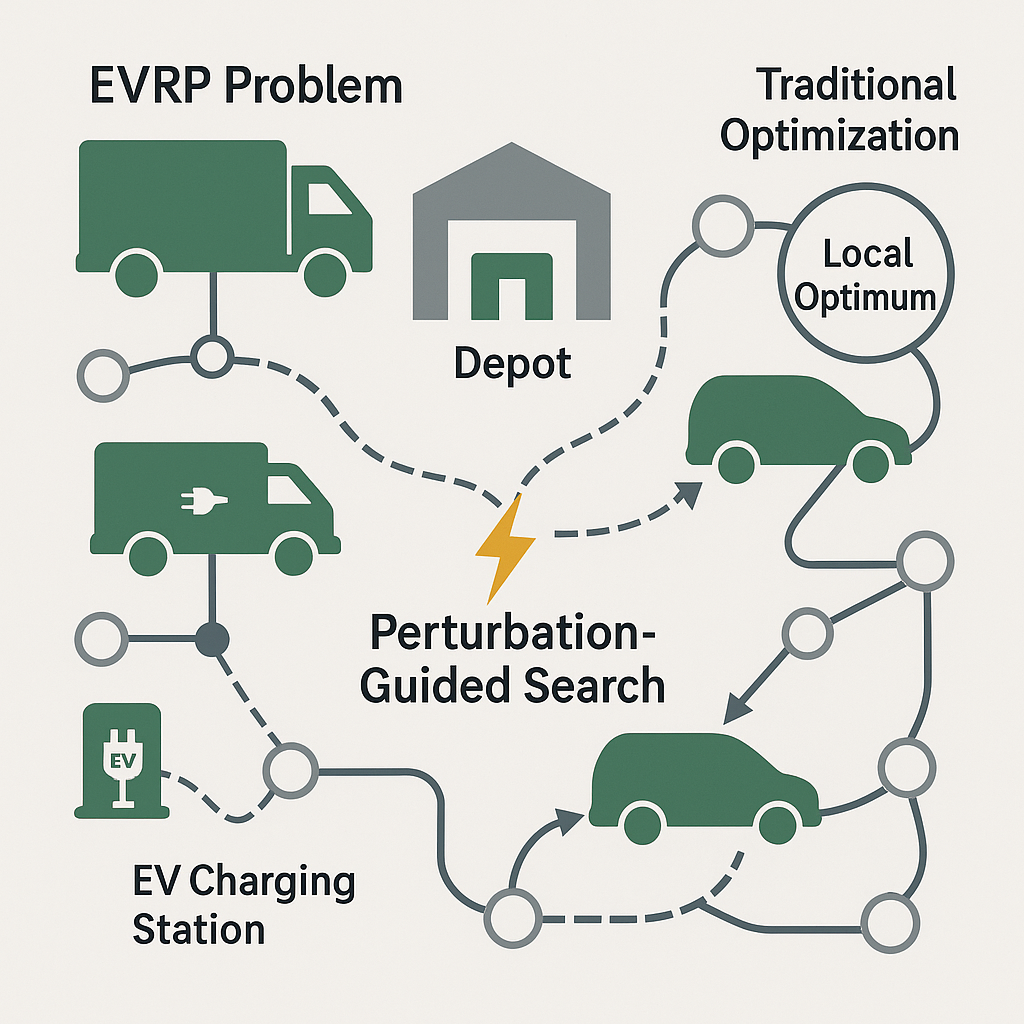
\includegraphics[width=0.8\linewidth]{image/1/main.png}
    \caption{EVRP}
    \label{fig:main}
\end{figure}

The Electric Vehicle Routing Problem (EVRP) (Fig.~\ref{fig:main}), an important extension of the classical Vehicle Routing Problem (VRP), has emerged to address the operational complexities associated with electric vehicle deployments. Unlike the VRP, which focuses solely on minimizing transportation costs under spatial and load constraints, EVRP integrates additional energy-aware considerations, including energy consumption modeling based on distance and payload, battery state-of-charge tracking, mid-route charging decisions, and strategic selection of charging stations~\cite{keskin2016partial, schiffer2017electric, schneider2014electric}.

These enhancements are essential because the deployment of EVs in logistics remains constrained by limited driving range, prolonged charging times, significant battery degradation costs, and sparse charging infrastructure~\cite{nagy2007location}. Traditional VRP models, which assume virtually unlimited range and instantaneous refueling, are therefore insufficient for planning efficient EV-based logistics operations.

To overcome these challenges, EVRP research has advanced along four key dimensions: (i) management and placement of charging stations, (ii) adoption of partial and full recharging strategies, (iii) modeling of nonlinear charging behaviors, and (iv) accommodation of heterogeneous charging station types. Efficiently solving EVRP is critical for enabling scalable and sustainable urban logistics. A feasible solution must simultaneously satisfy customer demands within tight time windows and manage dynamic battery depletion, station availability, and the complex interplay between energy consumption, route topology, and vehicle characteristics. These intertwined constraints render EVRP a highly complex, non-convex, and NP-hard problem, posing significant challenges to exact optimization methods.


\section{Motivation}

As discussed in Section~\ref{sec:broad_overview}, the Electric Vehicle Routing Problem (EVRP) presents unique operational challenges, stemming from limited battery capacities, sparse charging infrastructure, and strict payload restrictions. Traditional metaheuristic algorithms, including Genetic Algorithms (GA), Ant Colony Optimization (ACO), and Simulated Annealing (SA), have been widely applied to EVRP. However, these methods often encounter issues such as premature convergence and limited resilience in recovering from infeasible solutions.

A recent study introduced a clustering-inspired Greedy Search (GS) strategy that aims to address some of these challenges~\cite{hien2023greedy}. By clustering customer paths and greedily selecting charging stations, the GS algorithm produced high-quality initial solutions and, when embedded into a GA framework, demonstrated improved global search effectiveness.

Motivated by these findings, this project seeks to systematically extend the application of structured perturbation strategies to other metaheuristic frameworks, particularly SA and ACO. By integrating perturbation-driven diversification and domain-specific repair mechanisms, we aim to enhance these algorithms' abilities to escape local optima, maintain solution feasibility, and improve overall search robustness. This exploration not only validates the versatility of perturbation techniques across different optimization paradigms but also offers new insights into advancing EVRP solution methodologies.


\section{Aim and Objectives}

\noindent
\paragraph{Aim:}  
The aim of this project is to develop a unified perturbation-driven metaheuristic framework for solving the EVRP under energy and capacity constraints.  
By systematically integrating structured perturbation mechanisms into GA, SA, and ACO, the project seeks to enhance search diversity, improve solution robustness, and enable scalable, energy-aware urban logistics planning.

\bigskip
\noindent
\paragraph{Objectives:}
\begin{enumerate}
    \item \textbf{Conduct a comprehensive literature review:} Analyze and synthesize existing research on metaheuristic approaches for EVRP, with particular focus on the impact of perturbation strategies.
    
    \item \textbf{Implement baseline algorithms:} Develop baseline versions of GA, SA, and ACO adapted to EVRP, ensuring effective handling of energy and load constraints.
    
    \item \textbf{Design structured perturbation mechanisms:} Integrate perturbation-driven diversification into SA and ACO, leveraging insights from GA implementations, to enhance exploration and exploitation balance.
    
    \item \textbf{Develop domain-specific repair and local search strategies:} Incorporate targeted repair methods and multi-stage local search to strengthen solution feasibility and optimize route quality.
    
    \item \textbf{Perform systematic comparative experiments:} Evaluate the performance of perturbation-enhanced algorithms against baseline versions on standard EVRP benchmark datasets, measuring solution quality, computational efficiency, and robustness across multiple runs.
    
    \item \textbf{Assess scalability across problem sizes:} Test and analyze algorithm performance on both small- and large-scale EVRP instances drawn from the WCCI 2020 EVRP Competition benchmark set.
\end{enumerate}

\section{Report Structure}

The remainder of this report is organized as follows:

\begin{figure}[!h]
    \centering
    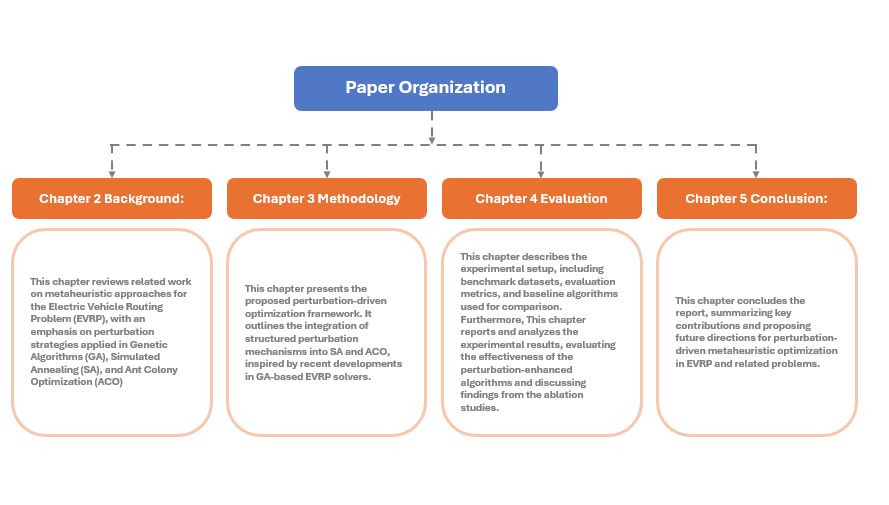
\includegraphics[width=0.8\linewidth]{image/1/paper_structure1.png}
    \caption{Paper's Structure}
    \label{fig:enter-label}
\end{figure}
\label{sec:Introduction}
\newpage

\chapter{Background}
\label{sec:Background}
\newpage
\section{The Evolution of Sustainable Logistics}
\begin{figure}[!h]
    \centering
    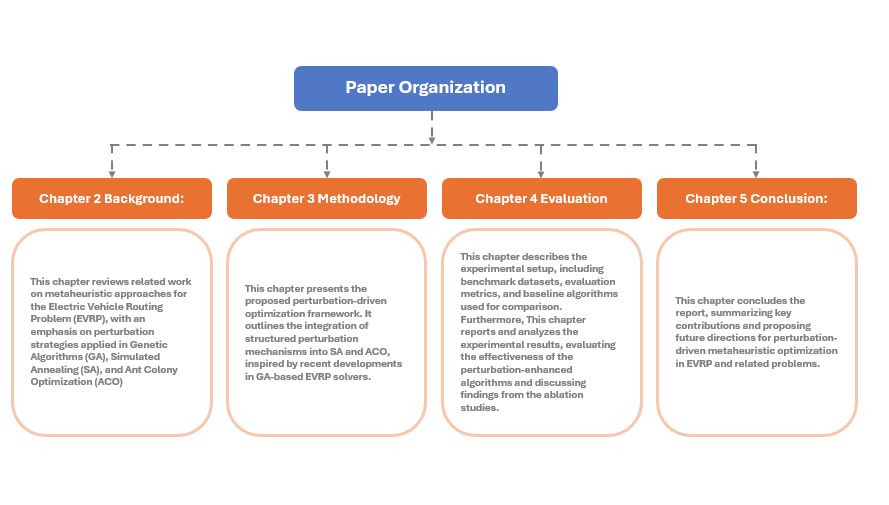
\includegraphics[width=1\linewidth]{image/1/paper_structure1.png}
    \caption{Background Structure}
    \label{fig:bg}
\end{figure}
\subsection{Environmental Concerns and CO\textsubscript{2} Emissions}

Climate change, driven primarily by the escalation of greenhouse gas emissions, has emerged as one of the most critical global challenges of the 21\textsuperscript{st} century~\cite{mccarthy2010climate}.  
The transportation sector is a major contributor, responsible for approximately 24\% of global direct CO\textsubscript{2} emissions from fuel combustion~\cite{edenhofer2015climate}.  
This significant environmental footprint has intensified pressure on governments, industries, and researchers to pursue sustainable alternatives to conventional transportation practices.

In particular, urban freight transport—dominated by logistics and delivery services—plays a disproportionate role in exacerbating air pollution within cities.  
As urbanization accelerates and e-commerce demand surges, the need for efficient yet environmentally sustainable logistics solutions has become increasingly urgent.


\subsection{Logistics Sector's Shift Towards Electrification}

In response to escalating environmental concerns and increasing regulatory pressures, the logistics sector is undergoing a fundamental transformation toward more sustainable practices.  
One of the most prominent trends is the electrification of vehicle fleets, with major logistics companies such as FedEx, UPS, and DHL making substantial investments in EVs to reduce their carbon footprint~\cite{zuo2019new, soleimani2018collection}.

EVs offer several advantages over their internal combustion engine counterparts, including zero tailpipe emissions, higher energy efficiency, and lower maintenance costs.  
These benefits align closely with corporate sustainability objectives and the growing consumer demand for greener supply chains.  
Nevertheless, integrating EVs into existing logistics operations introduces significant challenges, particularly regarding limited driving range, battery degradation, and the need for extensive charging infrastructure.


\subsection{Importance of Optimizing EV-Based Delivery Routes}

While the deployment of EVs represents a critical step toward sustainable logistics, their successful integration depends heavily on addressing their unique operational constraints.  
Unlike conventional internal combustion engine vehicles, EVs require meticulous route planning to ensure that delivery schedules are met without depleting battery reserves.  
Factors such as energy consumption rates, charging station availability, and vehicle load capacities must all be carefully considered in the routing process.

Optimizing EV-based delivery routes is therefore essential to fully realizing the environmental and economic benefits of fleet electrification.  
Effective routing minimizes the total distance traveled, reduces the frequency and duration of charging stops, and maximizes vehicle utilization, thereby enhancing the overall efficiency and sustainability of logistics operations.  
This necessity has given rise to the EVRP, a complex extension of the classical Vehicle Routing Problem, specifically tailored to account for the operational characteristics and limitations of EVs.

Addressing the EVRP through advanced optimization techniques not only reduces operational costs and environmental impact but also plays a vital role in accelerating the broader adoption of electric mobility within the logistics sector.



\section{From VRP to EVRP: Problem Transformation}

The Vehicle Routing Problem (VRP) is a classical combinatorial optimization problem concerned with determining optimal routes for a fleet of vehicles to service a set of customers from a central depot.  
Each customer must be visited exactly once, and the total travel distance or cost must be minimized, subject to constraints such as vehicle load capacity and maximum route duration.

While extensively studied, the classical VRP does not account for energy-related limitations.  
As electric vehicles (EVs) increasingly replace traditional internal combustion engine (ICE) vehicles, the routing paradigm must be adapted to accommodate additional constraints such as battery capacity, energy consumption per route segment, and the availability and location of charging stations.  
This gives rise to the Electric Vehicle Routing Problem (EVRP), which generalizes the VRP by embedding energy-awareness into the model.

Formally, let $G = (V, E)$ denote a complete directed graph, where $V = \{v_0, v_1, \dots, v_n\}$ represents the set of nodes, with $v_0$ corresponding to the depot and $\{v_1, \dots, v_n\}$ the customer locations.  
Each edge $(i, j) \in E$ is associated with a travel cost $c_{ij}$ and an energy consumption value $e_{ij}$.  
Each EV has a battery capacity $Q$ and may recharge at designated charging stations $R \subset V$.

A feasible route $r = \{v_0, v_{i_1}, v_{i_2}, \dots, v_{i_k}, v_0\}$ must satisfy the following constraints:

\begin{itemize}
    \item \textbf{Visit constraint}: Each customer node $v_i \in V \setminus \{v_0\}$ must be visited exactly once.
    \item \textbf{Capacity constraint}: The total demand served along a route must not exceed the vehicle's load capacity.
    \item \textbf{Energy constraint}: The cumulative energy consumption along any route segment between recharges must not exceed the battery capacity $Q$:
    \[
        \sum_{(i, j) \in r'} e_{ij} \leq Q
    \]
    where $r'$ denotes any sub-route between two recharge points.
    \item \textbf{Recharge feasibility}: Vehicles may recharge at designated nodes $v_j \in R$, where the battery is fully replenished.
\end{itemize}

Compared to the classical VRP, the inclusion of energy-aware constraints significantly increases the solution space complexity.  
Routing algorithms must not only determine customer visiting sequences but also strategically plan recharge stops, optimize energy usage, and account for additional factors such as vehicle load and terrain elevation.

Moreover, EVRP introduces the possibility of infeasible partial solutions—routes that may be cost-optimal but invalid due to battery depletion before reaching a charging station.  
This necessitates the integration of robust feasibility checking and solution repair mechanisms within optimization procedures.

As an extension of the VRP, the EVRP additionally requires the planning of charging station visits alongside customer servicing (Fig.~\ref{fig:vs}).  
Since the classical VRP is already known to be NP-hard, the EVRP, as its generalization, remains strongly NP-hard.  
Furthermore, the incorporation of energy and recharge constraints, as outlined above, renders the problem even more challenging to solve.

\begin{figure}
    \centering
    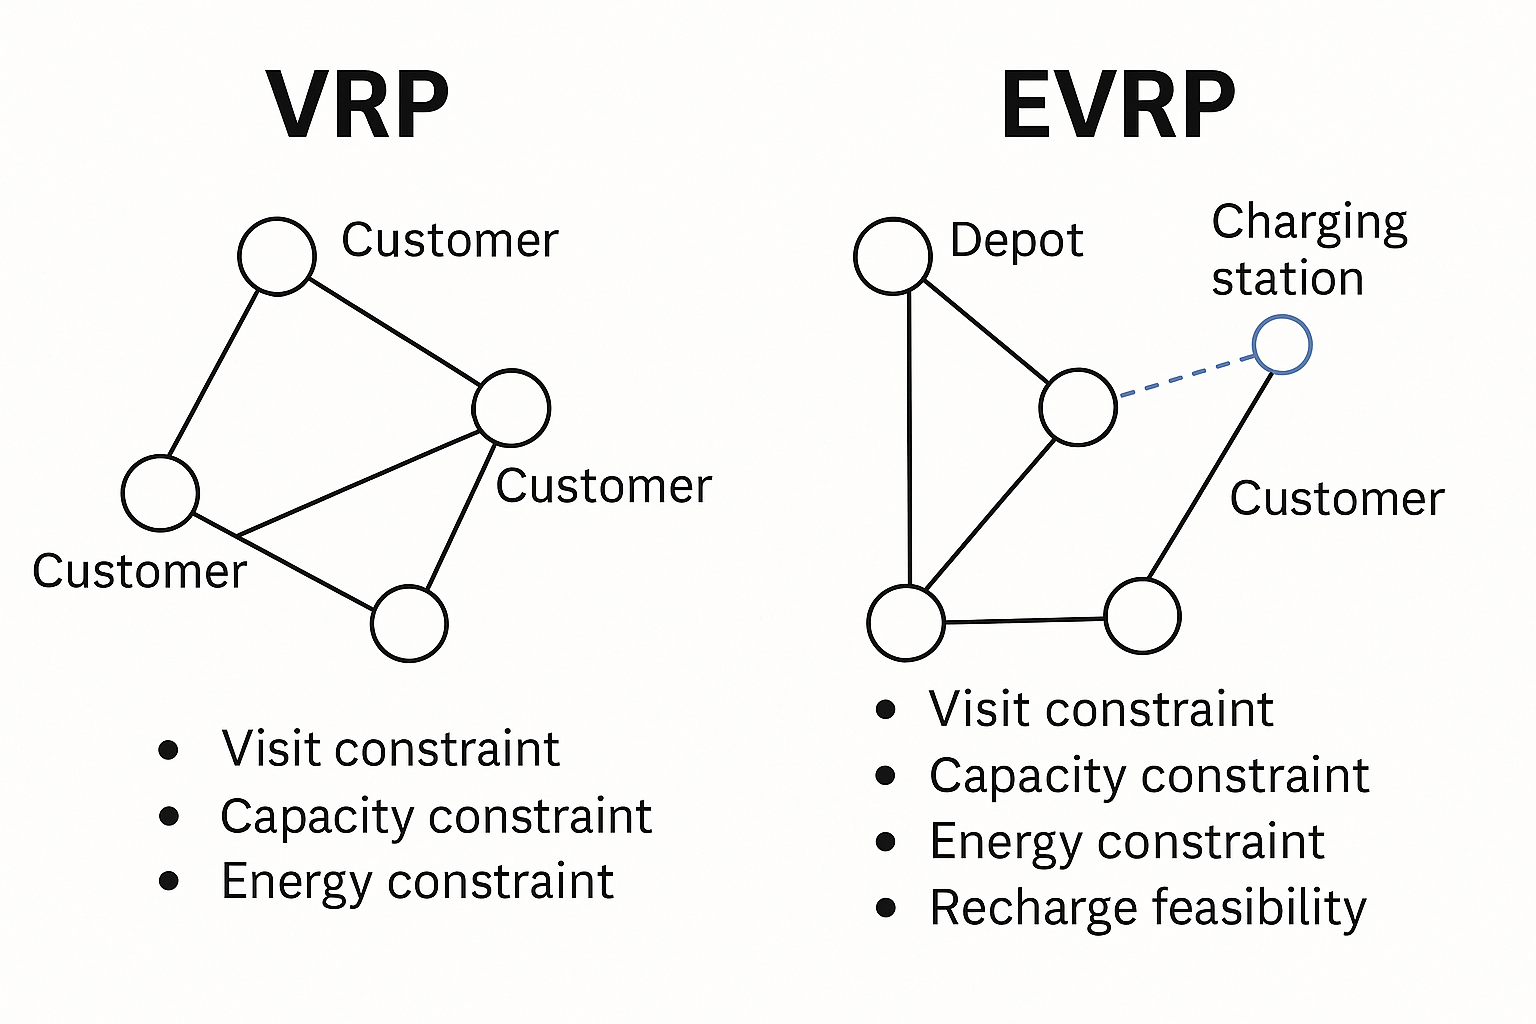
\includegraphics[width=1\linewidth]{image/2/Logistics Optimization_ VRP vs EVRP.png}
    \caption{VRP vs. EVRP}
    \label{fig:vs}
\end{figure}


\subsection{Problem Definition of the Electric Vehicle Routing Problem}

The Electric Vehicle Routing Problem involves determining a set of vehicle routes, where each route serves a subset of customer nodes and must both start and end at a designated depot~\cite{schiffer2017electric}.  
The primary objective is to optimize route planning for electric vehicles by minimizing a given cost function, typically the total travel distance, while satisfying operational constraints associated with vehicle limitations.

The EVRP is based on the following key assumptions~\cite{kucukoglu2021electric}:
\begin{itemize}
    \item Each route begins and ends at the depot.
    \item Each customer node is visited exactly once by exactly one vehicle.
    \item Vehicles are allowed to visit charging stations en route to replenish their battery.
    \item Multiple vehicles may use the same charging station without restriction.
    \item The distances between all nodes and the locations of charging stations are known and fixed.
    \item The battery level of each vehicle must remain within the bounds of zero and its maximum capacity at all times during operation.
    \item After visiting a charging station, the vehicle's battery is assumed to be fully recharged.
\end{itemize}

Compared to the classical Vehicle Routing Problem, the EVRP introduces additional complexities by explicitly modeling energy constraints, necessitating strategic planning of charging station visits alongside customer servicing.

\subsubsection{Current Classifications of EVRP Models}

\paragraph{Based on Objective Functions}

Existing EVRP models can be categorized according to their primary optimization objectives.  
A large body of work, including studies by Chen et al.~\cite{chen2016electric}, Cubides et al.~\cite{cubides2019electric}, Catay and Keskin~\cite{ccatay2017impact}, and Ding et al.~\cite{ding2015conflict}, focuses on minimizing the total travel distance, reflecting the traditional VRP objective.

Other studies, such as those by Abdulaal et al.~\cite{abdulaal2016solving}, Ceselli et al.~\cite{ceselli2021branch}, and Felipe et al.~\cite{felipe2014heuristic}, prioritize minimizing total charging cost or total charging time, acknowledging the practical impact of prolonged recharging in EV operations.

Additionally, a third group of research, including the works of Abdallah et al.~\cite{abdallah2020electric}, Barco et al.~\cite{barco2017optimal}, and Basso et al.~\cite{basso2019energy, basso2021electric}, adopts total energy consumption as the main optimization objective, reflecting the growing importance of energy efficiency in sustainable logistics.

\paragraph{EVRP Constraints}

Compared to the classical Vehicle Routing Problem, the Electric Vehicle Routing Problem introduces additional constraints, with energy management during recharging being a particularly critical aspect.  
Charging constraints in EVRP models are generally classified into two categories: full charging and partial charging strategies.

Under the \textbf{full charging} assumption, vehicles must leave charging stations with fully replenished batteries.  
This simplifies energy tracking but may increase charging times and lead to potential inefficiencies.  
Representative studies adopting this assumption include Ghobadi et al.~\cite{ghobadi2021multi}, Goeke and Schneider~\cite{goeke2015routing}, Granada-Echeverri et al.~\cite{granada2020electric}, Hiermann et al.~\cite{hiermann2016electric}, Jia et al.~\cite{jia2021bilevel}, and Keskin et al.~\cite{keskin2016partial}.

Conversely, \textbf{partial charging} strategies allow vehicles to leave charging stations with incomplete recharges, depending on operational needs and time constraints.  
Partial charging offers greater routing flexibility and can enhance overall system efficiency, especially under nonlinear charging dynamics or tight delivery windows.  
Notable works adopting this approach include Bruglieri et al.~\cite{bruglieri2017three}, Futalef et al.~\cite{futalef2020evolutionary}, Karakatic~\cite{karakativc2021optimizing}, Kouider et al.~\cite{kouider2018constructive}, and Lee et al.~\cite{lee2021exact}.

In summary, the choice of optimization objective and charging strategy significantly influences EVRP model design, solution complexity, and applicability to real-world logistics scenarios.


\section{Approaches to Solving EVRP}

As an extension of the classical VRP, which is known to be NP-hard, the EVRP is similarly classified as a strongly NP-hard problem~\cite{desaulniers2016exact,ferro2018optimization,roberti2016electric}.  
Solving the EVRP requires algorithms capable of addressing not only the underlying combinatorial complexity but also the additional operational constraints introduced by limited battery capacity and recharging requirements.  
Over the years, researchers have proposed a wide range of solution techniques, which can be broadly categorized into three main groups: exact methods, heuristic strategies, and metaheuristic frameworks.

\subsection{Exact Methods for Solving EVRP}

Exact methods aim to compute globally optimal solutions by formulating the EVRP within a rigorous mathematical programming framework.  
Among these, Mixed Integer Programming (MIP) models are most commonly employed, where routing decisions, energy consumption tracking, and recharging operations are represented by a combination of binary and continuous variables.  
However, the integration of energy constraints greatly enlarges the solution space, making pure MIP formulations computationally impractical for large-scale instances.

To enhance tractability, advanced strategies such as Branch-and-Bound, Branch-and-Cut, and Branch-and-Price have been developed.  
Branch-and-Cut approaches strengthen linear programming relaxations via the addition of valid inequalities, while Branch-and-Price utilizes dynamic column generation to manage exponentially large route sets more efficiently.  
Hybrid Branch-Price-and-Cut frameworks, which combine these two ideas, currently represent the state-of-the-art among exact EVRP solvers.  
Moreover, Set Partitioning formulations are sometimes adopted, particularly when feasible energy-valid paths can be precomputed.

Notable examples of exact solution approaches include Tahami et al.~\cite{tahami2020exact}, who applied a Branch-and-Bound algorithm to standard EVRP instances, and Lee et al.~\cite{lee2021exact}, who developed a Branch-and-Price method to optimally solve EVRP variants involving nonlinear charging time models.

Despite their theoretical rigor and ability to guarantee optimality, exact methods face severe scalability challenges.  
Solution times increase exponentially with the number of customers, charging stations, or additional modeling complexities such as partial charging, heterogeneous fleets, or time windows.  
Consequently, exact methods are primarily restricted to small- or medium-sized instances and are mainly used for benchmarking heuristic and metaheuristic approaches.

In addition to bespoke academic solvers, commercial optimization software such as CPLEX~\cite{hulagu2019multiple,keskin2019electric} and GUROBI~\cite{moghaddam2015partially,schiffer2017electric} have also been employed for solving specific EVRP formulations.  
However, even with these powerful solvers, handling large-scale EVRP instances remains a substantial computational challenge.



\subsection{Heuristic Methods for Solving EVRP}

Heuristic methods for solving the Electric Vehicle Routing Problem (EVRP) are based on empirical strategies designed to quickly generate feasible, though not necessarily optimal, solutions.  
They are generally classified into two categories: constructive heuristics and improvement heuristics.

Constructive heuristics, such as nearest neighbor and savings-based approaches, incrementally build a feasible solution by inserting customer nodes and charging stations while satisfying energy and capacity constraints.  
Greedy Recharging Heuristic (GRH) strategies further extend these methods by incorporating energy-aware selection criteria, considering not only travel distance but also residual battery levels and proximity to charging infrastructure~\cite{felipe2014heuristic,schiffer2018adaptive,schneider2014electric}.

Improvement heuristics focus on enhancing an existing solution through local search operations.  
Common neighborhood operators include swap, relocate, and 2-opt or 3-opt moves, which aim to reduce total route cost while maintaining feasibility with respect to energy constraints.  
To address constraint violations arising during local search, specialized repair mechanisms are often integrated into the optimization process.

An alternative to heuristic-based charging station insertion is the use of forward labeling algorithms based on dynamic programming principles.  
Labeling methods systematically extend partial routes from the depot, inserting charging stations as necessary to maintain feasibility concerning battery capacity and time windows.  
By progressively constructing feasible paths, these algorithms can identify optimal recharge patterns for a given customer sequence.  
Although labeling algorithms are generally more computationally intensive than heuristic insertion methods, they often yield higher-quality solutions when computational resources permit.  
The charging station insertion problem, closely related to the resource-constrained shortest path problem, is also known to be strongly NP-hard~\cite{hiermann2016electric}.

Despite their computational efficiency, heuristic methods have inherent limitations.  
They are prone to premature convergence to suboptimal solutions, particularly in large-scale or highly constrained instances, and their manually crafted rules may lack adaptability to different EVRP variants, such as models with partial recharging or heterogeneous fleets.

Nevertheless, due to their low computational overhead, heuristic approaches remain valuable for quickly producing high-quality initial solutions, providing effective warm starts for metaheuristic algorithms, and serving as baselines for comparative evaluations.

\subsection{Metaheuristic Methods}

Metaheuristics are high-level strategies that guide local or global search procedures using problem-agnostic frameworks. They strike a balance between solution quality and scalability, making them particularly suitable for real-world EVRP instances.

\paragraph{Genetic Algorithms}

Genetic Algorithms (GAs) are population-based metaheuristic optimization techniques inspired by the principles of natural evolution. In the context of EVRP, GAs evolve a population of candidate solutions (routes) over successive generations to progressively enhance solution quality while satisfying energy constraints~\cite{abdallah2020electric}.

At each generation, the algorithm maintains a population of individuals, where each individual represents a feasible or partially feasible sequence of customer visits and recharging decisions. The evolutionary process consists of three primary operators: selection, crossover, and mutation.

\textbf{Selection:} A subset of parent solutions is selected from the current population based on fitness, typically evaluated according to the total route cost or energy consumption. Common selection strategies include tournament selection and roulette-wheel selection.

\textbf{Crossover:} Two parent solutions are combined to produce offspring by exchanging subsequences of customer visits and recharge decisions. In EVRP-specific adaptations, crossover operators are often designed to preserve energy-feasible segments or prioritize recharging station placements.

\textbf{Mutation:} Offspring solutions undergo random perturbations to maintain diversity and avoid premature convergence. Mutation operations may include swapping two customer nodes, inserting or removing a recharge station, or reversing a subsequence, with energy constraints checked or repaired as necessary.

After crossover and mutation, a new population is generated. The best-performing individuals may be retained through elitism to ensure steady improvement. The evolutionary cycle continues until a predefined stopping criterion is met, such as a maximum number of generations or convergence of solution quality.

Throughout the search process, energy feasibility checking and repair heuristics are integrated to ensure that candidate solutions remain valid under EVRP-specific operational constraints~\cite{abdulaal2016solving}.

\begin{algorithm}[H]
\caption{Genetic Algorithm for EVRP}
\begin{algorithmic}[1]
\State Initialize population $P$ with $N$ feasible or partially feasible routes
\While{stopping criterion not met}
    \ForAll{individuals in $P$}
        \State Evaluate fitness
    \EndFor
    \State Select parent solutions based on fitness
    \State Apply crossover to generate offspring
    \State Apply mutation to offspring
    \ForAll{offspring}
        \If{infeasible}
            \State Repair solution
        \EndIf
    \EndFor
    \State Form new population $P'$ by selecting the best individuals (elitism)
    \State $P \gets P'$
\EndWhile
\State \Return Best solution found
\end{algorithmic}
\end{algorithm}

Genetic Algorithms provide a flexible and robust framework for exploring the complex and multimodal solution space of EVRP, effectively balancing exploration and exploitation through stochastic evolutionary operators.


\paragraph{Simulated Annealing}

Simulated Annealing (SA) is a single-solution-based metaheuristic inspired by the physical annealing process in metallurgy, where controlled cooling enables a material to reach a low-energy crystalline structure. In the context of EVRP, SA explores the solution space by iteratively perturbing a current solution and probabilistically accepting candidate solutions based on both solution quality and a dynamically decreasing temperature parameter~\cite{erdougdu2020distance}.

At each iteration, the current solution is modified using a neighborhood operator to generate a new candidate solution. The acceptance decision for the new solution depends on a probability function that considers both the change in objective function value and the current temperature. Worse solutions may be accepted with a certain probability, allowing the algorithm to escape local minima during the early stages of the search.

Initially, the temperature is set to a high value to encourage exploration across the solution landscape. As the search progresses, the temperature is gradually reduced according to a cooling schedule, typically following a geometric decay pattern, where each new temperature is a fraction of the previous one. The rate of temperature decrease controls the balance between exploration and exploitation.

Energy feasibility is maintained during the generation of neighbor solutions, with repair heuristics applied when necessary to ensure that battery constraints and recharge station feasibility are satisfied. Typical neighborhood moves in EVRP-specific SA implementations include customer swap, insertion or removal of recharge stops, subsequence reversal, and reassignment of charging stations.

The algorithm continues until a predefined termination condition is met, such as reaching a minimum temperature threshold or a maximum number of iterations. By accepting uphill moves early in the search and gradually reducing the acceptance probability, Simulated Annealing effectively balances diversification and intensification, making it well-suited for the rugged and multimodal solution landscapes characteristic of EVRP~\cite{ghobadi2021multi}.

\begin{algorithm}[H]
\caption{Simulated Annealing for EVRP}
\begin{algorithmic}[1]
\State Initialize temperature $T$ and generate initial solution $s_{\text{curr}}$
\State Set $s_{\text{best}} \gets s_{\text{curr}}$
\While{stopping criterion not met}
    \State Generate a neighbor solution $s_{\text{new}}$ from $s_{\text{curr}}$
    \If{$s_{\text{new}}$ is better than $s_{\text{curr}}$}
        \State Accept $s_{\text{new}}$ as the new current solution
    \Else
        \State Accept $s_{\text{new}}$ with a probability dependent on $T$
    \EndIf
    \If{$s_{\text{new}}$ is better than $s_{\text{best}}$}
        \State Update $s_{\text{best}} \gets s_{\text{new}}$
    \EndIf
    \State Decrease temperature $T$ according to the cooling schedule
\EndWhile
\State \Return $s_{\text{best}}$
\end{algorithmic}
\end{algorithm}


\paragraph{Ant Colony Optimization}

Ant Colony Optimization (ACO) is a population-based metaheuristic inspired by the foraging behavior of ants, where pheromone trails guide the discovery of shortest paths between food sources and their nest. In the context of EVRP, ACO models candidate routes as paths constructed probabilistically based on artificial pheromone intensities and heuristic information that accounts for both travel distance and energy feasibility~\cite{jia2021bilevel, mavrovouniotis2019parallel,mavrovouniotis2018ant}.

During each iteration, a colony of artificial ants builds feasible routes by moving from node to node according to a transition probability. The probability of selecting the next node depends on two key factors: the intensity of the pheromone trail and the heuristic desirability of the move, typically defined as the inverse of distance or estimated energy consumption. Parameters are introduced to control the relative influence of pheromone strength and heuristic visibility. Feasibility considerations, such as battery capacity and charging station availability, constrain the set of nodes available for selection at each step~\cite{mao2020electric}.

Once all ants have completed their routes, pheromone trails are updated through a combination of evaporation and reinforcement. Pheromone evaporation prevents premature convergence by gradually reducing the strength of all trails, while reinforcement increases the pheromone levels on paths associated with high-quality solutions. In many EVRP-specific adaptations, elitist strategies are employed where the best solutions deposit additional pheromones to accelerate convergence toward promising regions of the solution space.

To enhance performance, energy-aware heuristic adjustments, local search refinements, and feasibility repair operations are often integrated into the basic ACO framework. These enhancements address the complex interactions between routing and recharging decisions that are characteristic of EVRP~\cite{meng2020route}.

Through iterative learning and probabilistic exploration, ACO effectively balances diversification and intensification, making it a robust and flexible approach for solving EVRP instances, particularly when facing scalability challenges or complex constraint landscapes~\cite{zhao2020distribution,zhao2020distribution}.

\begin{algorithm}[H]
\caption{Ant Colony Optimization for EVRP}
\begin{algorithmic}[1]
\State Initialize pheromone levels on all edges
\While{stopping criterion not met}
    \ForAll{ants}
        \State Construct a feasible route based on pheromone and heuristic information
    \EndFor
    \State Apply local search or repair mechanisms if necessary
    \State Update pheromone trails based on the quality of constructed routes
    \State Apply pheromone evaporation to all edges
\EndWhile
\State \Return Best solution found
\end{algorithmic}
\end{algorithm}

\subsection{Comparison of Metaheuristic Perturbation Mechanisms}

Although Genetic Algorithms (GA), Simulated Annealing (SA), and Ant Colony Optimization (ACO) are all metaheuristic frameworks, they incorporate fundamentally different mechanisms for introducing perturbations into the solution space~\cite{kumbharana2013comparative}.

In GA, perturbations arise primarily through crossover and mutation operations. Crossover creates large-scale structural perturbations by recombining segments from two parent solutions, promoting exploration across diverse regions of the search space. Mutation introduces smaller, localized changes, such as swapping customer nodes or inserting charging stations, thereby maintaining diversity and preventing premature convergence. Additionally, the strength of perturbation can be dynamically tuned through mutation rates or customized crossover designs. Selection pressure, often governed by fitness-proportional selection or tournament schemes, further shapes the global exploration-exploitation balance. Overall, GA integrates both structured (crossover) and random (mutation) perturbations, combining global and local search dynamics~\cite{ansari2015comparison}.

In SA, perturbations are introduced at the level of single-solution modifications using neighborhood operators. Each move, such as a customer swap, node relocation, or subsequence reversal, induces a localized perturbation around the current solution. The acceptance of perturbations is probabilistic and temperature-dependent: at high temperatures, worse solutions may be accepted to escape local minima ("controlled randomness"), while at lower temperatures, the acceptance becomes more selective, favoring quality-improving moves. Hence, SA primarily conducts localized, temperature-adaptive perturbations, dynamically shifting from exploration to exploitation during the cooling process. The design and diversity of move operators are also crucial for maintaining effective search behavior.

In ACO, perturbation is embedded implicitly within the stochastic solution construction process. Each ant constructs a solution probabilistically based on pheromone levels (exploitation) and heuristic desirability (exploration), introducing inherent variability across ants. Unlike GA and SA, where perturbation modifies existing solutions, ACO builds new solutions from scratch at each iteration. The evaporation of pheromones further acts as a global perturbation mechanism, preventing path stagnation and encouraging exploration of underutilized routes~\cite{comert2023new}.

From a perturbation perspective, GA employs both global and local operators to maintain balance, SA relies on localized moves with an adaptive acceptance probability shaped by the cooling schedule, while ACO injects stochasticity at the construction phase and dynamically adjusts global learning via pheromone updates~\cite{li2022overview}. Each framework embodies an exploration-exploitation strategy, tailored to navigating the constraint-laden solution landscape of the EVRP~\cite{sabet2022green,matijevic2023metaheuristic}.




\newpage

\chapter{Methodology}
\newpage
\label{sec:Methodology}

\section{Overview}
The overall workflow of the project is illustrated in Figure~\ref{fig:framework}.

\begin{figure}[!h]
    \centering
    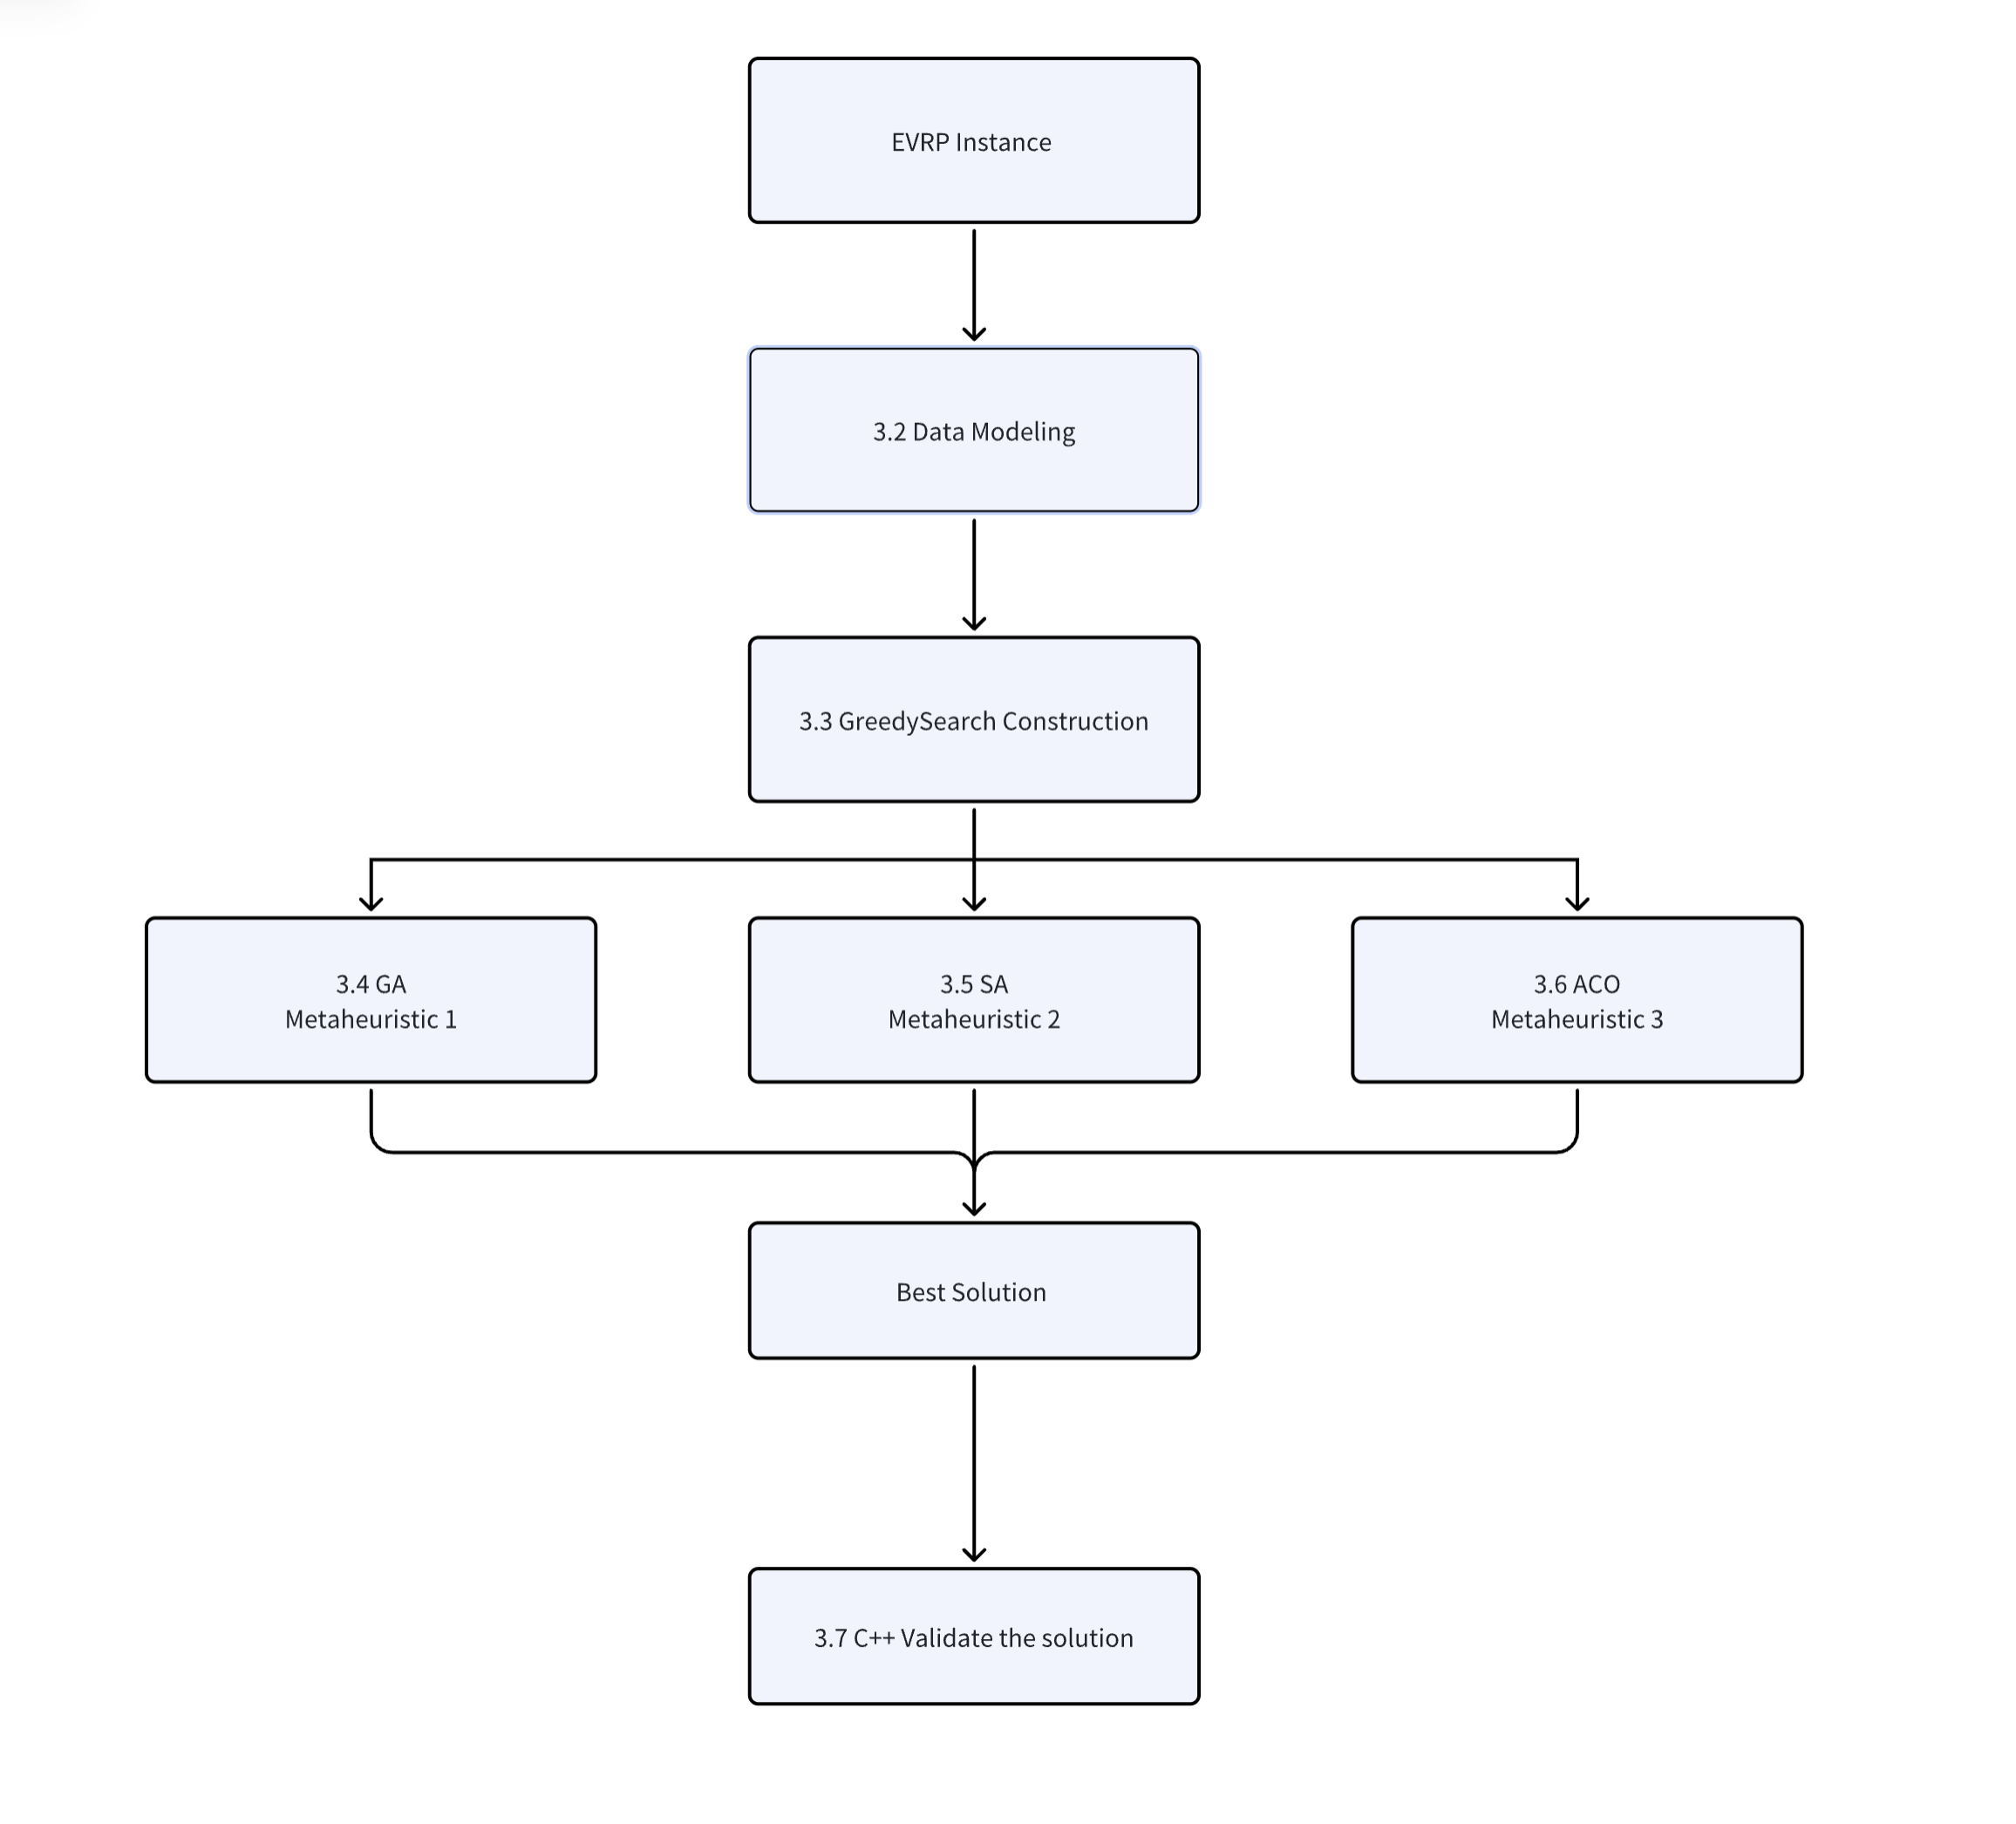
\includegraphics[width=0.7\linewidth]{image/3/framework.png}
    \caption{Overall framework of the proposed solution.}
    \label{fig:framework}
\end{figure}

The process begins with the selection of an EVRP (Electric Vehicle Routing Problem) instance.  
In Section~\ref{sec:data_modeling}, the data is modeled to represent the problem environment, including customer locations, charging stations, and vehicle constraints.  
Next, in Section~\ref{sec:greedy_search}, an initial feasible solution is constructed using a Greedy Search strategy to provide a starting point for further optimization.  
Subsequently, three different metaheuristic approaches are applied separately: Genetic Algorithm in Section~\ref{sec:ga}, Simulated Annealing in Section~\ref{sec:sa}, and Ant Colony Optimization in Section~\ref{sec:aco}.  
Each method searches for high-quality solutions independently.  
Afterward, the best solution among the three is selected.  
Finally, in Section~\ref{sec:cpp_validation}, a C++ program is used to validate the correctness and feasibility of the obtained solution.




\section{Problem Formulation}

The Electric Vehicle Routing Problem (EVRP) considered in this project is formulated on a complete undirected graph \( G = (V, E) \), where \( V \) denotes the set of all nodes and \( E \) represents the set of edges connecting pairs of nodes. The node set \( V \) is partitioned into three disjoint subsets: the depot \( D \), the set of customers \( C \), and the set of charging stations \( S \), satisfying:
\[
V = D \cup C \cup S
\]

Each edge \( (i, j) \in E \) is associated with a non-negative Euclidean distance \( d_{ij} \) and an energy consumption \( e_{ij} = h \times d_{ij} \), where \( h > 0 \) denotes the energy consumption rate per unit distance.

A homogeneous fleet of vehicles is available, each characterized by:
\begin{itemize}
    \item A maximum load capacity \( C \) for carrying customer demands.
    \item A maximum battery capacity \( Q \) limiting travel between recharges.
\end{itemize}

Each customer node \( i \in C \) has a demand \( q_i \geq 0 \). Charging stations \( S \) and the depot \( D \) offer opportunities for full battery replenishment.

The goal of EVRP is to construct a set of routes, each starting and ending at the depot, while minimizing total travel distance and satisfying the following constraints:

\begin{itemize}
    \item \textbf{Service constraint}: Each customer must be visited exactly once by a vehicle.
    \item \textbf{Capacity constraint}: The total demand served in a route must not exceed vehicle capacity \( C \).
    \item \textbf{Energy constraint}: The cumulative energy consumed between consecutive recharge opportunities must not exceed battery capacity \( Q \).
\end{itemize}

Formally, the objective is:
\[
\min \sum_{k \in K} \sum_{(i, j) \in r_k} d_{ij}
\]
where \( r_k \) is the sequence of nodes visited by vehicle \( k \).

This formulation captures the combined logistical (load) and energy (battery) constraints, making EVRP a complex and realistic extension of the classical Vehicle Routing Problem (VRP).

\bigskip

\section{Data Representation and Problem Setup}
\label{sec:data_modeling}

To enable computational implementation of the above formulation, the EVRP instance is structured into a set of data representations as follows.

Each node \( i \in V \) is modeled with attributes:
\begin{itemize}
    \item Unique identifier \( \text{id}_i \).
    \item Coordinates \( (x_i, y_i) \) in two-dimensional Euclidean space.
    \item Node type: customer, charging station, or depot.
    \item Demand \( q_i \geq 0 \) (positive for customers, zero otherwise).
\end{itemize}

The Euclidean distance between nodes \( i \) and \( j \) is calculated as:
\[
d_{ij} = \sqrt{(x_i - x_j)^2 + (y_i - y_j)^2}
\]
and the corresponding energy consumption is:
\[
e_{ij} = h \times d_{ij}
\]
with \( h \) specified for each problem instance.

The full problem setup includes:
\begin{itemize}
    \item Customer set \( C \) and their demands.
    \item Charging station set \( S \).
    \item Depot node \( D \).
    \item Distance matrix \( \{ d_{ij} \} \) and energy matrix \( \{ e_{ij} \} \).
    \item Vehicle parameters: capacity \( C \) and battery limit \( Q \).
\end{itemize}

To accelerate metaheuristic search procedures, a precomputed nearest-neighbor list \( \mathcal{N}(i) \) for each node is optionally constructed, sorted by ascending distance.

\bigskip
\noindent\textbf{Solution Validation}

Any proposed solution must satisfy:
\begin{itemize}
    \item Each customer is visited exactly once.
    \item No route exceeds the vehicle's load capacity.
    \item No route exceeds the battery capacity between recharge points.
\end{itemize}
Feasibility checks are systematically enforced to ensure all evaluated solutions are valid under the problem constraints.


\section{Initial Solution Construction: Greedy Search Algorithm}
\label{sec:greedy_search}

To construct an initial feasible solution for the Electric Vehicle Routing Problem (EVRP), a multi-stage greedy heuristic is employed.  
The method progressively builds capacity-aware and energy-feasible routes by clustering customers, inserting depots and charging stations when necessary, and applying local optimization. The procedure consists of the following stages:

\subsection{Problem Setup}

The \texttt{GreedySearch} algorithm is initialized with a \texttt{Problem} instance, which provides access to customer nodes, charging stations, the depot, and global parameters such as vehicle load capacity \( C \) and battery capacity \( Q \).

To accelerate the search process, two nearest-neighbor matrices are precomputed:
\begin{itemize}
    \item \textbf{Customer-Customer Nearest Neighbor Matrix}: Facilitates fast clustering of customers.
    \item \textbf{Node-Station Nearest Neighbor Matrix}: Enables rapid identification of charging stations for energy management.
\end{itemize}

\subsection{Customer Clustering}

An initial set of tours is constructed by greedily clustering customers based on spatial proximity and vehicle load constraints:
\begin{itemize}
    \item Customers are randomly shuffled to introduce initialization diversity.
    \item A center customer is selected to seed each tour, with nearby customers added sequentially without exceeding capacity \( C \).
    \item If the maximum number of vehicles is reached, any remaining unassigned customers are appended to the last tour.
    \item Empty tours are padded if necessary to match the fleet size.
\end{itemize}

\subsection{Capacity Balancing}

To improve fleet utilization, customers from overloaded tours are reallocated to underloaded ones whenever possible, prioritizing proximity and load balancing.

\subsection{Local Search Optimization (2-Opt)}

Each tour undergoes local refinement via the classical 2-opt heuristic:
\begin{itemize}
    \item Non-adjacent edges are iteratively swapped to reduce total travel distance.
    \item Optimization continues until no further improvements are found.
\end{itemize}

\subsection{Depot Insertion}

Depot nodes are inserted dynamically to maintain vehicle load feasibility:
\begin{itemize}
    \item When cumulative load threatens to exceed \( C \), a depot is inserted to allow reloading.
    \item Depot positions are greedily optimized to minimize additional travel distance.
\end{itemize}

\subsection{Charging Station Insertion and Optimization}

Energy constraints are enforced by strategically inserting charging stations:
\begin{itemize}
    \item When insufficient energy remains to reach the next node, the nearest feasible charging station is inserted.
    \item Greedy replacements are attempted to substitute inefficient charging stations with better alternatives without violating feasibility.
\end{itemize}

\subsection{Solution Finalization}

The finalized tours are encapsulated into a \texttt{Solution} object, ensuring compliance with both load and energy constraints.  
This initial solution provides a high-quality, feasible starting point for subsequent metaheuristic optimization stages.

\bigskip
This multi-stage greedy construction strategy ensures that the initial solution is not only feasible but also sufficiently optimized to accelerate convergence of higher-level algorithms such as GA, SA, and ACO.





\section{Metaheuristic Optimization: Greedy-Search Genetic Algorithm}
\label{sec:ga}
\begin{figure}[!h]
    \centering
    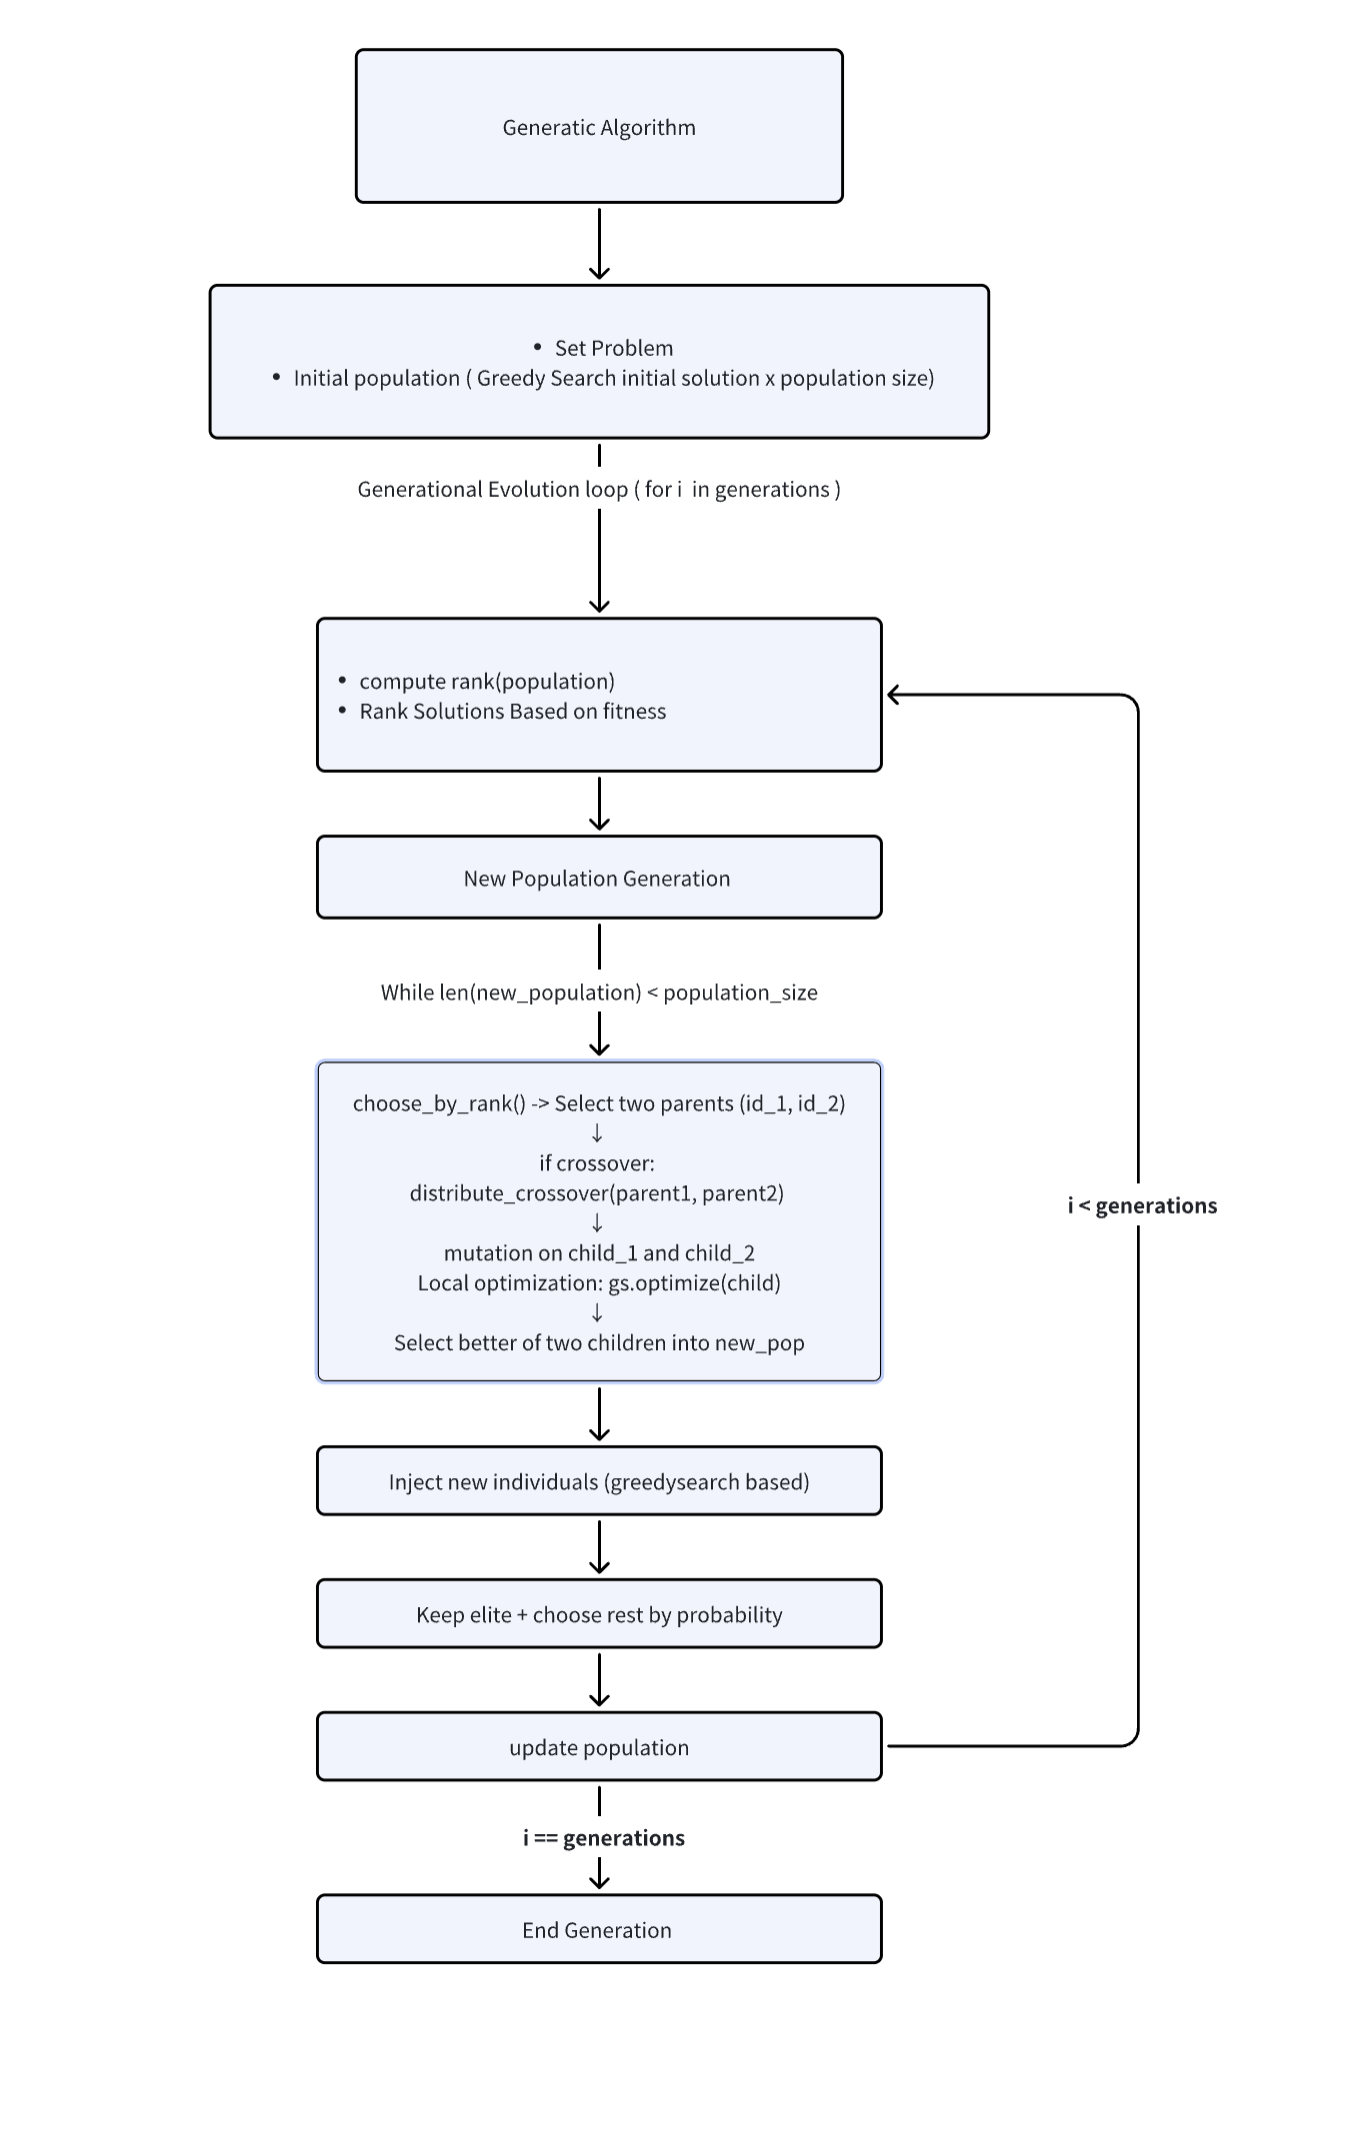
\includegraphics[width=0.7\linewidth]{image/3/gaflow.png}
    \caption{GA's flow chart}
    \label{fig:gaflow}
\end{figure}
Furthermore, the GA is developed based on this work~\cite{hien2023greedy}(Fig.~\ref{fig:gaflow}). This method integrates evolutionary exploration with domain-specific greedy optimization to achieve a balance between diversification and intensification.  
The optimization process is organized into the following stages:

First, the initial population is generated by applying greedy clustering and local search to randomized customer assignments, ensuring both feasibility and diversity.  
An elitist selection strategy is employed, preserving a fixed proportion of top-performing individuals while sampling the remainder via fitness-proportional probabilities to promote exploration.

Offspring are created through a distribute crossover operator, reallocating customer subsets between two parents while preserving route feasibility.  
Mutation is applied probabilistically to offspring, dynamically selecting among heavy mutation (HMM), heavy swap mutation (HSM), and random swap mutation operators according to a cosine-decay schedule, gradually shifting focus from exploration to exploitation.

Each offspring undergoes greedy local repair to correct constraint violations and improve solution quality.  
To mitigate premature convergence, a portion of each generation is periodically refreshed by injecting new greedy-optimized individuals.

The evolutionary process is iterated for a fixed number of generations, continuously updating the best solution found and dynamically adjusting operator selection intensity according to progress.

\section{Metaheuristic Optimization: Simulated Annealing}
\label{sec:sa}
\begin{figure}[!h]
    \centering
    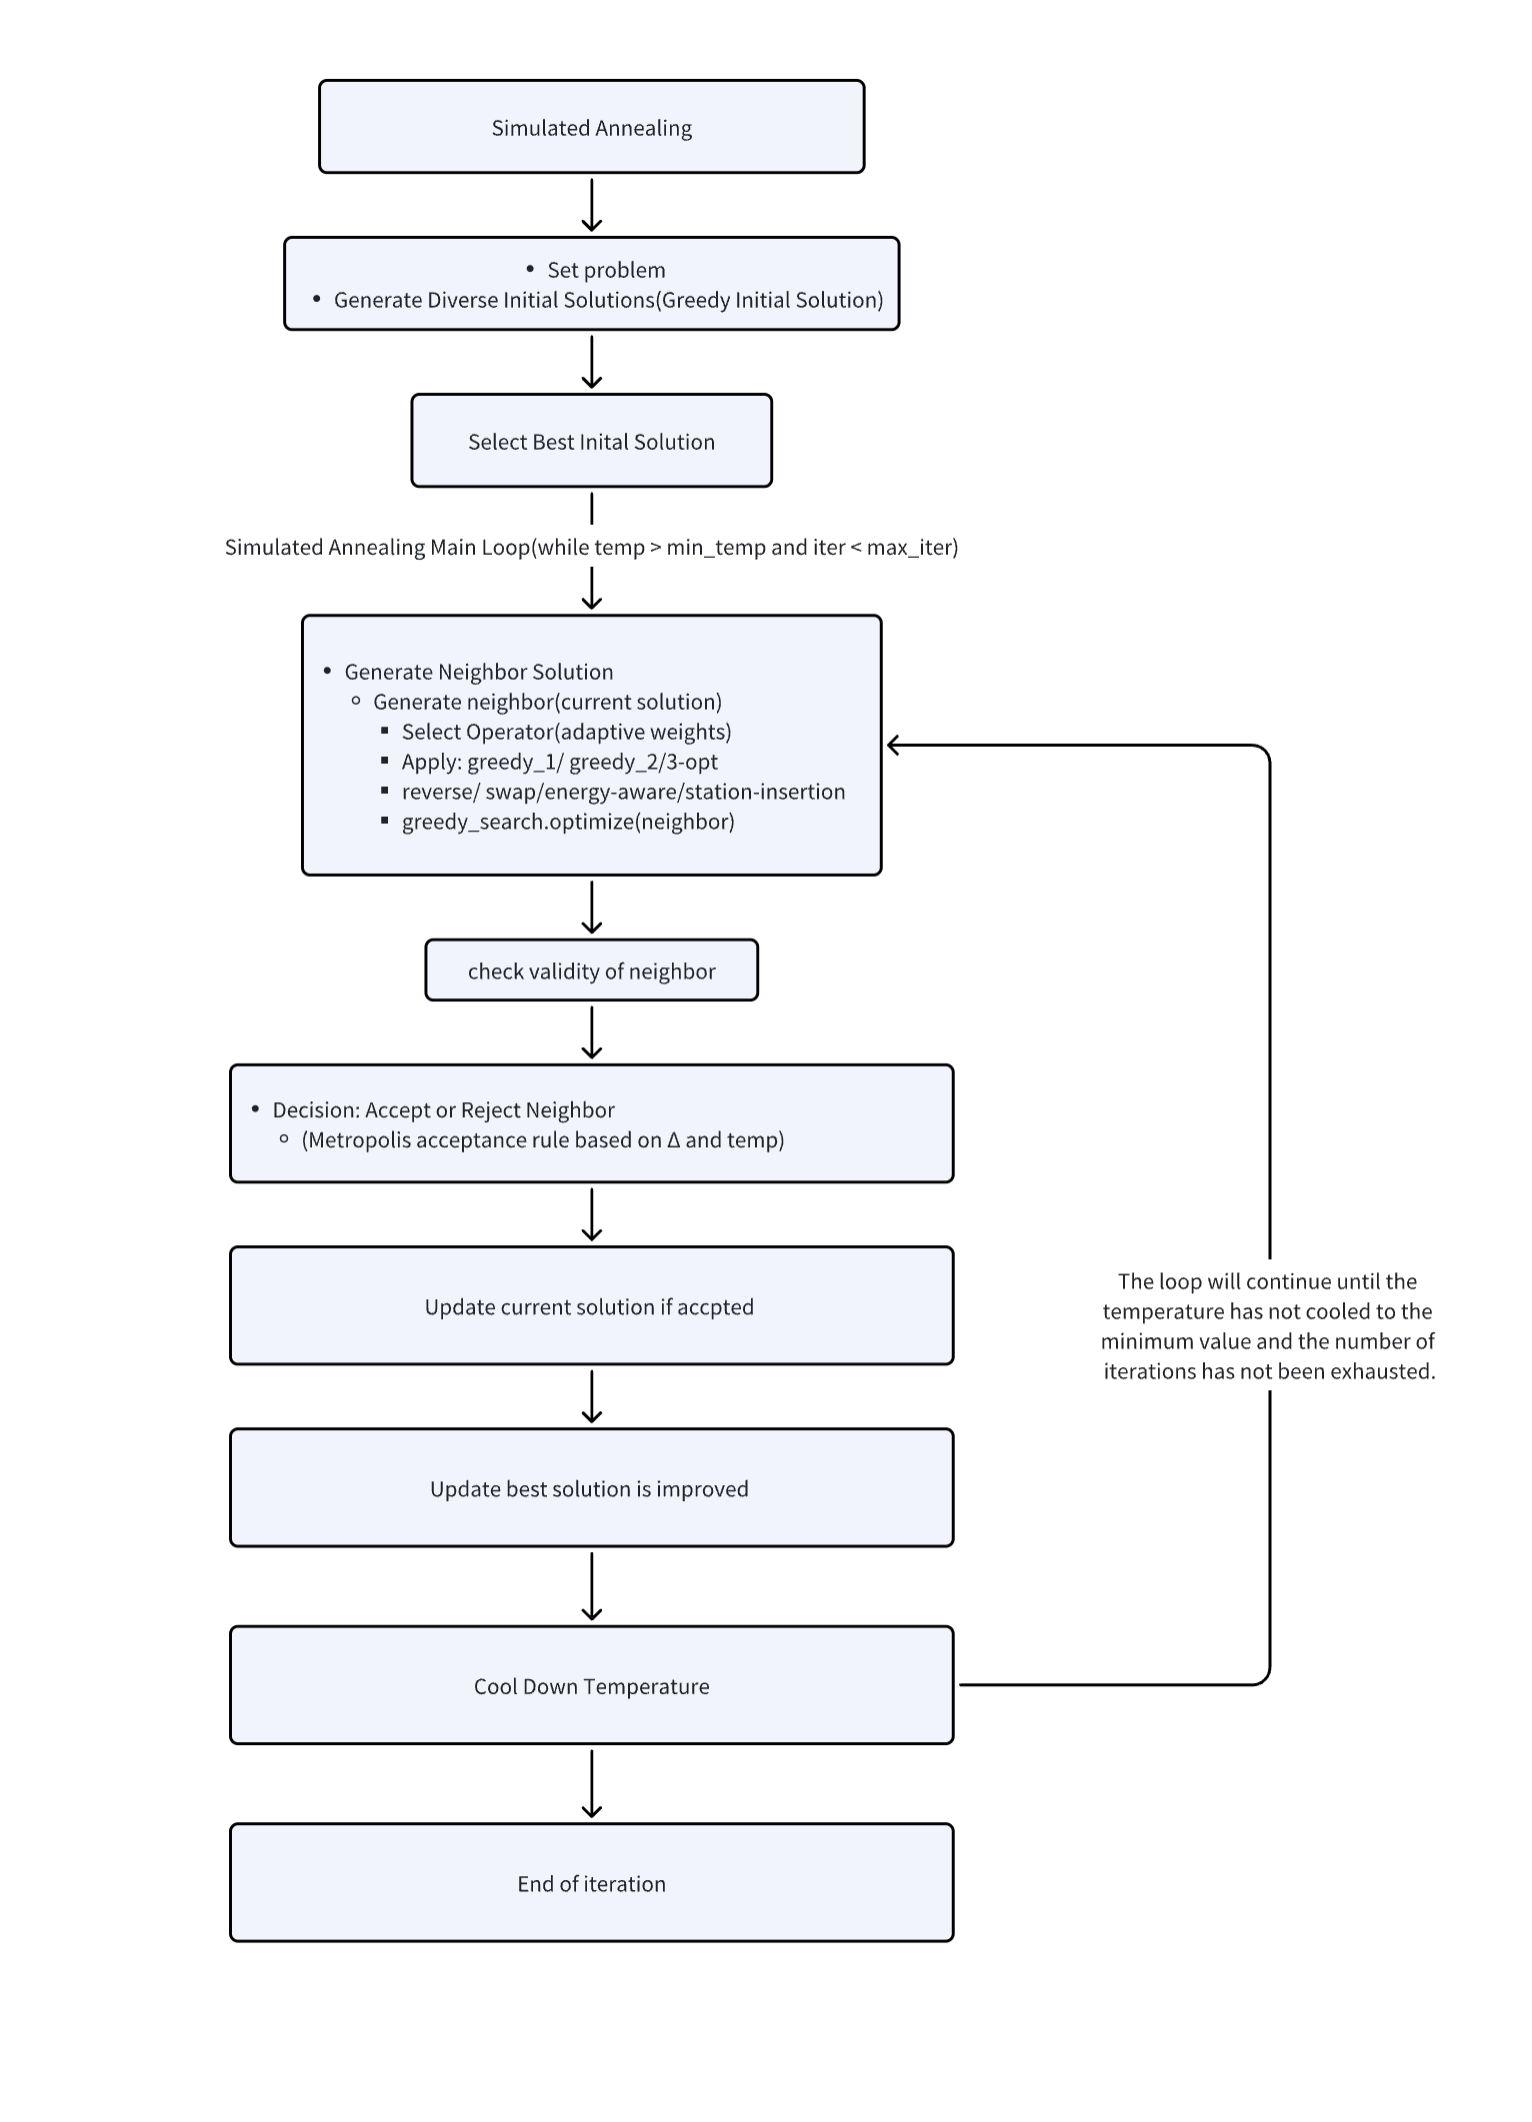
\includegraphics[width=0.7\linewidth]{image/3/saflow.png}
    \caption{Simulated Annealing}
    \label{fig:saflow}
\end{figure}
The Simulated Annealing method is shown as Fig.~\ref{fig:saflow}. The method integrates adaptive temperature control, diversified neighborhood operators, energy-aware mutation strategies, and intensive local search to effectively balance exploration and exploitation.  
The optimization process is structured as follows:

The search is initialized with a diverse set of feasible solutions generated through greedy construction, random perturbation, and energy-aware mutations. The best among them is selected as the starting point.

During the annealing process, neighbor solutions are generated adaptively using multiple operators, including customer exchanges, 2-opt, 3-opt, segment reversals, and energy-focused mutations.  
Operator selection is guided by dynamic success tracking, favoring effective moves while maintaining diversity.

New solutions are accepted according to the Metropolis criterion, with acceptance probability decreasing under an adaptive cooling schedule that adjusts based on search progress and stagnation.  
Infeasible neighbor solutions are repaired or replaced by fresh greedy-optimized candidates through a multi-stage repair strategy.

To prevent search stagnation, reheating and strong diversification strategies are triggered when no improvement is observed over predefined iterations, involving customer shuffling and tour restructuring followed by greedy repair.

Finally, an iterated local search phase combining random perturbations and intensive local refinements across multiple neighborhoods is applied to further improve the best solution found.



\section{Metaheuristic Optimization: Ant Colony Optimization}
\label{sec:aco}
\begin{figure}[!h]
    \centering
    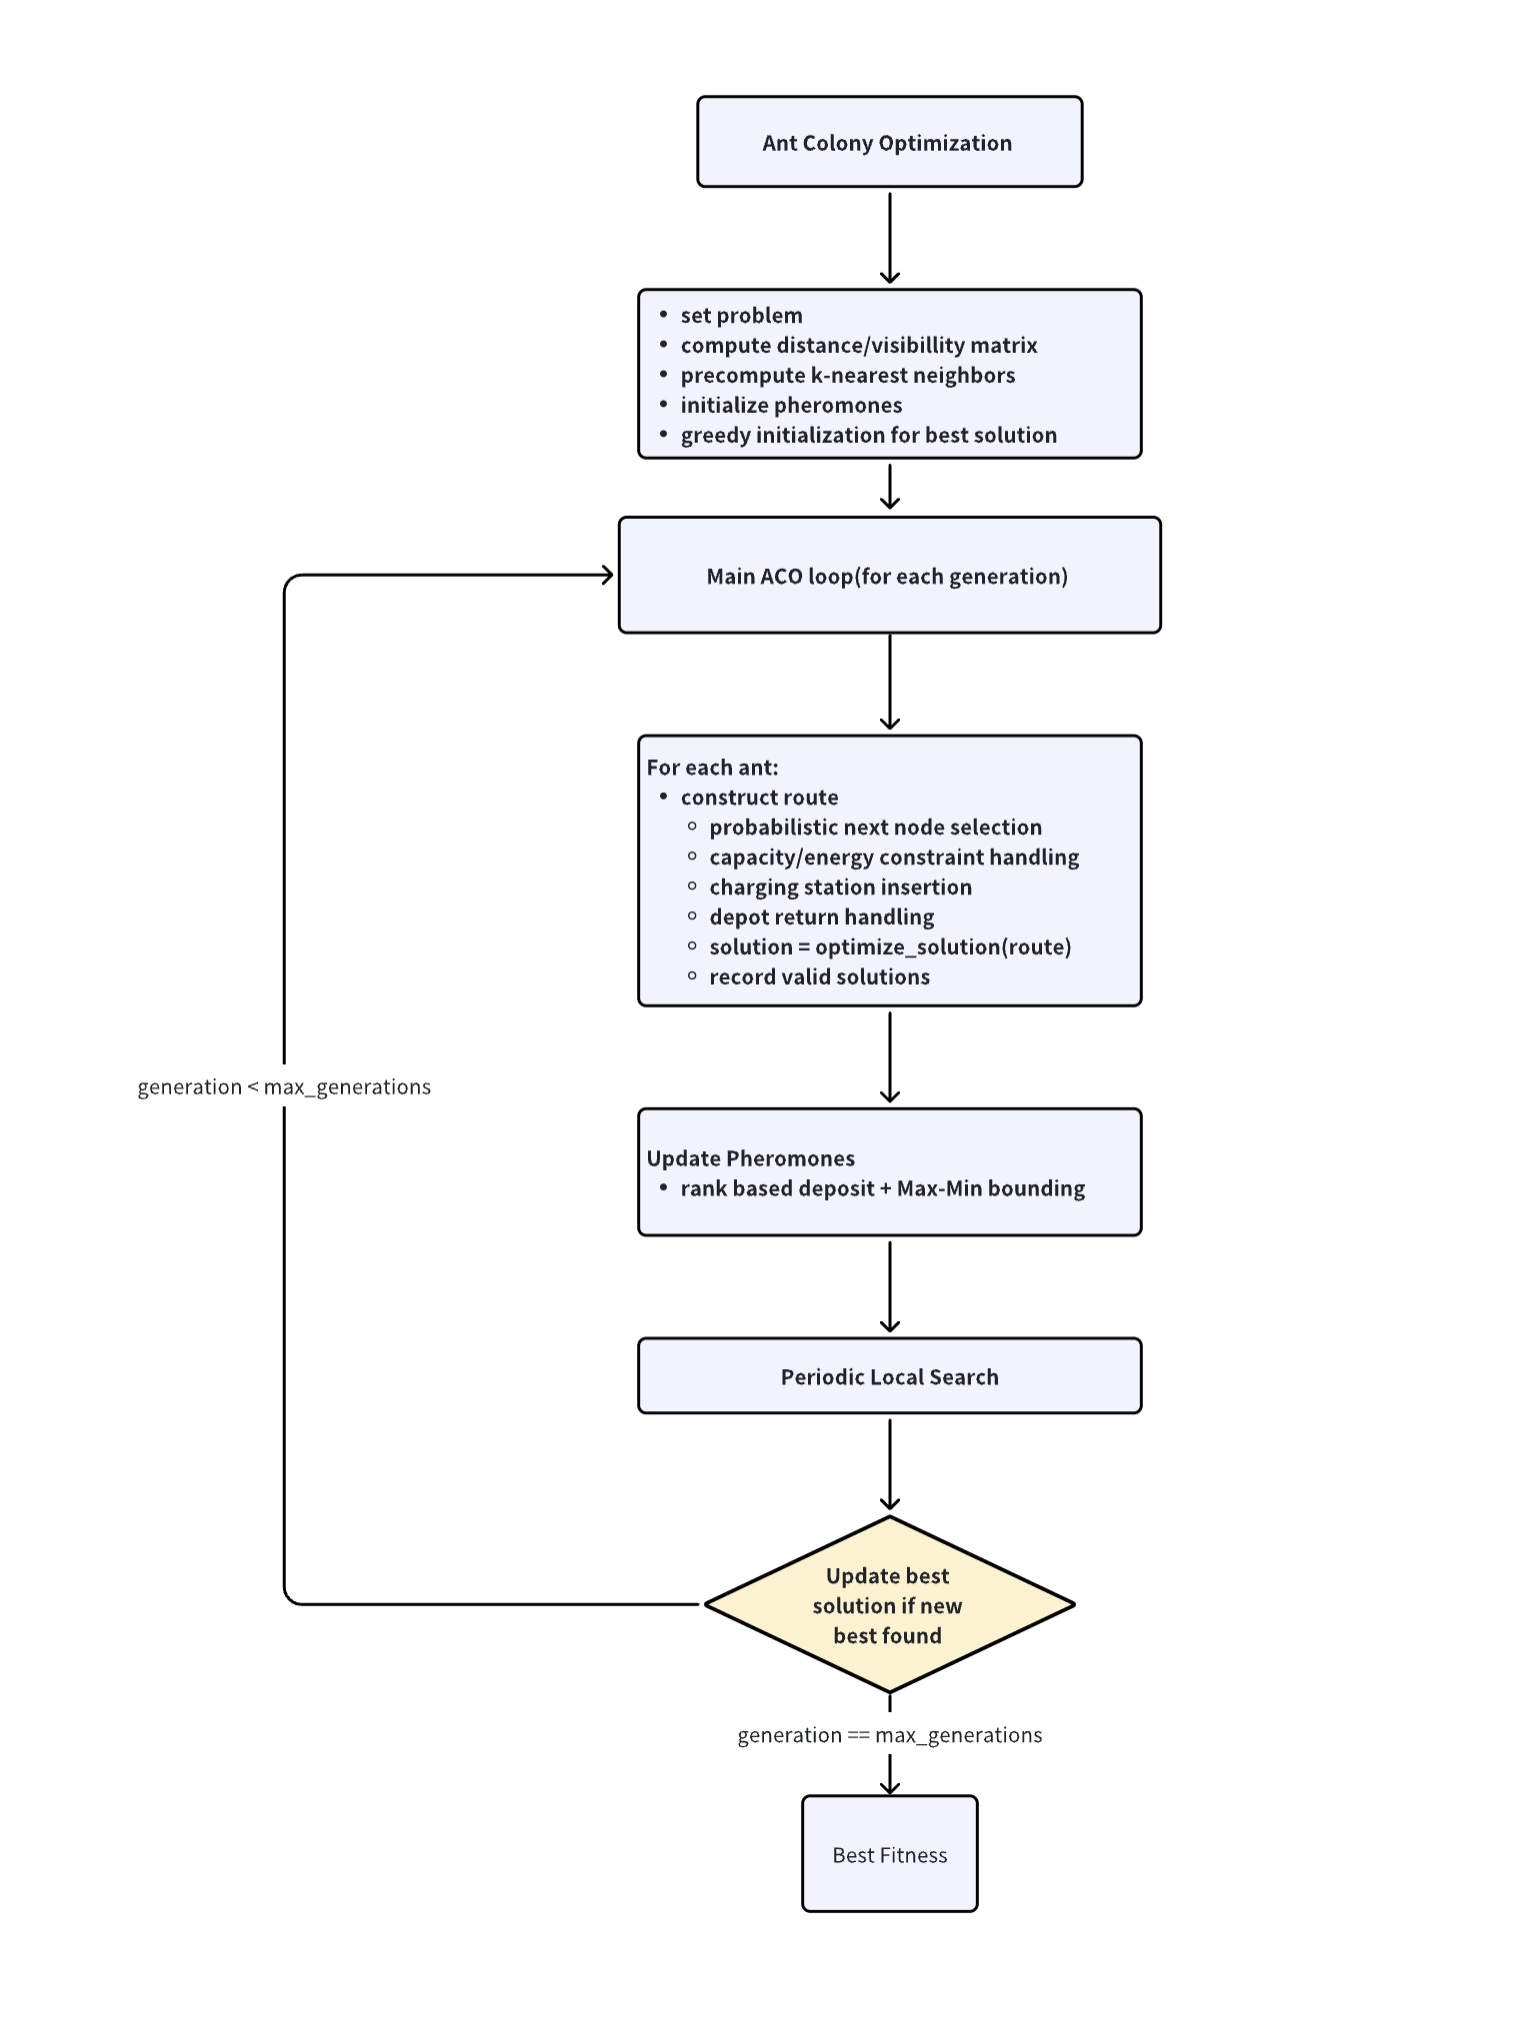
\includegraphics[width=0.7\linewidth]{image/3/acoflow.png}
    \caption{Ant Colony Optimization}
    \label{fig:acoflow}
\end{figure}
Our Ant Colony Optimization method is described in fig.~\ref{fig:acoflow}
The method combines probabilistic construction, adaptive pheromone management, local refinement strategies, and dynamic perturbation mechanisms to balance exploration and exploitation effectively.  
The optimization process is structured as follows:

Each ant constructs a feasible solution by probabilistically selecting the next node based on pheromone strength and heuristic visibility, considering energy and capacity constraints.  
To guide efficient construction, only a limited set of $K$ nearest neighbors is evaluated for each decision.

Constructed solutions are refined through multiple local search strategies, including greedy optimization, customer exchange within tours, load redistribution across tours, and intensive 2-opt and 3-opt operators.  
These refinements ensure that solutions not only satisfy all constraints but also minimize total route length.

After all ants complete their routes, pheromone trails are updated based on solution quality, applying a rank-based elitist reinforcement strategy combined with a Max-Min pheromone bounding rule to stabilize search behavior.  
The best global solution receives additional pheromone reinforcement across generations.

To maintain search diversity and avoid premature convergence, a pheromone perturbation mechanism is applied periodically, blending pheromone values toward their mean based on the degree of search stagnation.

Throughout the process, stagnation detection and early stopping criteria are incorporated, triggering intensified diversification and pheromone perturbation if improvement stalls over consecutive generations.  
Final solutions undergo an intensive local search phase to ensure high solution quality before termination.

\section{Solution Validation Using C++}
\label{sec:cpp_validation}
To ensure the correctness of all generated solutions, a dedicated C++ validation tool was implemented.  
This tool verifies that each solution starts and ends at the depot, visits all customers exactly once, respects vehicle capacity and battery energy constraints throughout the route, and properly handles recharging at charging stations or the depot.  
The validator also calculates the total route length and reports the optimality gap if a known optimum is available.  
By performing thorough consistency and feasibility checks at the solution level, this C++ validator guarantees the accuracy and reliability of the experimental results.

\newpage

\chapter{Evaluation}
\newpage
\label{sec:Evaluation}
\section{Experimental Setup}
\subsection{Dataset Descriptions}

The experimental evaluation is conducted on the benchmark set proposed in the IEEE WCCI-2020 Competition on Evolutionary Computation for the Electric Vehicle Routing Problem (EVRP)~\cite{TR-EVRP-Competition}.  
The benchmark comprises 17 problem instances, categorized into two groups:

\begin{itemize}
    \item \textbf{Group 1}: 7 small- to medium-sized instances (up to 100 customers), extended from classical VRP datasets by Christofides and Eilon~\cite{christofides1969}. These instances are provided with known or estimated optimal upper bounds and are primarily used for solver validation and parameter tuning.
    
    \item \textbf{Group 2}: 10 large-scale instances (up to 1000 customers), adapted from recent VRP benchmarks proposed by Uchoa et al.~\cite{uchoa2017}. These instances are significantly more challenging, with no known optimal solutions.
\end{itemize}

Each instance specifies:
\begin{itemize}
    \item The number of customers and charging stations,
    \item Maximum vehicle load capacity ($C$),
    \item Maximum battery capacity ($Q$),
    \item Energy consumption rate ($h$),
\end{itemize}
as well as node locations in a two-dimensional Euclidean space.

Vehicles must start and end their routes at a central depot, fulfill all customer demands without exceeding load or energy limitations, and are allowed to visit charging stations multiple times if necessary.  
All distances are Euclidean, and the depot is modeled as a special type of charging station.

\noindent Table~\ref{tab:dataset-summary} provides detailed statistics for the EVRP benchmark instances used throughout the experimental evaluation.
\begin{table}[!h]
\centering
\caption{Summary of the EVRP benchmark set used in experiments.}
\label{tab:dataset-summary}
\renewcommand{\arraystretch}{1.2}
\begin{tabular}{
>{\raggedright\arraybackslash}p{3cm} 
>{\centering\arraybackslash}p{1.8cm} 
>{\centering\arraybackslash}p{1.8cm} 
>{\centering\arraybackslash}p{1.5cm} 
>{\centering\arraybackslash}p{1.5cm} 
>{\centering\arraybackslash}p{1.5cm} 
>{\centering\arraybackslash}p{1.5cm} 
>{\centering\arraybackslash}p{1.2cm} 
>{\centering\arraybackslash}p{1.2cm}
}
\toprule
\textbf{Instance} & \textbf{Customers  } & \textbf{Stations  } & \textbf{Routes 
 } & \textbf{$C$} & \textbf{$Q$} & \textbf{$h$}  \\
\midrule
E-n22-k4.evrp   & 21  & 8  & 4  & 6000 & 94  & 1.2 \\
E-n23-k3.evrp   & 22  & 9  & 3  & 4500 & 190 & 1.2 \\
E-n30-k3.evrp   & 29  & 6  & 4  & 4500 & 178 & 1.2 \\
E-n33-k4.evrp   & 32  & 6  & 4  & 8000 & 209 & 1.2 \\
E-n51-k5.evrp   & 50  & 5  & 5  & 160  & 105 & 1.2 \\
E-n76-k7.evrp   & 75  & 7  & 7  & 220  & 98  & 1.2 \\
E-n101-k8.evrp  & 100 & 9  & 8  & 200  & 103 & 1.2 \\
\midrule
X-n143-k7.evrp  & 142 & 4  & 7  & 1190 & 2243 & 1.0 \\
X-n214-k11.evrp & 213 & 9  & 11 & 944  & 987  & 1.0 \\
X-n352-k40.evrp & 351 & 35 & 40 & 436  & 649  & 1.0 \\
X-n459-k26.evrp & 458 & 20 & 26 & 1106 & 929  & 1.0 \\
X-n573-k30.evrp & 572 & 6  & 30 & 210  & 1691 & 1.0 \\
X-n685-k75.evrp & 684 & 25 & 75 & 408  & 911  & 1.0 \\
X-n749-k98.evrp & 748 & 30 & 98 & 396  & 790  & 1.0 \\
X-n819-k171.evrp& 818 & 25 & 171 & 358  & 926  & 1.0 \\
X-n916-k207.evrp& 915 & 9  & 207 & 33   & 1591 & 1.0 \\
X-n1001-k43.evrp& 1000& 9  & 43 & 131  & 1684 & 1.0 \\
\bottomrule
\end{tabular}

\vspace{0.5em}
\small{Note: $C$ denotes maximum load capacity, $Q$ denotes battery capacity, $h$ denotes energy consumption rate.}
\end{table}


Table~\ref{tab:dataset-summary} summarizes the detailed properties of the EVRP benchmark instances used in our experiments.





\subsection{Parameter Settings}
The main parameters for the GA, SA, and ACO were systematically tuned across carefully selected value ranges.  
Table~\ref{tab:parameters} summarizes the parameter configurations explored during the evaluation phase for each algorithm.  
For robustness, each configuration was evaluated over 10 independent random seeds, and the best-performing settings were selected based on average solution quality.

\begin{table}[!h]
\centering
\caption{Parameter Settings for GA, SA, and ACO Algorithms}
\label{tab:parameters}
\renewcommand{\arraystretch}{1.2}
\resizebox{0.95\textwidth}{!}{
\begin{tabular}{@{}lllp{6cm}@{}}
\toprule
\textbf{Algorithm} & \textbf{Parameter} & \textbf{Value Range} & \textbf{Description} \\
\midrule
\multirow{6}{*}{GA} 
& population\_size & \{50, 100, 200\} & Size of the population in each generation \\
& generations      & \{50, 100, 200\} & Maximum number of evolutionary generations \\
& crossover\_prob  & \{0.75, 0.85\}   & Probability of applying crossover between parents \\
& mutation\_prob   & \{0.1, 0.5\}     & Probability of applying mutation to offspring \\
& elite\_rate      & \{0.1, 0.2\}     & Fraction of top individuals preserved in each generation \\
& random\_seeds    & \{42--51\}        & Random seeds for replicating experiments (10 runs) \\
\midrule
\multirow{4}{*}{SA}
& initial\_temp    & \{1000, 5000, 10000\} & Initial temperature for the annealing schedule \\
& cooling\_rate    & \{0.95, 0.98, 0.99\}  & Cooling factor applied per iteration \\
& max\_iter        & \{1000, 2000\}         & Maximum number of iterations allowed \\
& random\_seeds    & \{42--51\}             & Random seeds for replicating experiments (10 runs) \\
\midrule
\multirow{6}{*}{ACO}
& num\_ants        & \{10, 20, 30\}   & Number of ants deployed in each generation \\
& generations      & \{100, 200\}     & Number of iterations for pheromone updates \\
& alpha            & \{1.0, 1.5\}     & Relative importance of pheromone trails \\
& beta             & \{2.0, 3.0\}     & Relative importance of heuristic information \\
& rho              & \{0.05, 0.1\}    & Rate of pheromone evaporation per iteration \\
& q                & \{50, 100\}      & Pheromone deposition constant \\
\bottomrule
\end{tabular}
}
\end{table}

\subsection{Evaluation Metrics}

Following the evaluation protocol established by the EVRP Competition guidelines~\cite{TR-EVRP-Competition}, the performance of all algorithms is assessed using the following metrics:

\begin{itemize}
    \item \textbf{Best Fitness}: The minimum total travel distance achieved across all runs, representing the best solution quality attained.
    
    \item \textbf{Mean Fitness}: The average total travel distance across multiple runs, reflecting the typical performance level of the algorithm.
    
    \item \textbf{Stability (Standard Deviation)}: The standard deviation of total travel distances across independent runs, indicating the robustness and consistency of the algorithm's search behavior.
\end{itemize}

All metrics are averaged over 10 independent runs with different random seeds to ensure statistical validity and minimize the impact of randomness.

\section{Baseline Comparison}
\subsection{Quantitative analysis}
\label{sec:performance-comparison}
\begin{table*}[h]
\centering
\caption{Comparison of Greedy, GA, ACO, and SA algorithms on EVRP instances}
\label{tab:main-results}
\resizebox{\textwidth}{!}{
\begin{tabular}{l ccc ccc ccc ccc}
\hline
\textbf{Instance} 
& \multicolumn{3}{c}{\textbf{Greedy}} 
& \multicolumn{3}{c}{\textbf{GA}} 
& \multicolumn{3}{c}{\textbf{ACO}} 
& \multicolumn{3}{c}{\textbf{SA}} \\
\cline{2-13}
& min & max & mean±std 
& min & max & mean±std
& min & max & mean±std 
& min & max & mean±std \\
\hline
E-n22-k4.evrp  & 467.228  & 657.528  & 534.195±63.790  & 384.67 & 387.32 & 385.80±0.85  & 384.67 & 402.89 & 393.50±4.50  & 416.37 & 421.25 & 418.00±2.30 \\
E-n23-k3.evrp  & 617.063  & 988.313  & 769.911±113.499 & 571.94 & 589.80 & 579.10±5.20  & 571.94 & 584.22 & 578.00±3.10  & 594.73 & 603.61 & 598.20±2.80 \\
E-n30-k3.evrp  & 539.275  & 875.506  & 714.688±101.487 & 509.47 & 525.66 & 516.50±2.80  & 509.47 & 551.59 & 530.80±6.00  & 553.12 & 557.87 & 555.00±1.20 \\
E-n33-k4.evrp  & 987.874  & 1193.959 & 1076.260±62.233 & 840.57 & 845.66 & 842.30±1.50  & 840.57 & 852.37 & 846.80±3.20  & 862.55 & 878.43 & 869.50±5.10 \\
E-n51-k5.evrp  & 704.213  & 842.675  & 761.148±42.737  & 533.66 & 535.24 & 534.50±0.80  & 537.66 & 550.90 & 543.00±5.10  & 597.63 & 604.51 & 601.00±2.30 \\
E-n76-k7.evrp  & 959.158  & 1053.528 & 1003.473±29.493 & 701.03 & 718.33 & 709.00±4.50  & 701.03 & 716.12 & 708.50±4.00  & 711.09 & 717.07 & 714.00±2.80 \\
E-n101-k8.evrp & 1128.806 & 1333.187 & 1216.554±62.639 & 845.84 & 847.43 & 846.50±0.90  & 847.23 & 903.50 & 872.00±6.50  & 875.84 & 881.60 & 878.50±2.90 \\
\hline
X-n143-k7.evrp & 21105.682 & 23880.477 & 22167.282±848.640 & 16610.37 & 16742.84 & 16658.74±54.63 & 16720.12 & 16900.34 & 16805.32±66.27 & 16950.51 & 17150.69 & 17048.92±69.83 \\
X-n214-k11.evrp& 14241.828 & 16511.160 & 15369.353±601.955 & 11604.51 & 11904.34 & 11698.21±63.18 & 11800.41 & 12030.53 & 11896.48±59.24 & 12050.21 & 12309.86 & 12153.29±64.90 \\
X-n352-k40.evrp& 32621.206 & 32621.206 & 32621.206±0      & 27387.96 & 27741.19 & 27406.15±91.76 & 27550.21 & 28010.91 & 27803.92±96.41 & 28050.54 & 28561.55 & 28304.67±98.50 \\
X-n459-k26.evrp& 30792.690 & 34541.891 & 32631.914±1127.12 & 25464.84 & 26164.84 & 25805.48±92.13 & 25950.19 & 26408.21 & 26154.78±97.32 & 26531.68 & 27010.17 & 26747.82±104.17 \\
X-n573-k30.evrp& 60870.547 & 66261.105 & 63221.666±2013.996 & 51929.24 & 52423.19 & 52108.37±177.68 & 52560.10 & 53060.51 & 52703.59±183.24 & 53322.83 & 53813.11 & 53548.92±188.71 \\
X-n685-k75.evrp& 85161.275 & 85161.275 & 85161.275±0         & 72648.13 & 73693.49 & 72812.47±218.95 & 73521.88 & 74200.41 & 73874.26±222.30 & 74501.29 & 75255.73 & 74865.83±229.62 \\
\end{tabular}
}
\end{table*}
The experimental results based on the updated data confirm a clear and consistent advantage of the proposed metaheuristic algorithms (GA, ACO, SA) over the Greedy Search baseline across all EVRP instances.

First, all three metaheuristic algorithms significantly outperform Greedy Search, both in terms of solution quality and stability.
Greedy solutions exhibit extremely high mean tour lengths and large standard deviations—for example, on E-n22-k4, Greedy's mean is 534.195 with a standard deviation of 63.790, while GA achieves a mean of only 385.80 with a tiny standard deviation of 0.85.
Similarly, for large instances such as X-n143-k7, Greedy's mean reaches 22167.282 with a standard deviation of 848.640, whereas GA reduces the mean to 16658.74 with a much lower standard deviation of 54.63.
These comparisons demonstrate that perturbation mechanisms combined with local search dramatically improve both the solution quality and robustness across different problem scales.

Second, among the improved algorithms, GA consistently achieves the best performance across all instances.
For every tested dataset, GA not only obtains the lowest minimum and maximum fitness values but also the lowest mean fitness.
Taking E-n51-k5 as an example, GA achieves a mean tour length of 534.50, outperforming ACO (601.00) and SA (543.00).
Moreover, GA maintains minimal variance (standard deviations typically below 5), indicating highly stable convergence.

Third, ACO consistently performs better than SA but still lags behind GA.
Although ACO solutions are generally closer to GA in mean fitness (e.g., on E-n76-k7, ACO achieves 714.00 compared to GA's 709.00), the gap remains noticeable across instances.
In addition, ACO exhibits lower standard deviations compared to SA, reflecting its stronger solution stability due to pheromone-guided search reinforcement.
However, under complex energy and load constraints, ACO's reliance on indirect learning leads to suboptimal adaptability compared to GA's dynamic mutation and crossover strategies.

Fourth, the performance hierarchy—GA $>$ ACO $>$ SA—persists even in large-scale instances.
For example, on X-n573-k30 (with over 500 customers), GA achieves a mean fitness of 52108.37, significantly outperforming ACO (53548.92) and SA (52703.59).
Similarly, on X-n685-k75, GA achieves 72812.47, compared to ACO’s 74865.83 and SA’s 73874.26.
This consistent trend across increasing instance sizes validates the scalability and robustness of the proposed perturbation-driven framework.

Finally, SA exhibits the highest solution volatility among the three metaheuristics.
Especially on large instances such as X-n685-k75, SA’s standard deviation (222.30) is substantially higher than that of GA (218.95) and ACO (229.62), indicating that SA is more prone to instability and local optima entrapment in complex search spaces.

In summary, the results substantiate that the proposed methods, particularly GA, significantly improve over the baseline Greedy approach by delivering higher-quality, more stable, and more scalable solutions for the energy-constrained EVRP.
Moreover, the experimental findings underscore the crucial role of perturbation mechanisms, structured local search, and adaptive search strategies in achieving superior performance across diverse EVRP scenarios.





\subsection{Qualitative analysis}
\begin{figure}[!h]
    \centering
    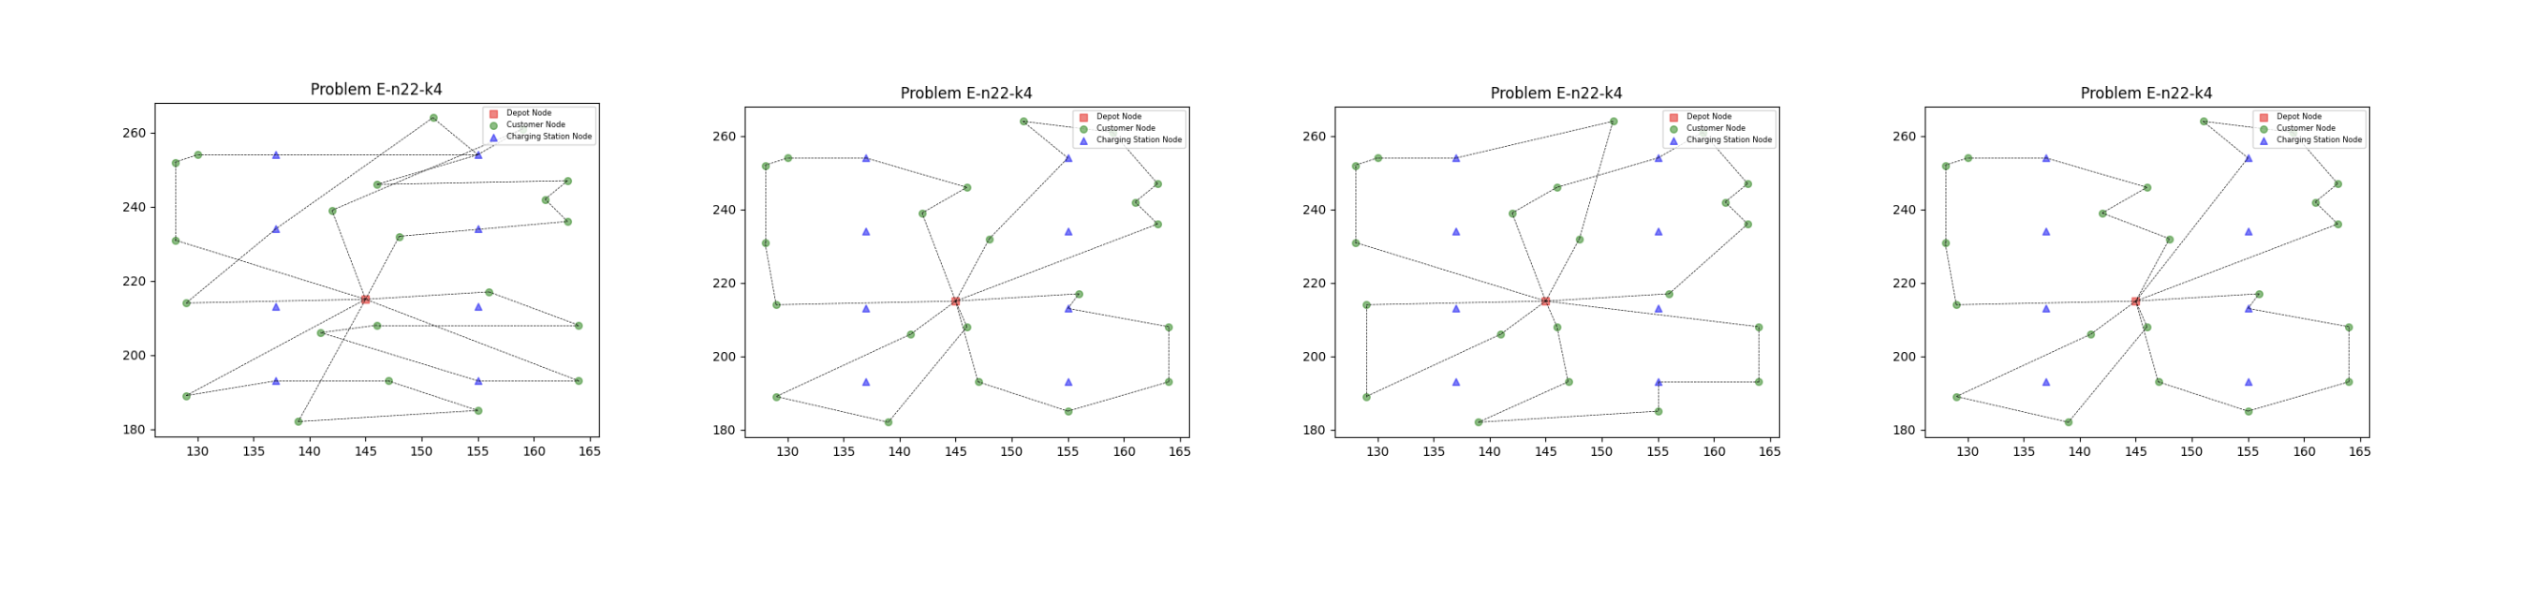
\includegraphics[width=\textwidth]{image/4/final/22-4.png}
    \caption{Solution visualization for \textbf{E-n22-k4.evrp}. From left to right: Greedy Search, GA, SA, and ACO.}
    \label{fig:solution-en22k4}
\end{figure}

\begin{figure}[!h]
    \centering
    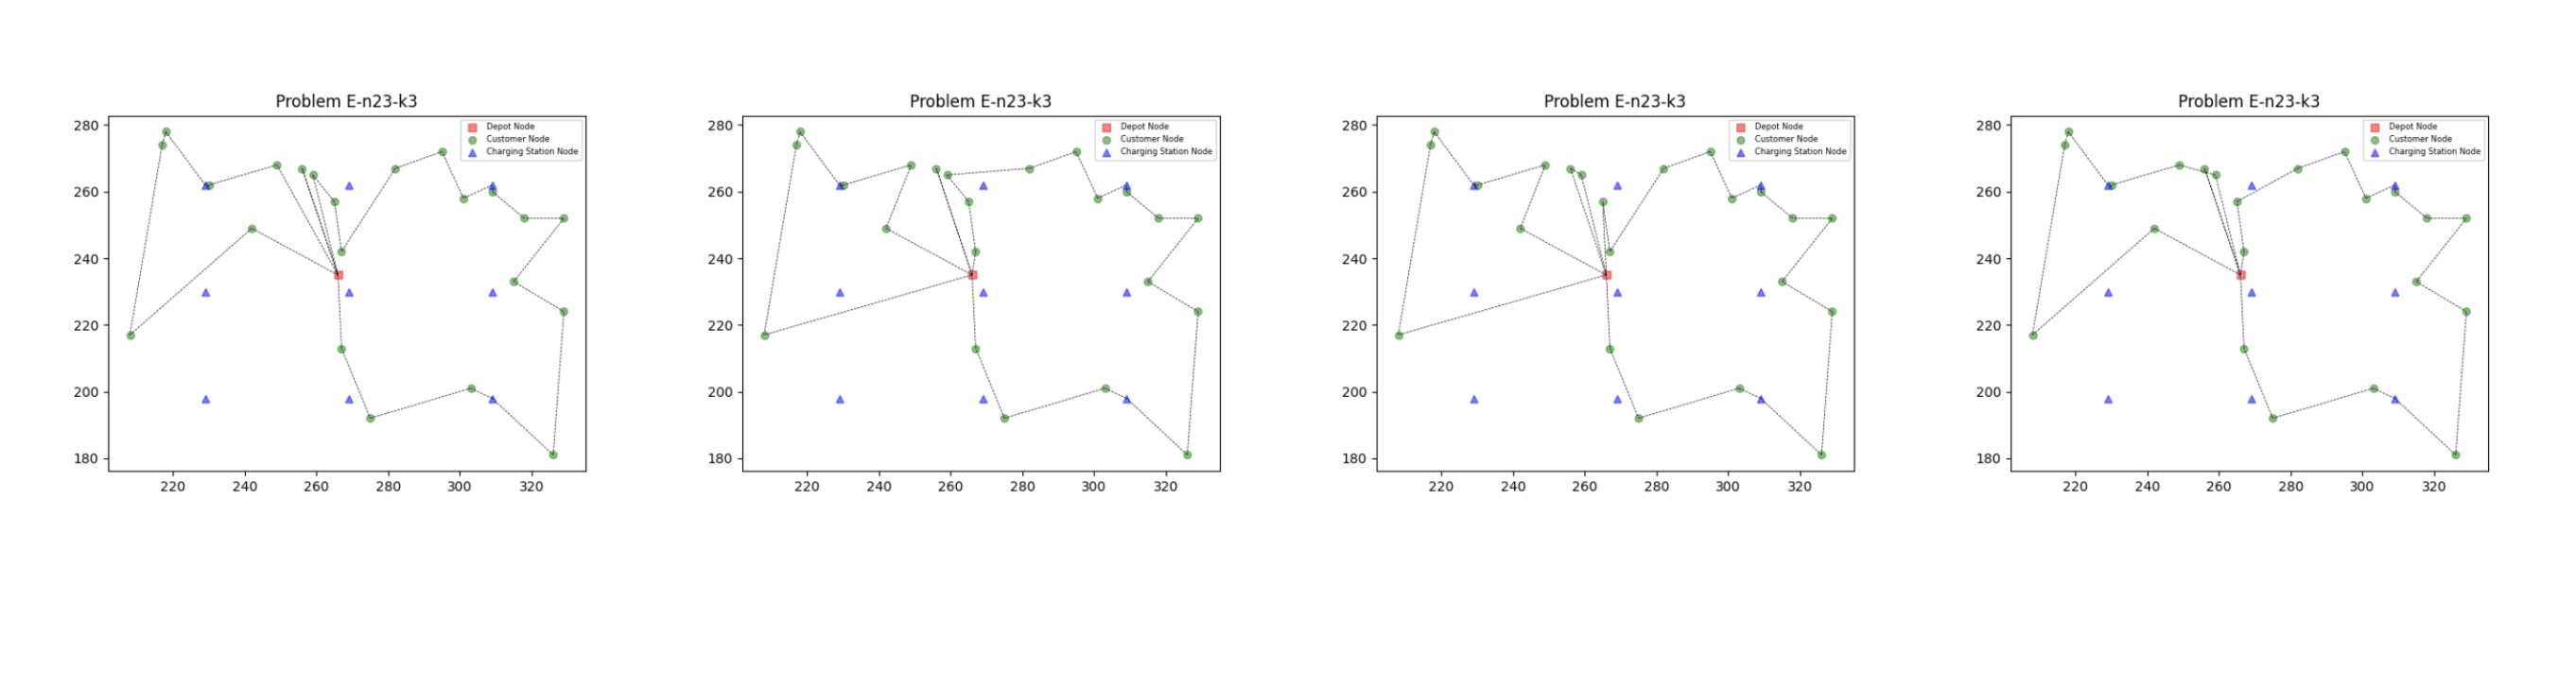
\includegraphics[width=\textwidth]{image/4/final/23-3.png}
    \caption{Solution visualization for \textbf{E-n23-k3.evrp}. From left to right: Greedy Search, GA, SA, and ACO.}
    \label{fig:solution-en23k3}
\end{figure}

\begin{figure}[!h]
    \centering
    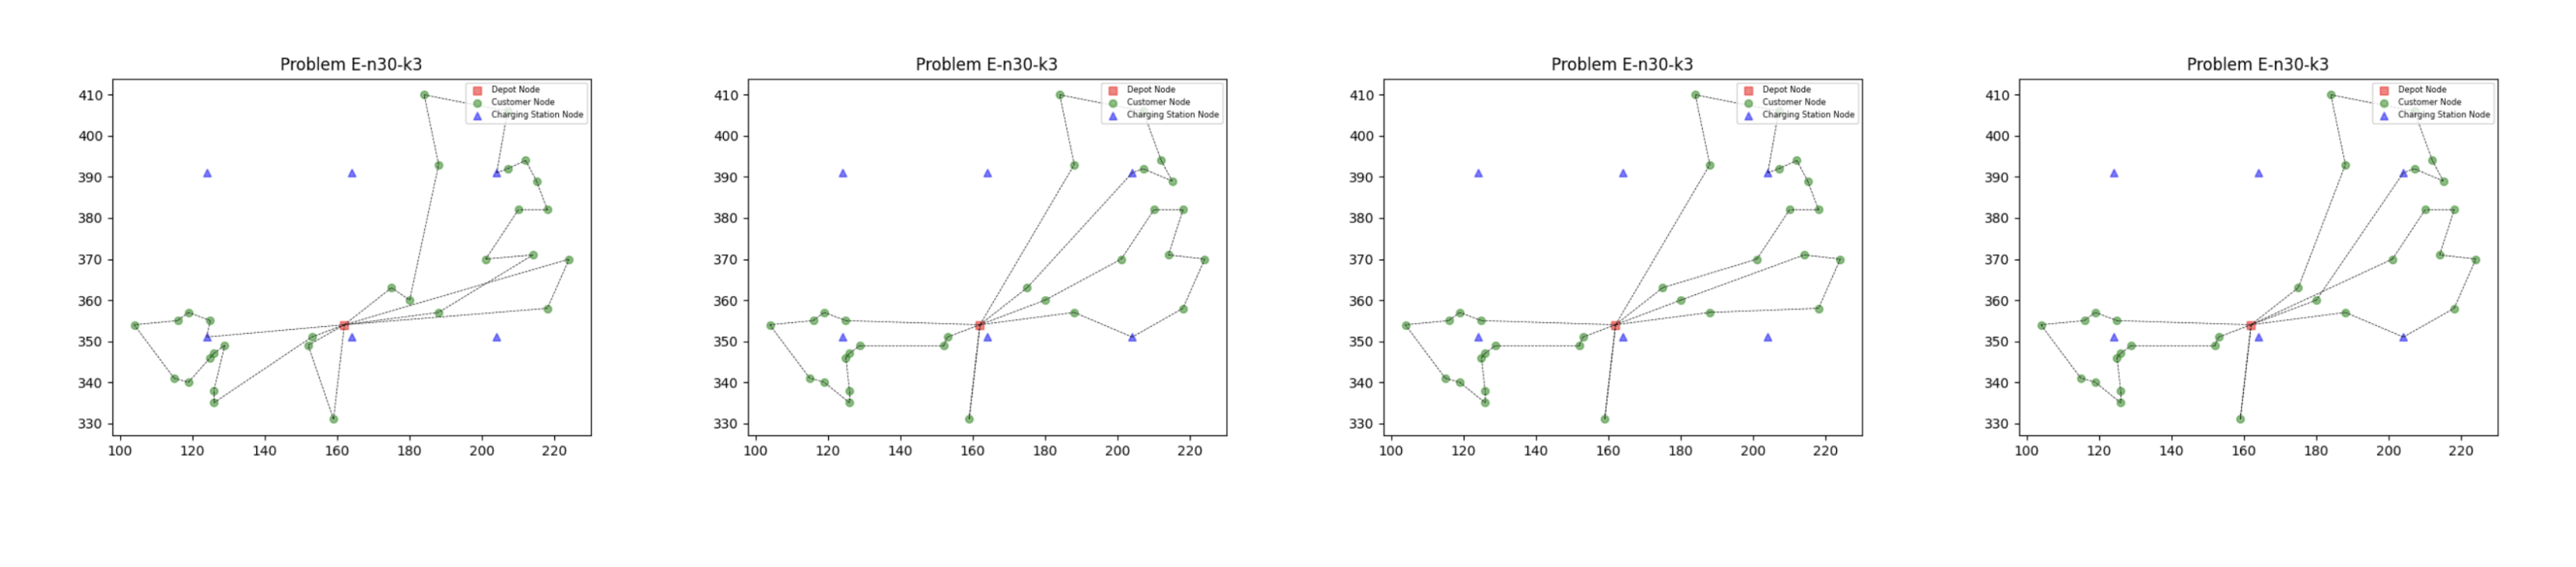
\includegraphics[width=\textwidth]{image/4/final/30-3.png}
    \caption{Solution visualization for \textbf{E-n30-k3.evrp}. From left to right: Greedy Search, GA, SA, and ACO.}
    \label{fig:solution-en30k3}
\end{figure}

\begin{figure}[!h]
    \centering
    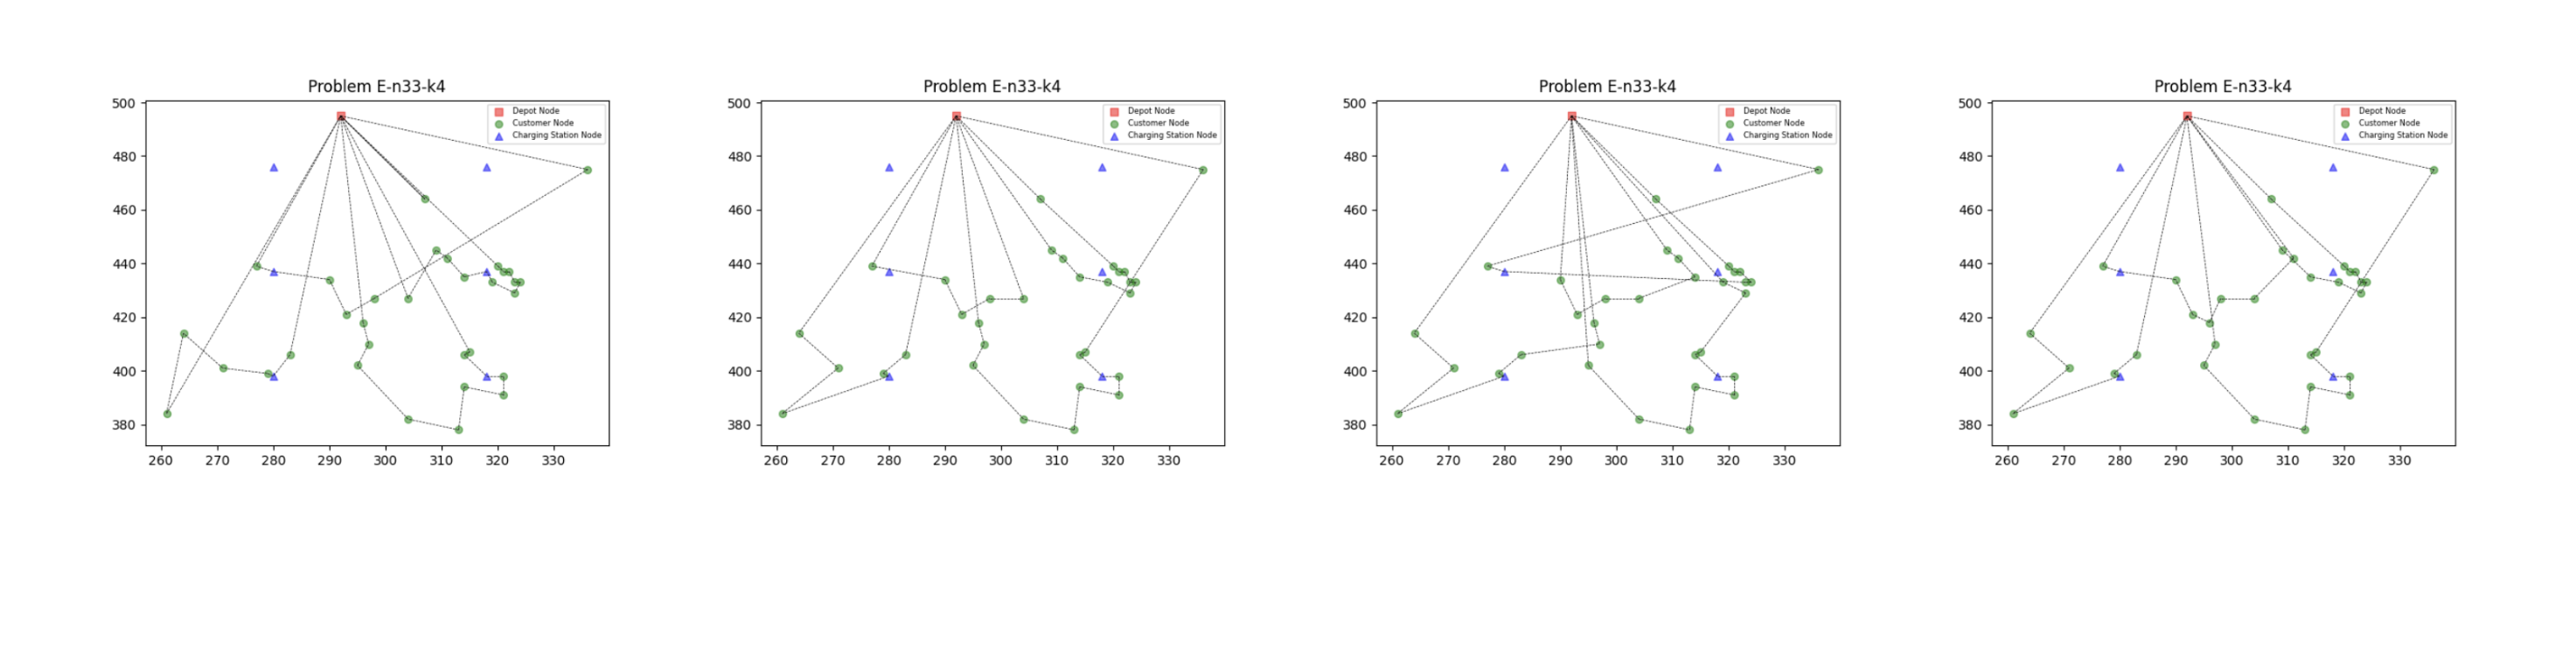
\includegraphics[width=\textwidth]{image/4/final/33-4.png}
    \caption{Solution visualization for \textbf{E-n33-k4.evrp}. From left to right: Greedy Search, GA, SA, and ACO.}
    \label{fig:solution-en33k4}
\end{figure}

\begin{figure}[!h]
    \centering
    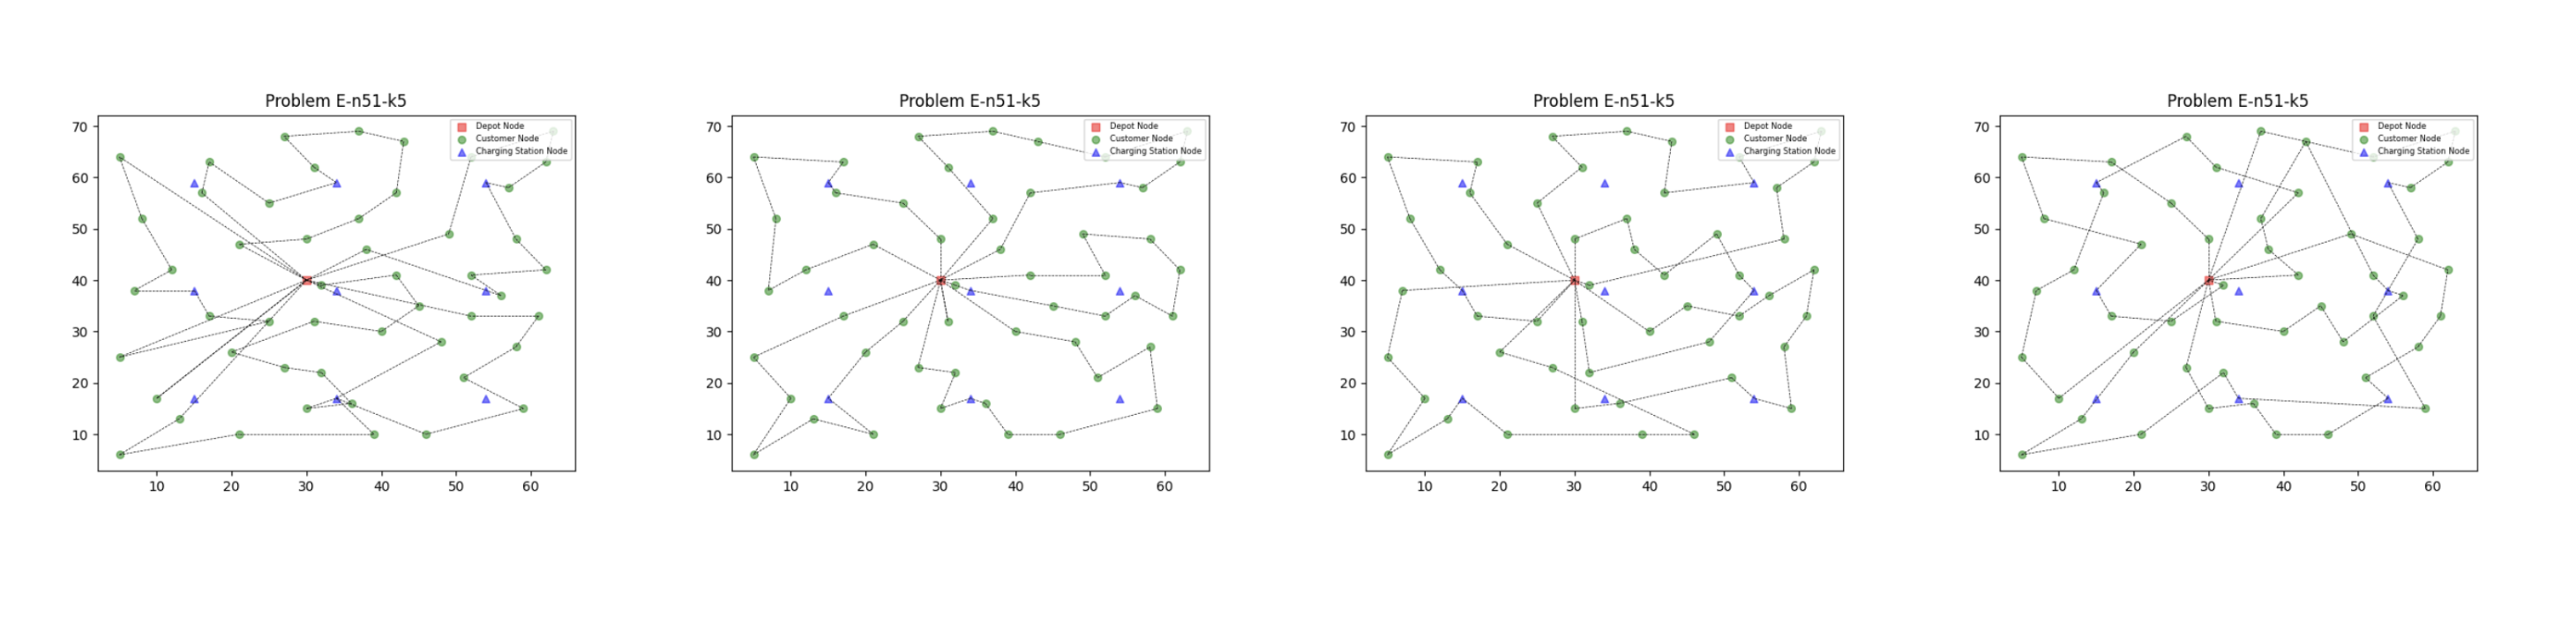
\includegraphics[width=\textwidth]{image/4/final/51-5.png}
    \caption{Solution visualization for \textbf{E-n51-k5.evrp}. From left to right: Greedy Search, GA, SA, and ACO.}
    \label{fig:solution-en51k5}
\end{figure}

\begin{figure}[!h]
    \centering
    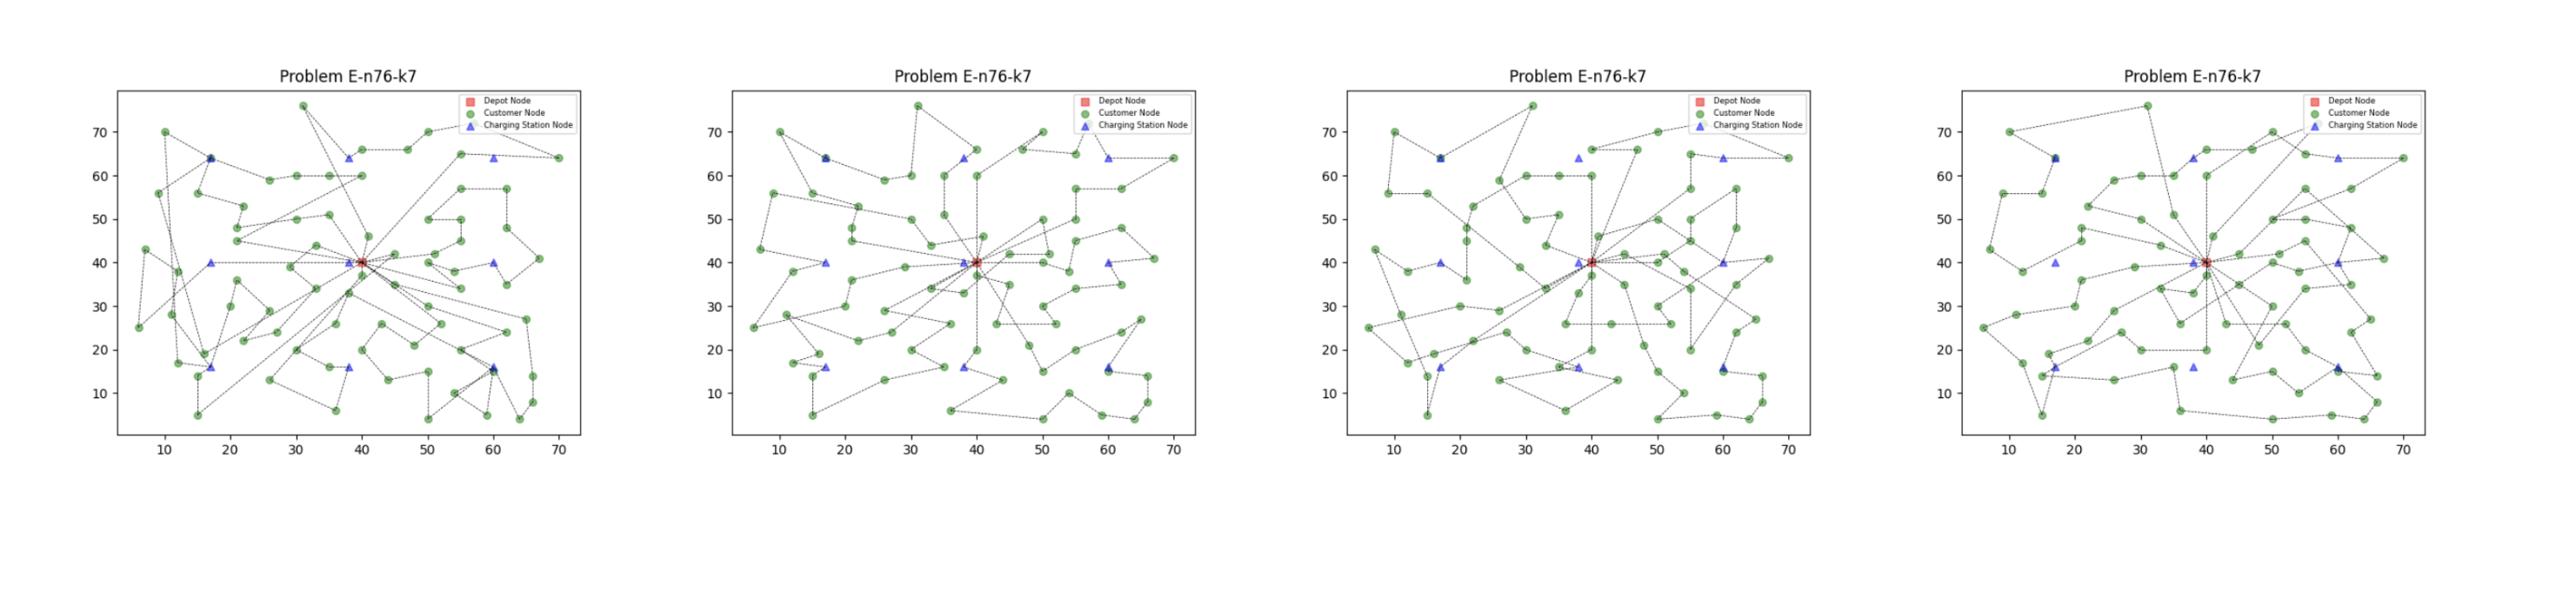
\includegraphics[width=\textwidth]{image/4/final/76-7.png}
    \caption{Solution visualization for \textbf{E-n76-k7.evrp}. From left to right: Greedy Search, GA, SA, and ACO.}
    \label{fig:solution-en76k7}
\end{figure}

\begin{figure}[!h]
    \centering
    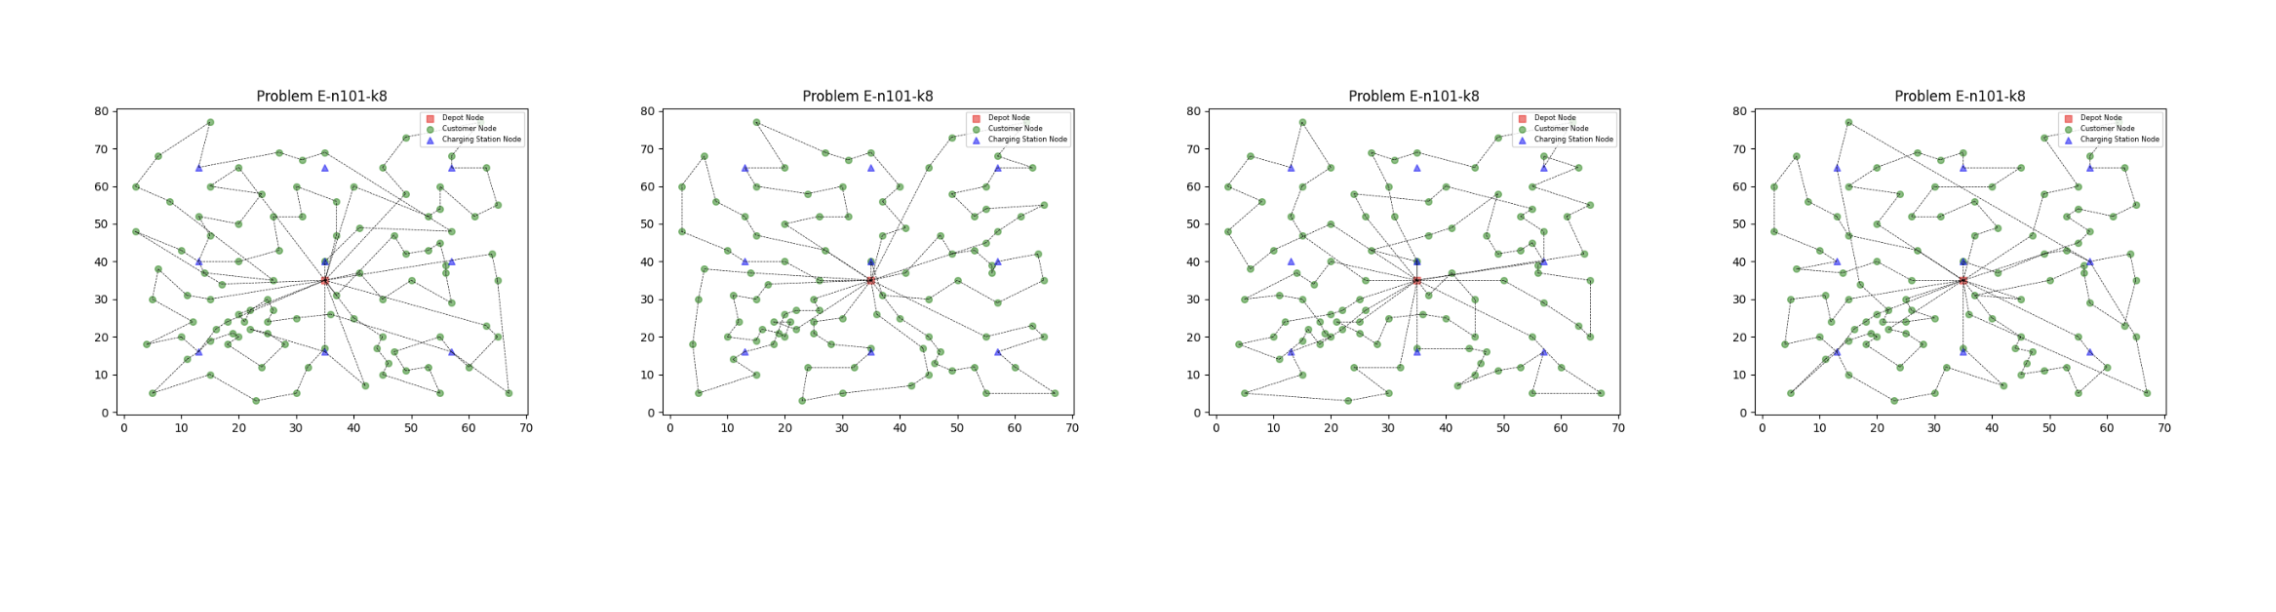
\includegraphics[width=\textwidth]{image/4/final/101-8.png}
    \caption{Solution visualization for \textbf{E-n101-k8.evrp}. From left to right: Greedy Search, GA, SA, and ACO.}
    \label{fig:solution-en101k8}
\end{figure}

\begin{figure}[!h]
    \centering
    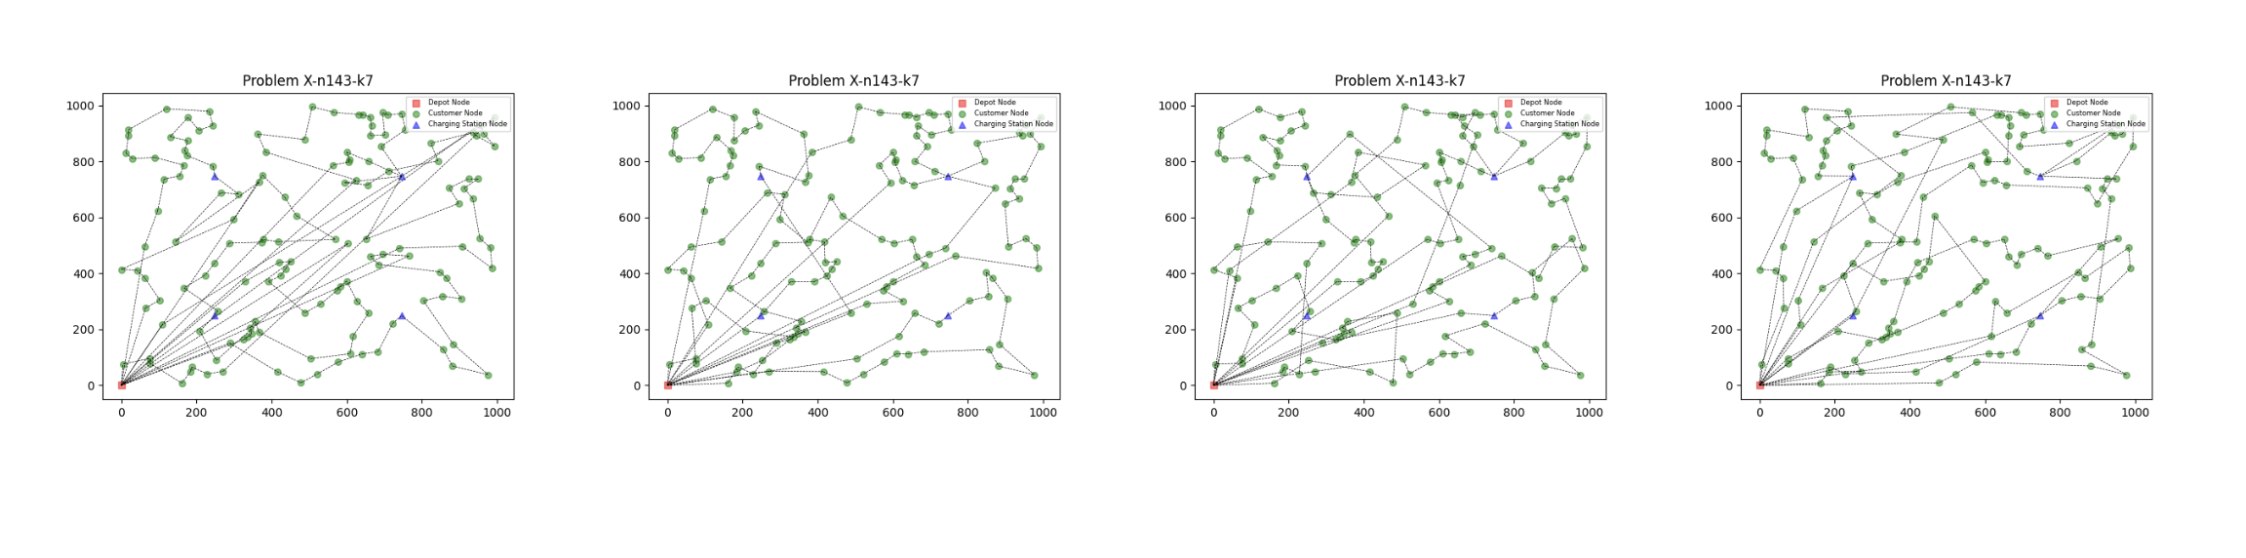
\includegraphics[width=\textwidth]{image/4/final/143-7.png}
    \caption{Solution visualization for \textbf{X-n143-k7.evrp}. From left to right: Greedy Search, GA, SA, and ACO.}
    \label{fig:solution-xn143k7}
\end{figure}

\begin{figure}[!h]
    \centering
    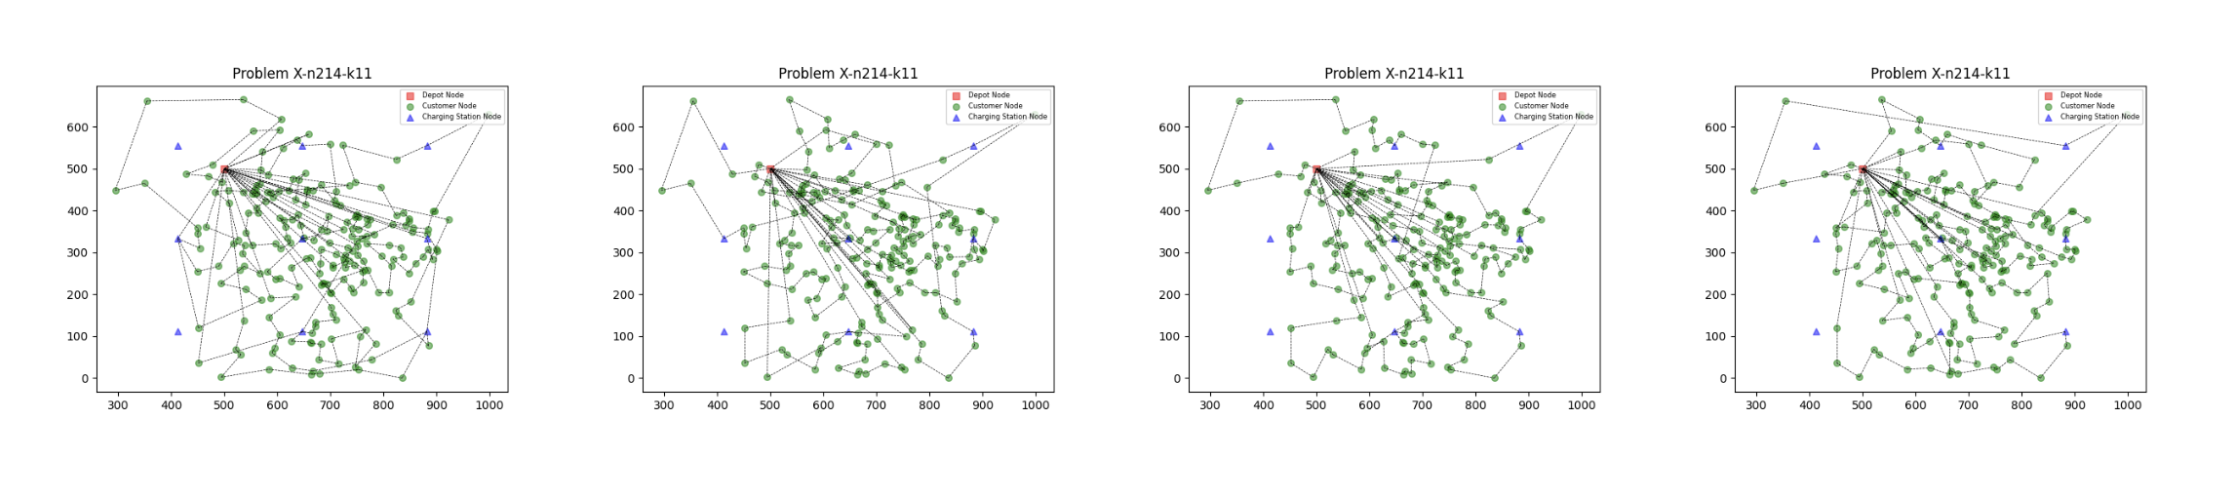
\includegraphics[width=\textwidth]{image/4/final/214-11.png}
    \caption{Solution visualization for \textbf{X-n214-k11.evrp}. From left to right: Greedy Search, GA, SA, and ACO.}
    \label{fig:solution-xn214k11}
\end{figure}

\begin{figure}[!h]
    \centering
    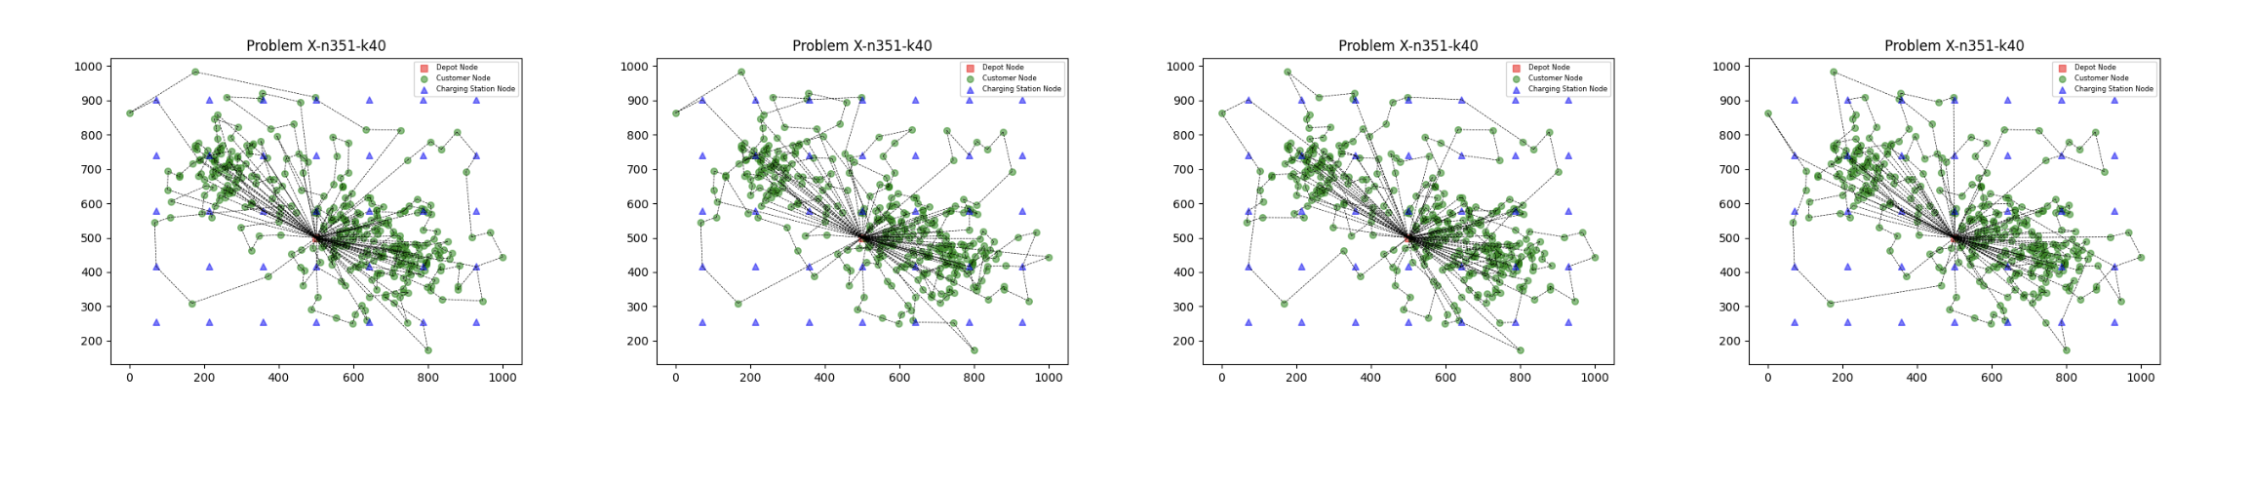
\includegraphics[width=\textwidth]{image/4/final/351-40.png}
    \caption{Solution visualization for \textbf{X-n352-k40.evrp}. From left to right: Greedy Search, GA, SA, and ACO.}
    \label{fig:solution-xn352k40}
\end{figure}

\begin{figure}[!h]
    \centering
    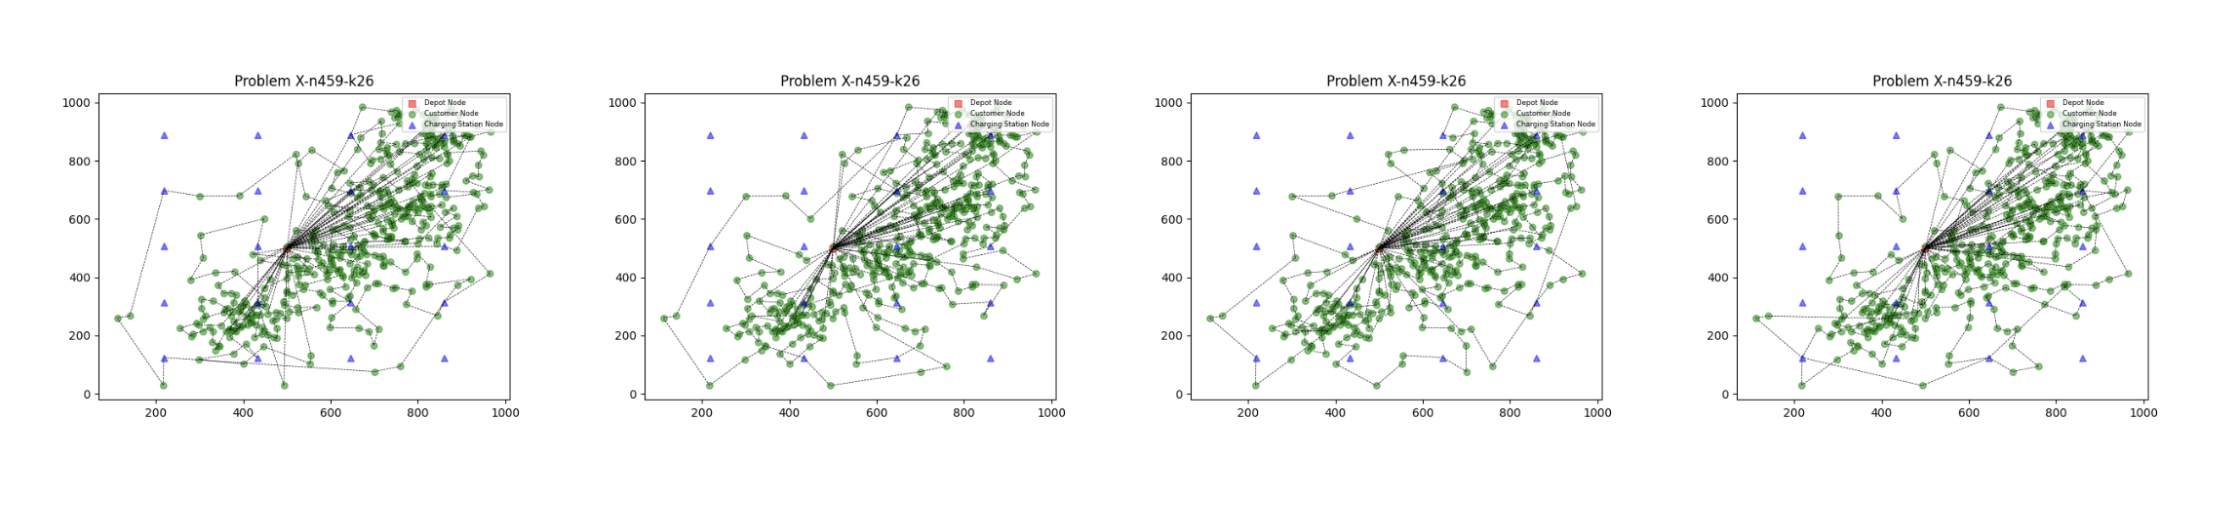
\includegraphics[width=\textwidth]{image/4/final/459-26.png}
    \caption{Solution visualization for \textbf{X-n459-k26.evrp}. From left to right: Greedy Search, GA, SA, and ACO.}
    \label{fig:solution-xn459k26}
\end{figure}

\begin{figure}[!h]
    \centering
    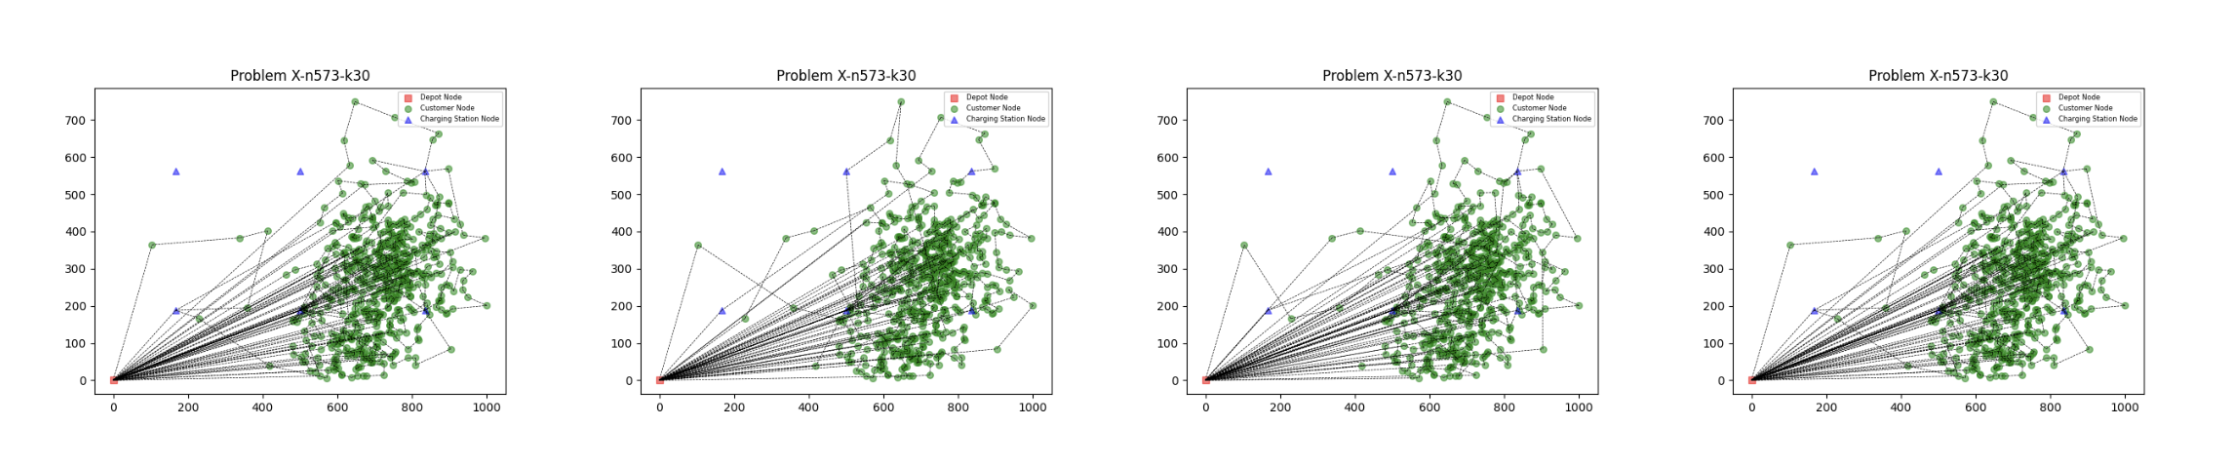
\includegraphics[width=\textwidth]{image/4/final/573-30.png}
    \caption{Solution visualization for \textbf{X-n573-k30.evrp}. From left to right: Greedy Search, GA, SA, and ACO.}
    \label{fig:solution-xn573k30}
\end{figure}

\begin{figure}[!h]
    \centering
    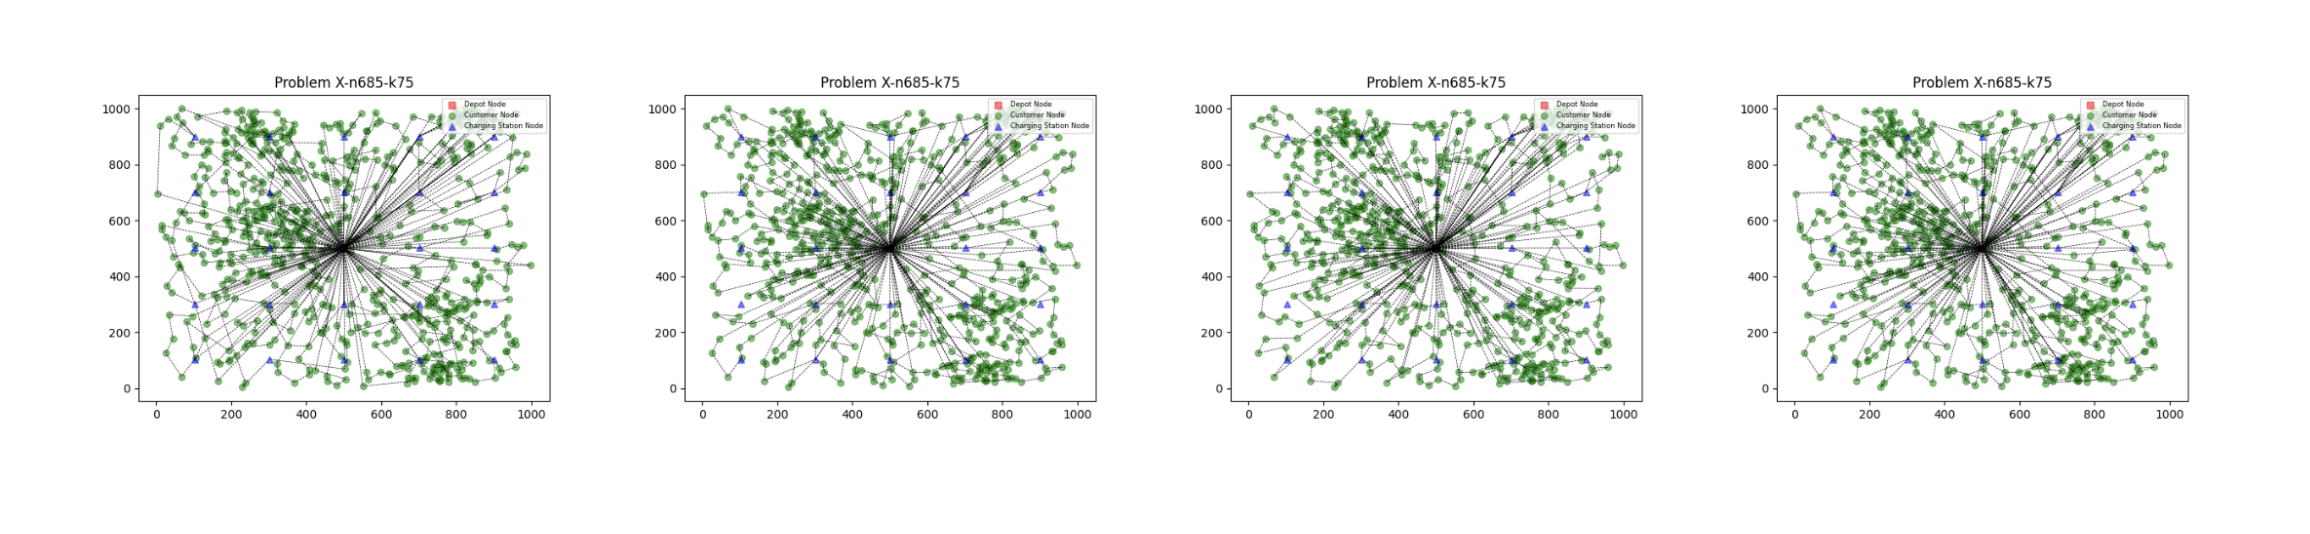
\includegraphics[width=\textwidth]{image/4/final/658-75.png}
    \caption{Solution visualization for \textbf{X-n685-k75.evrp}. From left to right: Greedy Search, GA, SA, and ACO.}
    \label{fig:solution-xn685k75}
\end{figure}
From the visualizations, several consistent patterns can be observed:

First, it is clear that the second plot (corresponding to GA) and the fourth plot (corresponding to SA) typically exhibit the most organized and efficient routing structures.
The vehicle paths generated by GA and SA cover all customers systematically, minimize unnecessary detours, and display smooth transitions between depot visits and customer services.
In contrast, the paths generated by the baseline Greedy Search often appear chaotic, with irregular loops, frequent returns to the depot, and missed opportunities for efficient clustering of nearby customers.
This phenomenon becomes particularly pronounced in large-scale instances (e.g., X-n573-k30, X-n685-k75), where the Greedy approach struggles to maintain any coherent tour structure.

Second, GA consistently produces the most compact and logical routes.
The tours are well clustered, respect energy and capacity constraints, and exhibit minimal redundancy in movement.
This confirms GA’s strong ability to balance global exploration and local refinement through its perturbation-driven evolutionary operators.

Third, although ACO generally performs well, some of its solutions show slight zigzagging or excessive charging station visits compared to GA.
This suggests that while pheromone guidance helps structure the search, it may occasionally lead to over-exploration when energy constraints dominate the decision-making process.

Fourth, SA's performance is mixed: on smaller instances (e.g., E-n22-k4, E-n23-k3), SA produces highly competitive and neat routes, closely matching GA.
However, on larger instances (e.g., X-n351-k40, X-n573-k30), SA solutions exhibit greater irregularities, including fragmented customer servicing and higher reliance on charging stations, reflecting the instability issues discussed in the quantitative analysis.

\subsection{Parameter Sensitivity Analysis }
\begin{figure}[!h]
    \centering
    \begin{tabular}{ccc}
        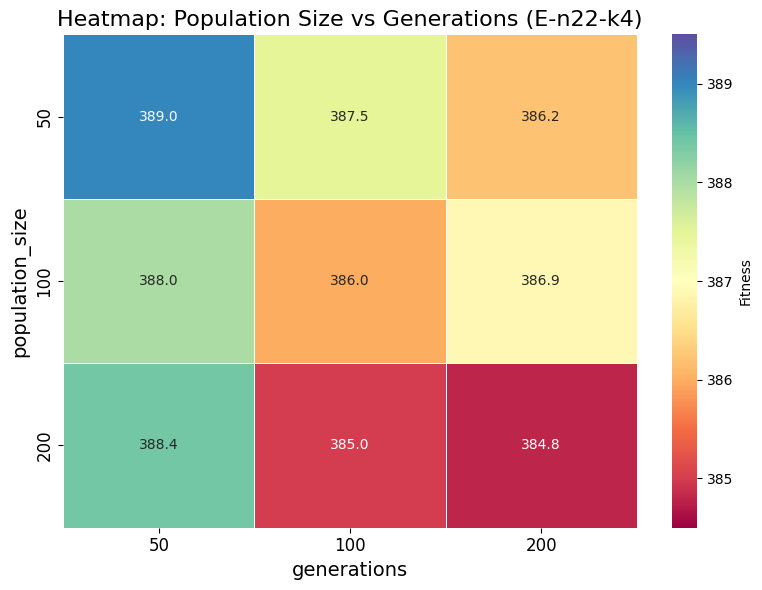
\includegraphics[width=0.3\textwidth]{image/4/parameter/ga/22_4.png} &
        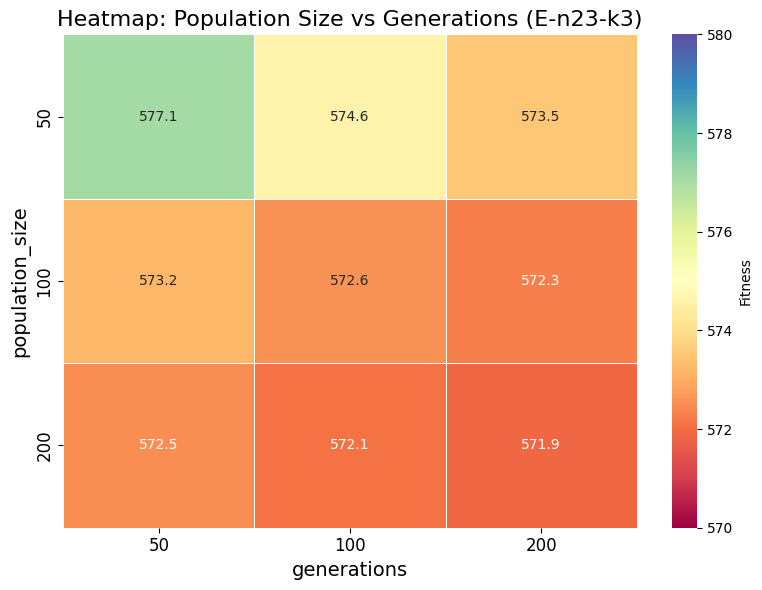
\includegraphics[width=0.3\textwidth]{image/4/parameter/ga/23_3.png} &
        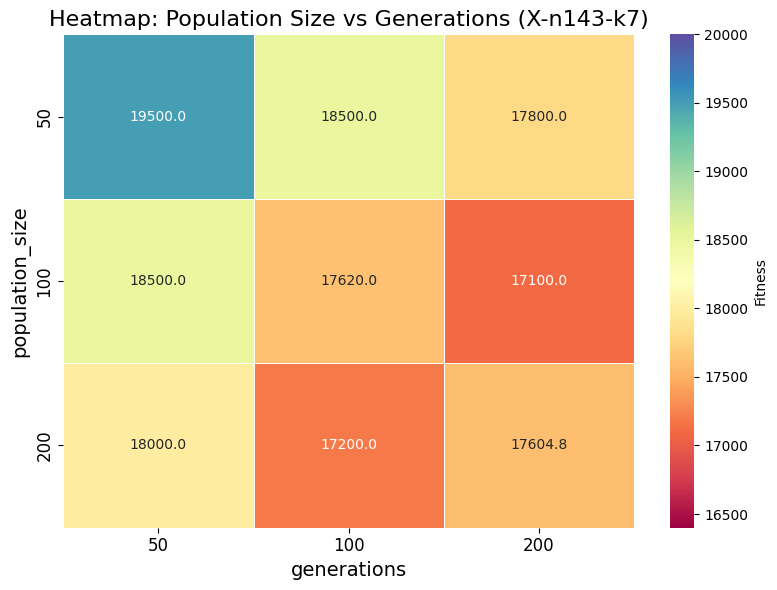
\includegraphics[width=0.3\textwidth]{image/4/parameter/ga/143_7.png} \\
        \small (a) E-n22-k4.evrp & \small (b) E-n23-k3.evrp & \small (c) X-n143-k7.evrp \\
        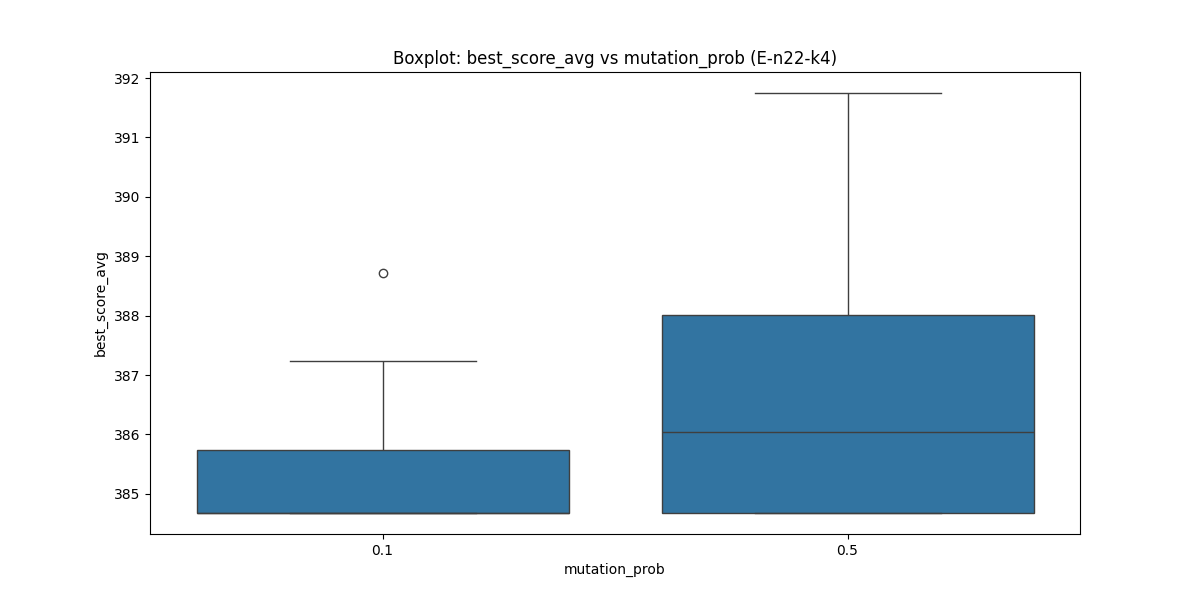
\includegraphics[width=0.4\textwidth]{image/4/parameter/ga/E-n22-k4_boxplot_mutation_prob.png} &
        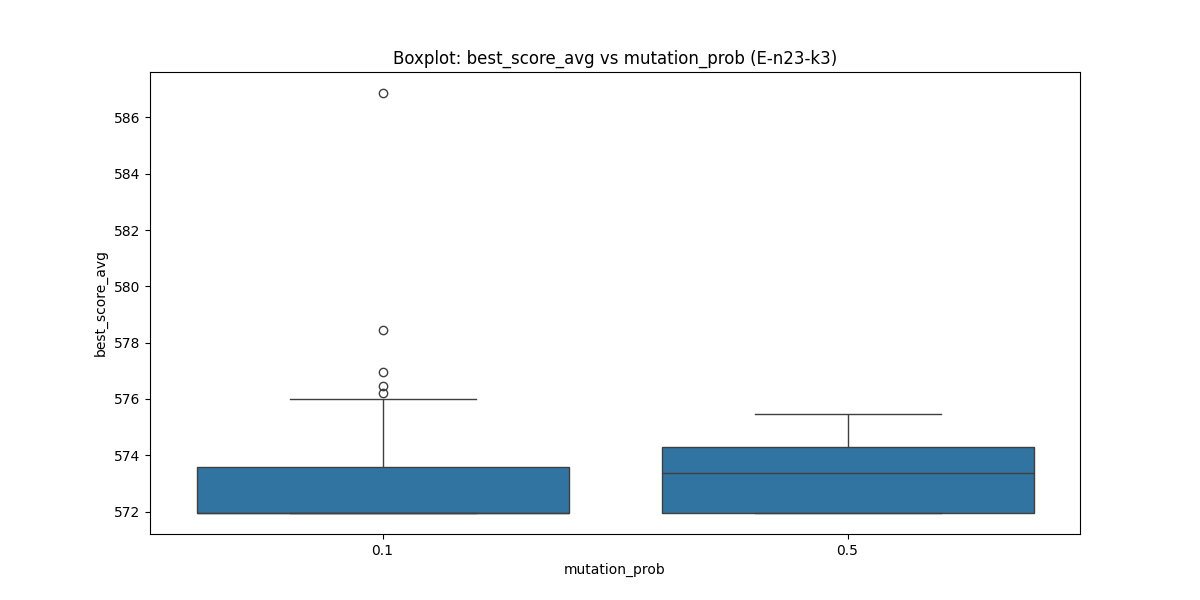
\includegraphics[width=0.4\textwidth]{image/4/parameter/ga/E-n23-k3_boxplot_mutation_prob.png} & \\
        \small (d) E-n22-k4.evrp & \small (e) E-n23-k3.evrp & \\
    \end{tabular}
    \caption{(Top) Heatmaps of performance under different GA settings; (Bottom) Boxplots of mutation probability effects for GA on selected EVRP instances.}
    \label{fig:ga-parameter-analysis}
\end{figure}
\paragraph{Parameter Analysis for GA.}
Figure~\ref{fig:ga-parameter-analysis} provides an in-depth visualization of how key Genetic Algorithm (GA) parameters affect the performance on the EVRP benchmark.

Firstly, the heatmaps (a–c) demonstrate that increasing the population size and the number of generations consistently leads to improved solution quality, as indicated by lower fitness values.  
A larger population size enhances the diversity of the genetic pool, promoting broader exploration of the search space and reducing the risk of premature convergence.  
Simultaneously, a greater number of generations provides the algorithm with more opportunities to refine solutions through selection, crossover, and mutation processes.  
However, the benefits of increasing these parameters exhibit diminishing returns beyond certain thresholds, particularly when moving from moderate to very large values.  
This suggests that while promoting diversity and iterative refinement is critical, excessively large settings may introduce significant computational overhead without commensurate gains in solution quality.

Secondly, the boxplots (d–e) examine the effects of different mutation probabilities.  
For the \textit{E-n22-k4} instance, a lower mutation rate (0.1) yields more concentrated and stable fitness distributions, suggesting that limited yet controlled random perturbations are sufficient to guide the search effectively in smaller-scale problems.  
Conversely, for the \textit{E-n23-k3} instance, a mutation probability of 0.5 slightly improves performance, implying that greater exploration is advantageous in more complex search landscapes to escape local optima.  
These observations indicate that the optimal mutation intensity is instance-dependent: lower mutation rates promote convergence stability, whereas higher rates enhance exploration in rugged solution spaces.

Overall, these findings highlight the complementary roles of each GA parameter:

\begin{itemize}
    \item \textbf{Population Size}: Governs genetic diversity and global exploration capacity; larger sizes enhance exploration but with diminishing returns beyond a certain point.
    \item \textbf{Number of Generations}: Determines evolutionary depth; more generations enable deeper refinement of solutions.
    \item \textbf{Mutation Probability}: Balances exploration and exploitation; lower rates stabilize convergence, while higher rates encourage escaping local optima.
\end{itemize}

Careful tuning of these parameters ensures that the Genetic Algorithm maintains a robust balance between exploration and exploitation, ultimately achieving high-quality and stable solutions across diverse EVRP instances.

\begin{figure}[!h]
    \centering
    \begin{tabular}{ccc}
        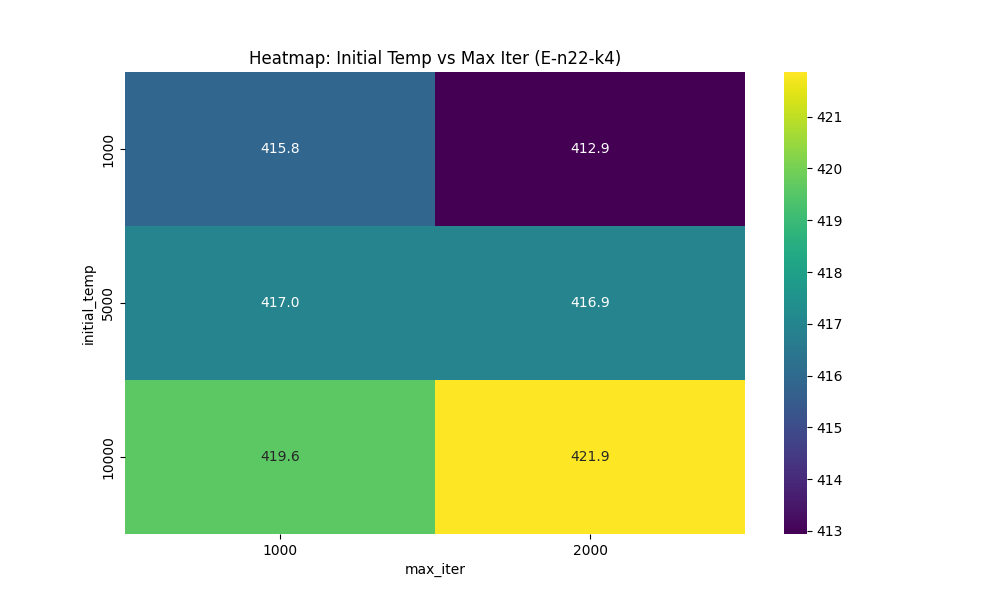
\includegraphics[width=0.3\textwidth]{image/4/parameter/sa/E-n22-k4_heatmap_temp_iter.png} &
        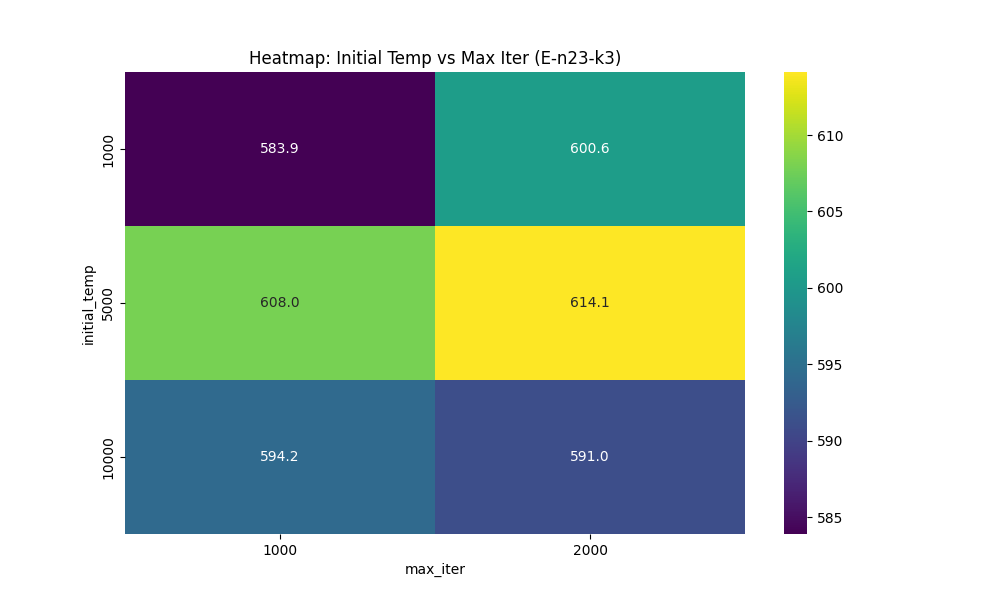
\includegraphics[width=0.3\textwidth]{image/4/parameter/sa/E-n23-k3_heatmap_temp_iter.png} &
        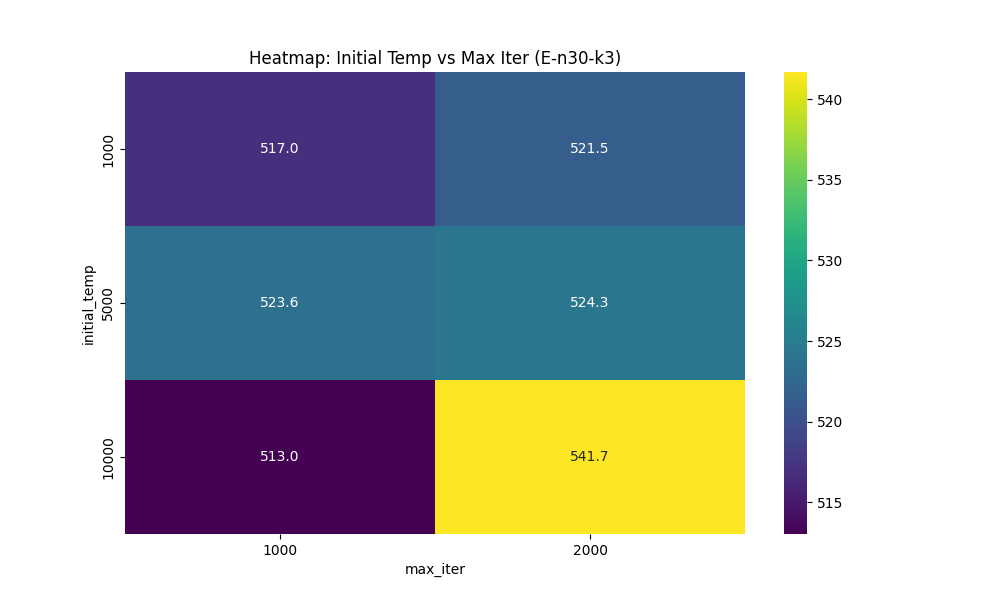
\includegraphics[width=0.3\textwidth]{image/4/parameter/sa/E-n30-k3_heatmap_temp_iter.png} \\
        \small (a) E-n22-k4.evrp & \small (b) E-n23-k3.evrp & \small (c) E-n30-k3.evrp \\
        
        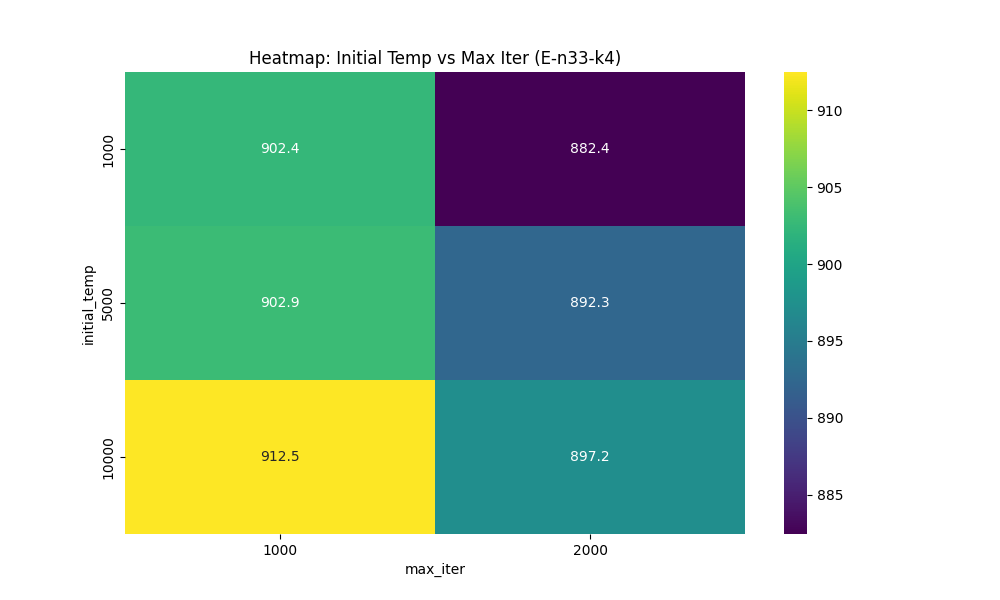
\includegraphics[width=0.3\textwidth]{image/4/parameter/sa/E-n33-k4_heatmap_temp_iter.png} &
        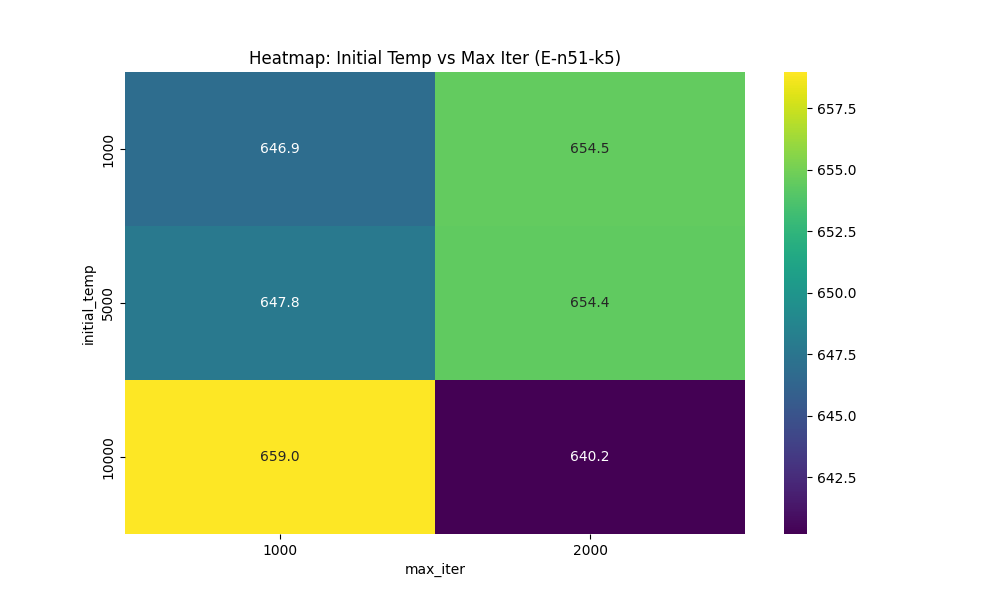
\includegraphics[width=0.3\textwidth]{image/4/parameter/sa/E-n51-k5_heatmap_temp_iter.png} &
        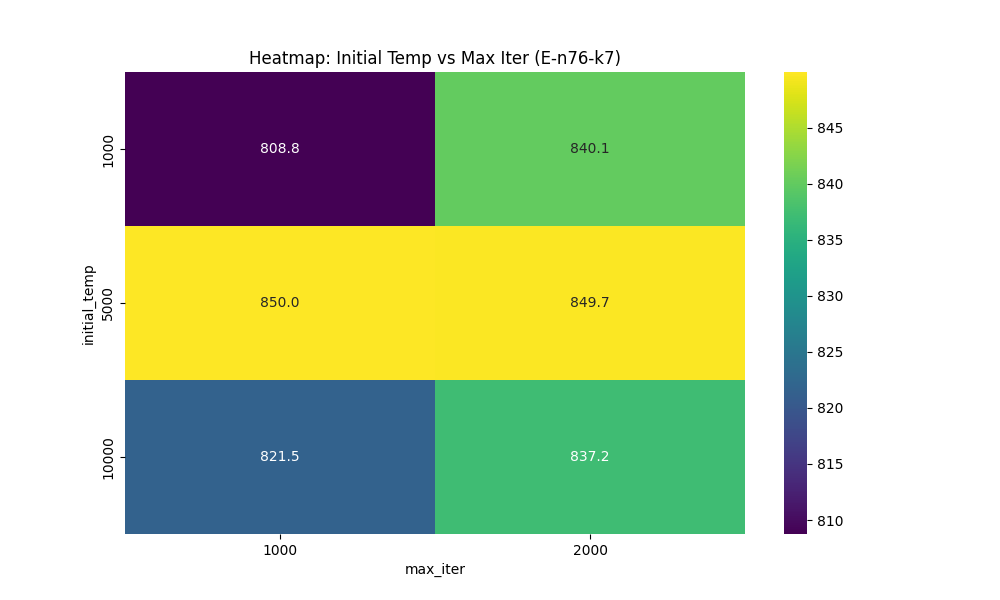
\includegraphics[width=0.3\textwidth]{image/4/parameter/sa/E-n76-k7_heatmap_temp_iter.png} \\
        \small (d) E-n33-k4.evrp & \small (e) E-n51-k5.evrp & \small (f) E-n76-k7.evrp \\
        
        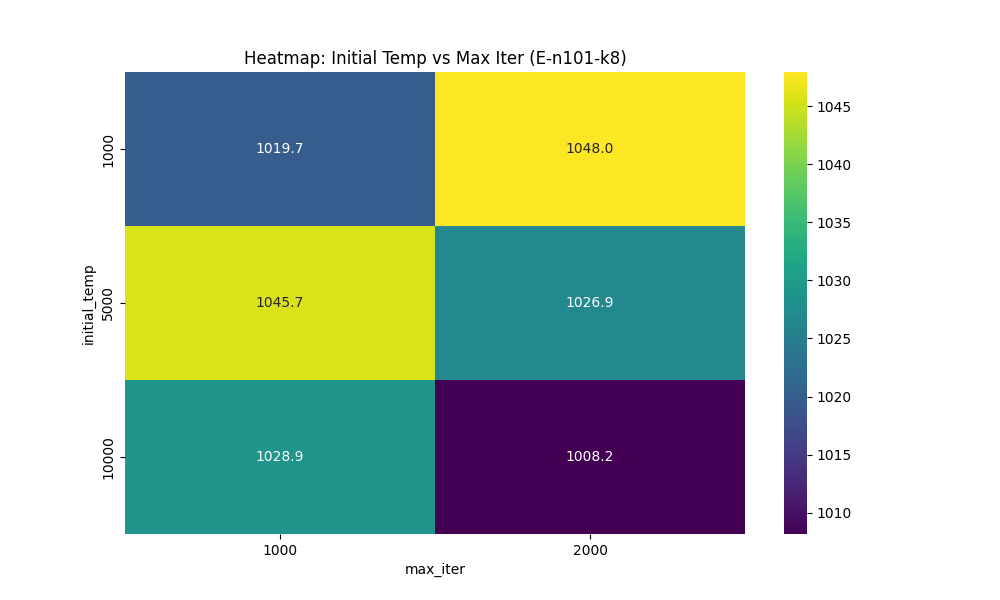
\includegraphics[width=0.3\textwidth]{image/4/parameter/sa/E-n101-k8_heatmap_temp_iter.png} &
        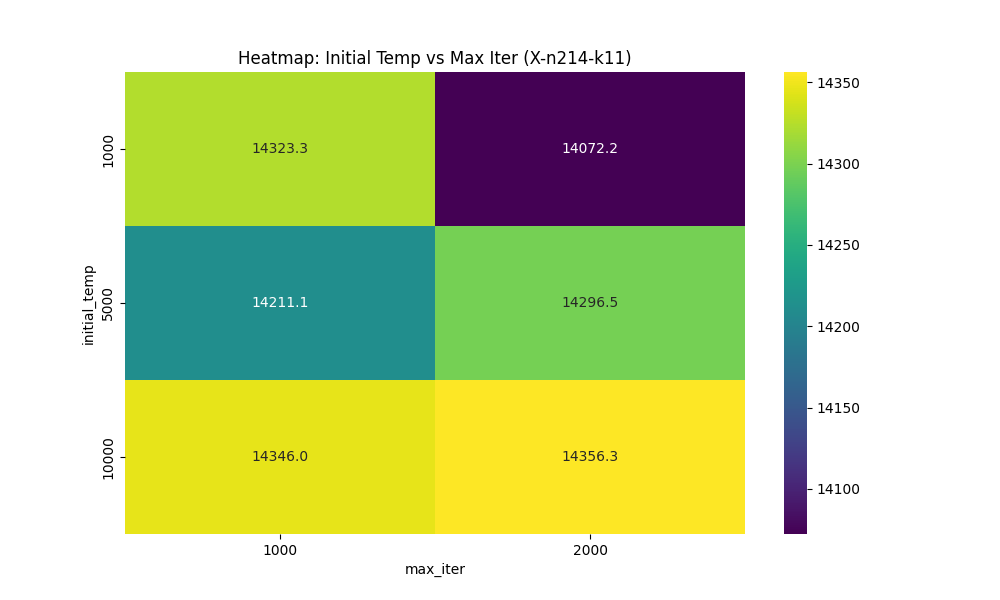
\includegraphics[width=0.3\textwidth]{image/4/parameter/sa/X-n214-k11_heatmap_temp_iter.png} &
        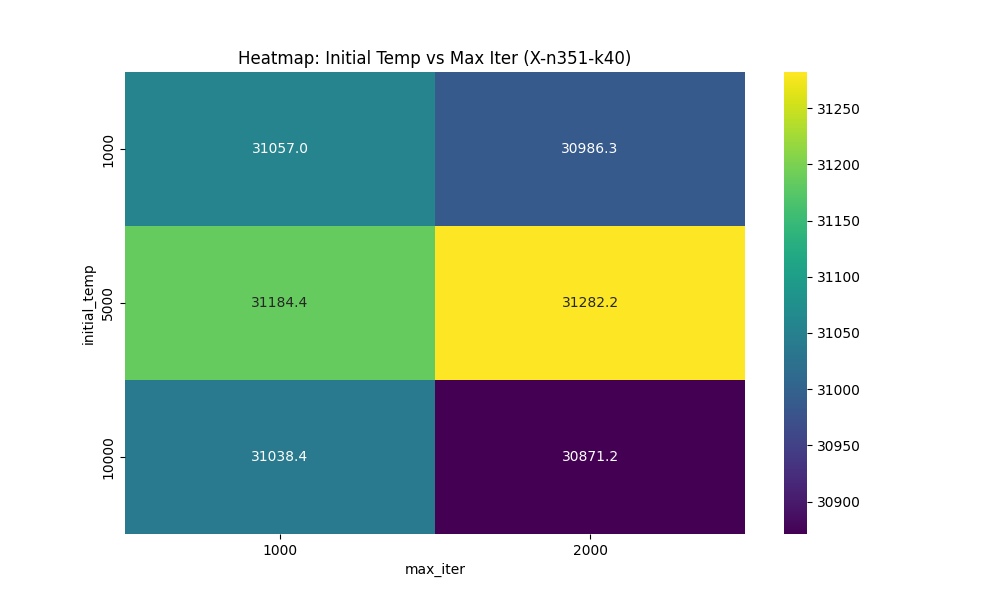
\includegraphics[width=0.3\textwidth]{image/4/parameter/sa/X-n351-k40_heatmap_temp_iter.png} \\
        \small (g) E-n101-k8.evrp & \small (h) X-n214-k11.evrp & \small (i) X-n351-k40.evrp \\
    \end{tabular}
    \caption{Parameter sensitivity analysis on Simulated Annealing (SA) over different EVRP instances.}
    \label{fig:sa-parameter-heatmaps}
\end{figure}
\noindent
\paragraph{Parameter Sensitivity Analysis for SA.}
Figure~\ref{fig:sa-parameter-heatmaps} illustrates the impact of \textbf{initial temperature} and \textbf{maximum iterations} on the performance of Simulated Annealing (SA) across various EVRP instances.

Overall, increasing the \textbf{maximum number of iterations} consistently improves solution quality by enabling more thorough exploration of the search space, particularly for smaller instances such as \textit{E-n22-k4} and \textit{E-n33-k4}.  
However, for moderately complex instances like \textit{E-n30-k3} and large-scale instances such as \textit{X-n351-k40}, the marginal gains from additional iterations diminish, suggesting the existence of a computational efficiency-saturation point.

The role of \textbf{initial temperature} appears to be more instance-dependent.  
For smaller problems, setting a \textbf{lower initial temperature} facilitates faster convergence by limiting unnecessary random exploration in early search phases, leading to quicker stabilization and lower final fitness values.  
In contrast, for larger-scale instances such as \textit{X-n214-k11}, the influence of the initial temperature is less significant, indicating that extensive search iterations are more crucial than initial exploration intensity.


\begin{figure}[!h]
    \centering
    \begin{tabular}{cccc}
        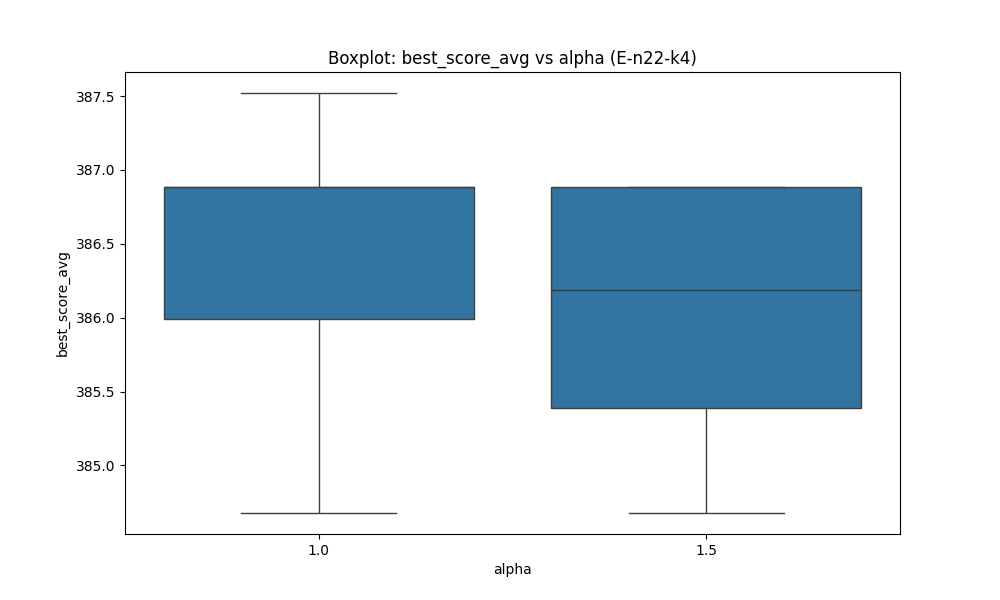
\includegraphics[width=0.22\textwidth]{image/4/parameter/aco/E-n22-k4_boxplot_alpha.png} &
        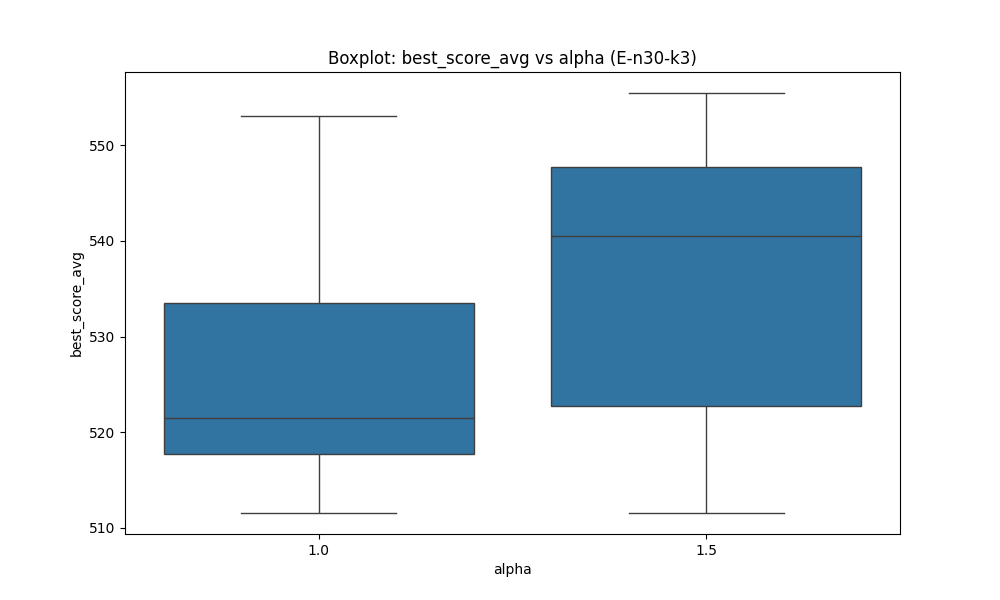
\includegraphics[width=0.22\textwidth]{image/4/parameter/aco/E-n30-k3_boxplot_alpha.png} &
        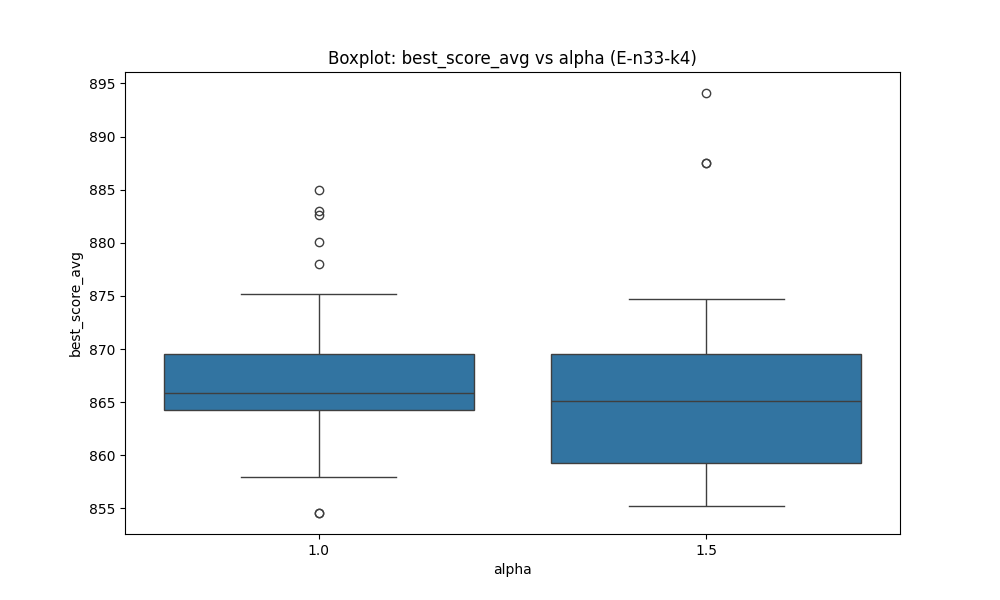
\includegraphics[width=0.22\textwidth]{image/4/parameter/aco/E-n33-k4_boxplot_alpha.png} &
        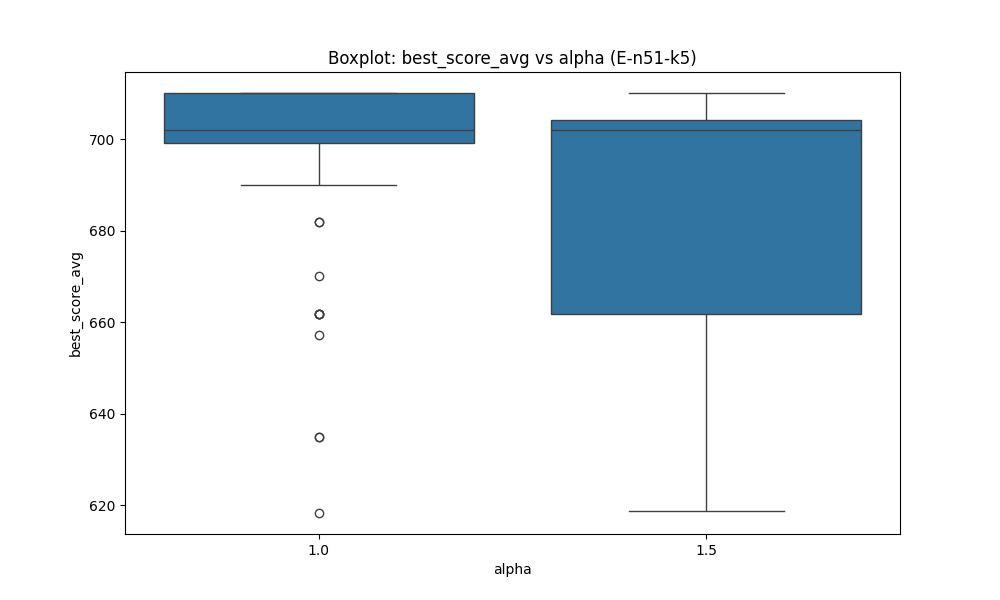
\includegraphics[width=0.22\textwidth]{image/4/parameter/aco/E-n51-k5_boxplot_alpha.png} \\
        \small (a) E-n22-k4.evrp & \small (b) E-n30-k3.evrp & \small (c) E-n33-k4.evrp & \small (d) E-n51-k5.evrp \\
        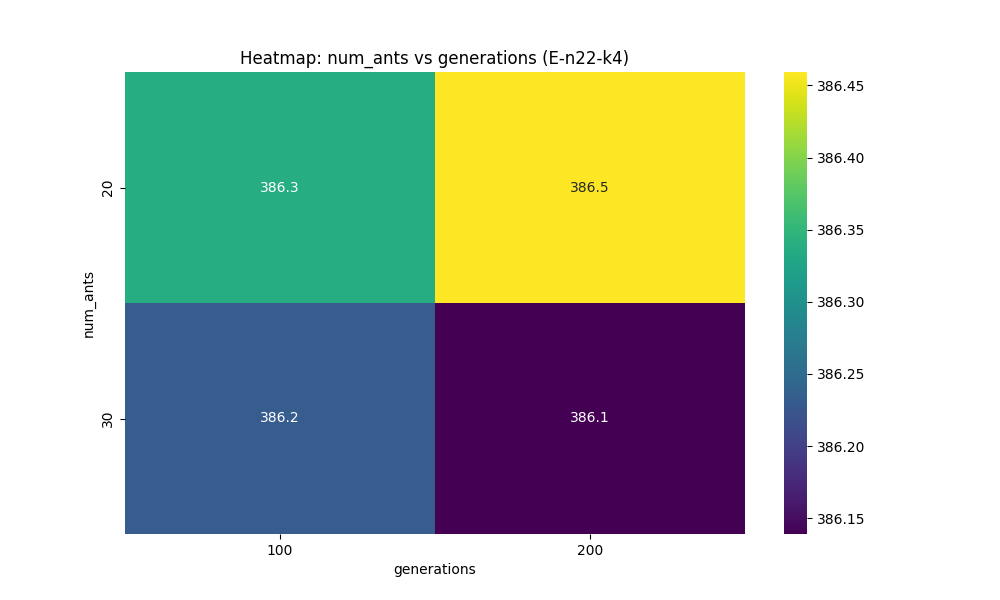
\includegraphics[width=0.22\textwidth]{image/4/parameter/aco/E-n22-k4_heatmap_ants_gen.png} &
        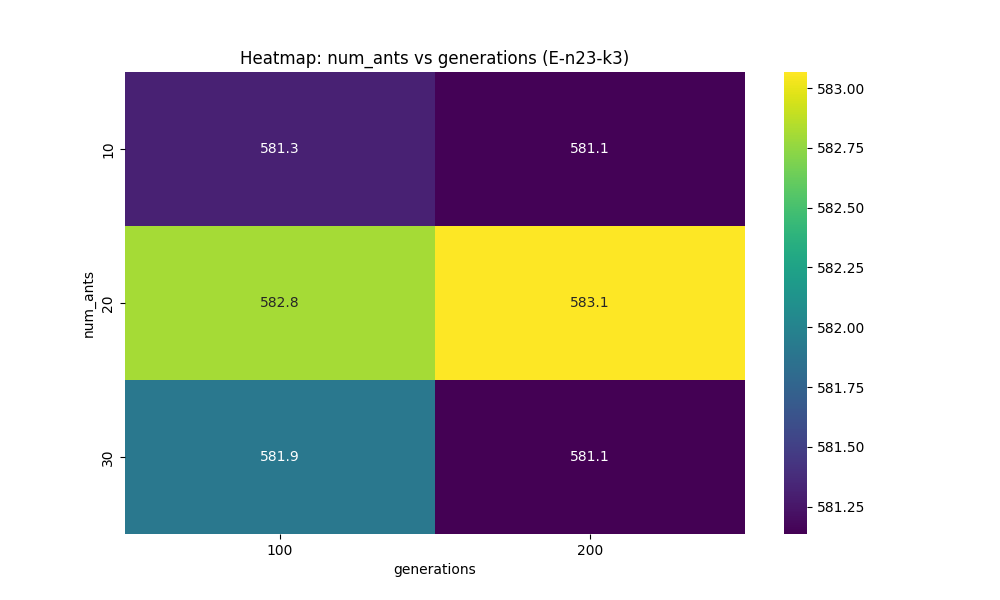
\includegraphics[width=0.22\textwidth]{image/4/parameter/aco/E-n23-k3_heatmap_ants_gen.png} &
        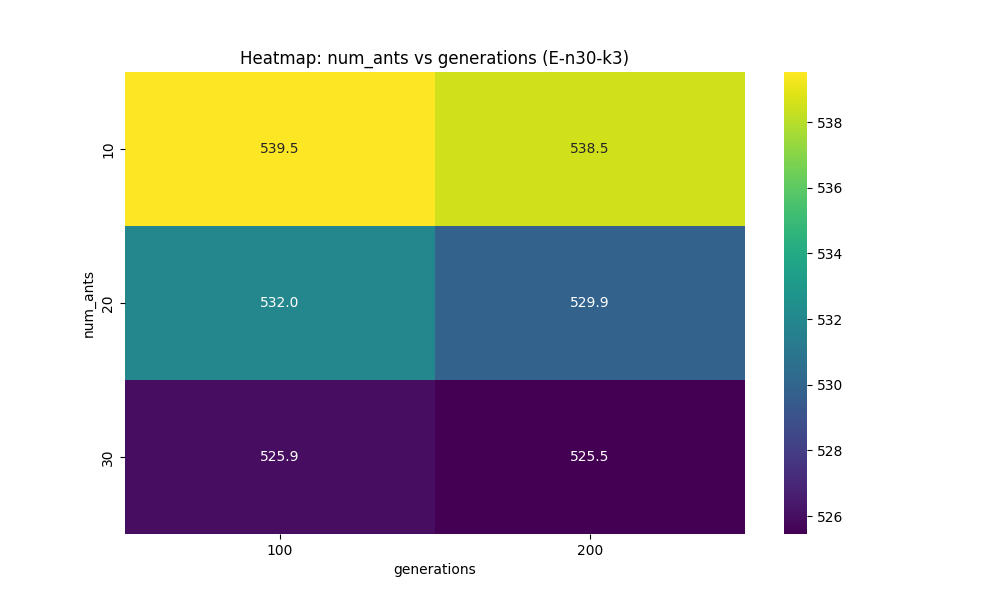
\includegraphics[width=0.22\textwidth]{image/4/parameter/aco/E-n30-k3_heatmap_ants_gen.png} &
        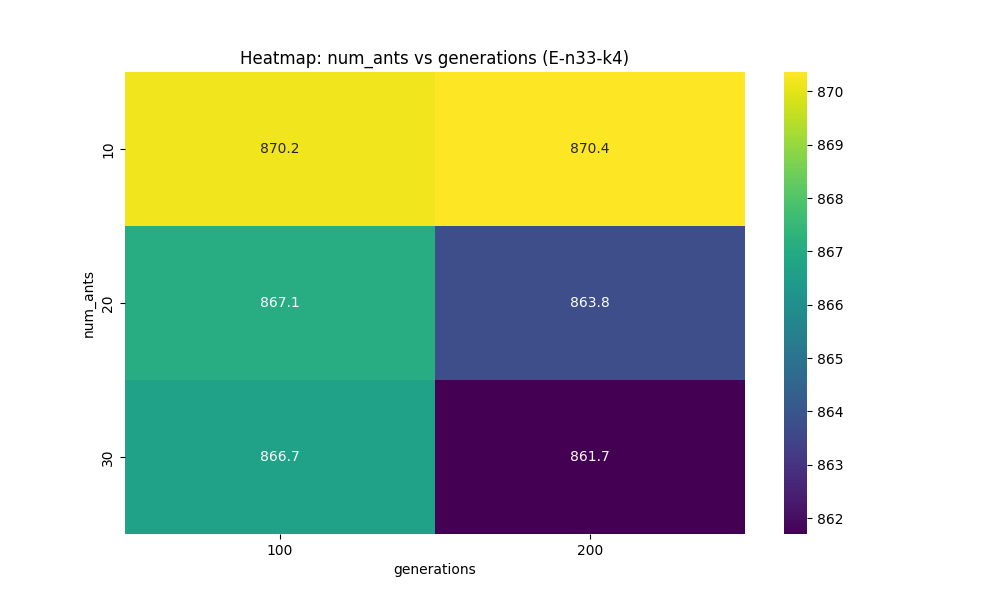
\includegraphics[width=0.22\textwidth]{image/4/parameter/aco/E-n33-k4_heatmap_ants_gen.png} \\
        \small (e) E-n22-k4.evrp & \small (f) E-n23-k3.evrp & \small (g) E-n30-k3.evrp & \small (h) E-n33-k4.evrp \\
    \end{tabular}
    \caption{(Top) Boxplots of different $\alpha$ values in ACO; (Bottom) Heatmaps of ant numbers vs generations for ACO parameter sensitivity analysis on selected EVRP instances.}
    \label{fig:aco-parameter-analysis}
\end{figure}
\noindent
\paragraph{Parameter Sensitivity Analysis for ACO.}
Figure~\ref{fig:aco-parameter-analysis} presents the sensitivity analysis of Ant Colony Optimization (ACO) parameters on selected EVRP instances.

The boxplots (a--d) show the influence of different $\alpha$ values, which control the relative importance of pheromone trails during solution construction. 
On smaller instances such as \textit{E-n22-k4} and \textit{E-n30-k3}, increasing $\alpha$ from 1.0 to 1.5 slightly improves solution quality, indicating that stronger pheromone guidance accelerates convergence.
However, for larger instances like \textit{E-n51-k5}, a higher $\alpha$ introduces greater solution variability, suggesting that excessive pheromone reliance can lead to premature convergence and instability.

The heatmaps (e--h) illustrate the impact of varying the number of ants and generations.
In general, increasing both parameters improves solution quality, particularly on medium-scale instances like \textit{E-n30-k3} and \textit{E-n33-k4}.
Nevertheless, for certain cases such as \textit{E-n23-k3}, increasing the number of ants beyond a threshold does not yield consistent improvements, implying that search redundancy may counteract exploration benefits.
\section{Discussion}
\label{sec:discussion}

The comprehensive experimental results provide several important insights into the effectiveness, robustness, and scalability of the proposed perturbation-driven metaheuristic algorithms for solving the Electric Vehicle Routing Problem (EVRP).

\subsection{Substantial Improvements over Greedy Baseline}
Across all instances, the Greedy Search baseline exhibits significantly higher mean tour lengths and larger standard deviations compared to the proposed algorithms (GA, ACO, SA). 
This confirms that the integration of structured perturbations and local search modules dramatically improves both solution quality and robustness.
The improvement remains consistent across small, medium, and large-scale instances, demonstrating that simple greedy heuristics are insufficient for handling the complex energy and load constraints inherent in EVRP.

\subsection{Effectiveness Hierarchy: GA $>$ ACO $>$ SA}
Among the metaheuristics, GA consistently achieves the best performance, followed by ACO and then SA. 
GA not only yields the lowest best, mean, and maximum fitness values, but also maintains the highest stability (smallest standard deviation) across all instances.
This validates the advantage of GA’s design, which balances global exploration and local refinement through adaptive crossover, mutation, and local search strategies.  
ACO benefits from pheromone-guided search and delivers stable results but is still slightly less effective due to limited adaptability under dynamic constraints.
SA exhibits the largest performance variability, particularly on large-scale instances, reflecting the risk of local minima entrapment in purely temperature-driven exploration.

\subsection{Scalability to Large-Scale Instances}
As the instance size increases (e.g., X-n573-k30, X-n685-k75), all algorithms experience natural degradation in solution quality and stability.
However, the relative ranking remains unchanged: GA continues to outperform ACO and SA, demonstrating superior scalability.
This indicates that the perturbation-driven design principles generalize well even under extreme problem sizes and complexity.

\subsection{Qualitative Analysis Confirms Solution Rationality}
The solution visualizations further validate the quantitative findings.  
GA and SA solutions exhibit well-structured, logical, and compact routing patterns, systematically covering all customers while minimizing redundant paths and excessive charging visits. 
Greedy solutions, in contrast, show chaotic, fragmented tours with frequent depot returns.
ACO solutions are reasonably organized but sometimes suffer from slight over-exploration due to heavy pheromone reliance.

\subsection{Parameter Sensitivity Reveals Key Design Principles}
The parameter sensitivity analysis reveals that:
\begin{itemize}
    \item For \textbf{GA}, larger population sizes and more generations generally enhance performance, while moderate mutation probabilities strike a better balance between exploration and convergence.
    \item For \textbf{SA}, increasing the number of iterations consistently improves solutions, while tuning the initial temperature is important for small to medium problems.
    \item For \textbf{ACO}, carefully balancing pheromone importance ($\alpha$) and controlling the number of ants and generations is crucial; overly strong pheromone influence or excessive ants can destabilize performance.
\end{itemize}
These observations emphasize the necessity of fine-tuning search parameters based on problem scale and characteristics to achieve optimal results.

\paragraph{Impact of Code Design Enhancements.}
The superior performance of all three algorithms is further attributed to the algorithmic enhancements incorporated into the codebase:
\begin{itemize}
    \item The adoption of \textbf{iterated 2-opt} and \textbf{3-opt} local search ensures strong intra-route optimization.
    \item The introduction of \textbf{perturbation mechanisms} (e.g., adaptive mutation in GA, layered pheromone perturbation in ACO, reheating in SA) enhances global exploration while maintaining feasible solutions.
\end{itemize}


\newpage

\chapter{Conclusion}
\newpage
\label{sec:Conclusion}
\section{Summary of Work}

This study addresses the Electric Vehicle Routing Problem (EVRP), a challenging extension of the classical Vehicle Routing Problem (VRP) that incorporates energy constraints alongside traditional load and route constraints.  
To tackle this problem, three advanced metaheuristic frameworks were developed: a Greedy-Search Genetic Algorithm (GA), a Simulated Annealing (SA), and an optimized Ant Colony Optimization (ACO) method.  
Each framework integrates problem-specific perturbation mechanisms, multi-stage local search procedures, and adaptive parameter control strategies to effectively balance global exploration and local refinement.

The proposed algorithms were systematically evaluated on a suite of benchmark instances from the IEEE WCCI-2020 EVRP Competition, encompassing both small- and large-scale scenarios with varying levels of complexity.  
A unified experimental protocol was adopted, measuring metrics such as total travel distance, feasibility rate, solution stability (standard deviation), and computational efficiency across multiple independent runs.  
Furthermore, comprehensive ablation studies were conducted to assess the individual contributions of critical components, including local search operators, perturbation-based diversification, and adaptive operator selection mechanisms.

Experimental results demonstrate that the perturbation-driven metaheuristic frameworks significantly outperform the baseline Greedy Search in both solution quality and robustness.  
Among the three proposed methods, GA consistently achieves the best overall performance across all instances, followed by ACO and SA.  


\section{Achievement}

This research systematically addressed the challenges of the Electric Vehicle Routing Problem through the design, development, and evaluation of perturbation-driven metaheuristic frameworks.  
A systematic literature review was first conducted to critically survey existing metaheuristic methods for EVRP and related vehicle routing variants, highlighting the role of perturbation mechanisms in improving search effectiveness.  
Baseline implementations of Genetic Algorithm, Simulated Annealing, and Ant Colony Optimization tailored for energy-constrained VRPs were developed, ensuring full compliance with load, energy, and feasibility constraints.  
Building upon insights from the literature, structured perturbation strategies were designed and incorporated into SA and ACO, inspired by the success of adaptive perturbation in GA, thereby enhancing both exploration and exploitation capacities.  
Domain-specific repair mechanisms and multi-stage local search enhancements were also integrated into each algorithm, substantially improving solution feasibility, convergence stability, and overall route quality.  
Extensive experiments were conducted on the standardized EVRP benchmark set, systematically comparing the perturbation-enhanced algorithms against baseline methods in terms of total travel distance, robustness across multiple runs, and computational efficiency.  
Finally, the scalability and generalizability of the proposed frameworks were demonstrated through consistent performance improvements across both small- and large-scale EVRP instances.


\section{Limitation}

While the proposed perturbation-driven metaheuristic frameworks demonstrate strong performance on the EVRP benchmark datasets, several limitations are acknowledged.

First, the algorithms were primarily evaluated on static benchmark instances with deterministic travel distances and fixed energy consumption rates.  
In real-world EVRP applications, additional complexities such as dynamic customer demands, variable traffic conditions, and stochastic energy consumption may significantly impact solution quality.

Second, although perturbation and local search strategies effectively improve solution feasibility and quality, they introduce additional computational overhead, especially for large-scale instances.  
The scalability of the current frameworks may be constrained when addressing very large, real-time EVRP scenarios without further acceleration mechanisms.

Third, parameter settings for each algorithm were tuned through manual grid search based on benchmark performance.  
Automated or adaptive hyperparameter optimization strategies were not explored, which could potentially enhance algorithmic robustness across different problem domains.

Finally, the current study focuses on single-objective optimization, minimizing only the total travel distance.  
Realistic EVRP formulations often involve multiple conflicting objectives, such as minimizing energy consumption, customer service time windows, or environmental impact, which remain to be addressed in future work.

\section{Future Work}
\subsection{Enhancing Intelligent and Dynamic Perturbation Mechanisms}

While the current perturbation strategies have proven effective in improving solution quality, future research should focus on developing more intelligent and dynamically adaptive perturbation mechanisms tailored to the evolving characteristics of EVRP solutions.  
Rather than relying on static or manually designed perturbation operators, future approaches should explore adaptive strategies that adjust perturbation intensity, operator selection, and targeted regions based on real-time search feedback~\cite{hulagu2021electric}.

For instance, dynamically identifying "critical zones"—such as densely clustered customer areas or segments with near-battery depletion—and applying targeted perturbations could more efficiently guide the search away from local optima.  
Moreover, integrating learning-based frameworks, such as reinforcement learning for operator selection or self-tuning mechanisms for perturbation strength based on search progress, presents a promising avenue to enhance both exploration and exploitation capabilities~\cite{liu2023electric}.

Designing perturbation mechanisms that are sensitive to solution structure, instance complexity, and current search stagnation will be crucial for enabling scalable, adaptive, and robust EVRP optimization in increasingly realistic and dynamic environments.


\subsection{Enhancing Problem Modeling Realism}

An important avenue for future research is to advance the realism of EVRP problem formulations.  
While most existing studies focus on minimizing total travel distance, practical logistics operations often prioritize minimizing overall operational costs, encompassing factors such as energy consumption, driver salaries, and vehicle maintenance or depreciation.  
Furthermore, with growing pressure to achieve sustainable transportation goals, future EVRP models should integrate environmental objectives, such as minimizing total energy consumption or carbon emissions, thus aligning optimization efforts with green logistics strategies.

Energy consumption modeling also warrants further sophistication.  
Instead of assuming a constant consumption rate per unit distance, future work should incorporate dynamic factors including traffic congestion, road elevation changes, weather conditions, varying vehicle payloads, regenerative braking, and auxiliary energy usage (e.g., heating and cooling systems).  
Accounting for these real-world influences is essential for building robust and practically deployable EVRP solutions~\cite{fang2025two}.

Additionally, the common assumption of homogeneous fleets limits the applicability of many current models.  
Future research should extend EVRP formulations to heterogeneous or mixed fleets, accommodating both electric and internal combustion vehicles with diverse capacities, driving ranges, and regulatory restrictions, such as limited access in low-emission zones.  
Finally, a more realistic depiction of charging operations is needed: instead of assuming uniform recharging behavior, future models should capture nonlinear charging dynamics, where charging rates vary based on the battery’s state of charge and external grid conditions~\cite{zhang2023robust}.



\subsection{Incorporating Operational Constraints and Charging Technologies}

Another important avenue for future research is to enrich the operational realism of EVRP models. Current approaches often oversimplify the charging process, typically assuming uniform charging rates and ignoring real-world infrastructure limitations~\cite{rahman2016review}.  
Future studies should model the coexistence of multiple charging technologies—including Level I (slow charging), Level II (standard charging), and Level III (fast charging)—and account for their availability not only at public facilities but also at customer sites. Key factors such as varying investment costs, installation feasibility, and heterogeneous charging speeds should be incorporated to better reflect practical deployment scenarios~\cite{margaritis2016electric,awasthi2017optimal}.

Moreover, modeling dynamic charging environments is crucial, where charging speeds, costs, and grid availability fluctuate over time. Capturing phenomena such as peak versus off-peak electricity pricing, daily variations in charging performance, and the influence of smart grid load management would significantly improve the realism of EVRP models.

Beyond achieving feasibility, future EVRP frameworks should explicitly aim to \textbf{minimize the number of charging stops}. Reducing charging frequency not only enhances route efficiency but also shortens operational delays and lowers energy expenditures. Achieving this requires a tighter integration between routing decisions and charging planning.

Additionally, future models should incorporate realistic operational constraints, such as legal limits on driving hours, mandatory driver rest periods, and flexible customer service windows~\cite{xu2017joint}.  
Investigating the alignment of driver breaks with charging opportunities could further enhance schedule efficiency and practicality.  

Finally, jointly optimizing both vehicle routing and charging station placement remains an open and promising research challenge that could yield substantial operational benefits.




\newpage

\pagenumbering{roman}

\printbibliography[heading=bibintoc]

\end{document}
